% doc type
\documentclass[12pt]{article}

% set up supplemental section
\newcommand{\beginsupplement}{%
	\setcounter{table}{0}
	\renewcommand{\thetable}{S\arabic{table}}%
	\setcounter{figure}{0}
	\renewcommand{\thefigure}{S\arabic{figure}}%
}

% format page, paragraph
\usepackage[margin=1in]{geometry}
\usepackage{lineno}
\linenumbers
\usepackage{setspace}
\doublespacing
\usepackage[utf8]{inputenc}
\usepackage[hidelinks]{hyperref}
\usepackage{authblk}

% bib - uses better biblatex
\usepackage[style=apa,backend=biber]{biblatex}
\addbibresource{./Zotero_adr_dwi.bib}

% figures and tables
\usepackage{graphicx}
\graphicspath{ {./} }
\usepackage{multirow}
\usepackage[table,xcdraw]{xcolor}
\usepackage{url}
\usepackage{float}
\usepackage{longtable}
\usepackage{rotating}
\usepackage{float}
\usepackage{subfig}
\usepackage{caption}
\DeclareCaptionLabelFormat{adja-page}{\hrulefill\\#1 #2 \emph{(previous page)}}

% code
\usepackage{listings,lstautogobble}
\lstset{language=R,
	basicstyle=\small\ttfamily,
	otherkeywords={0,1,2,3,4,5,6,7,8,9},
	morekeywords={TRUE,FALSE},
	deletekeywords={data,frame,length,as,character},
	autogobble=true
}
\renewcommand\lstlistingname{R Code}

% math
\usepackage{amsmath}
\usepackage{caption}
\DeclareCaptionType{equ}[R Code][]

% title page info
\title{Longitudinal Study of Concussion-Related Diffusion MRI Changes in College Athletes: Modeling Tracts via Hierarchical Generalized Additive Models}
\date{}

\author[1,2,*]{Nathan M. Muncy}
\author[1,2]{Heather C. Bouchard}
\author[1,2]{Doug H. Schultz}
\author[1,2]{Maital Neta}
\author[1,2]{Aron K. Barbey}

\affil[1]{Center for Brain, Behavior and Biology, University of Nebraska-Lincoln}
\affil[2]{Department of Psychology, University of Nebraska-Lincoln}
\affil[*]{Corresponding author.	Email: nmuncy2@unl.edu}

% start document
\begin{document}

% title page
\maketitle
\pagebreak


% abstract page
\begin{abstract}
Sports-related traumatic brain injuries affect approximately 3.8 million individuals in the US each year, each triggering a complex sequence of axonal changes. Although diffusion-weighted imaging can quantify these changes, these longitudinal data are difficult to model statistically given issues of dimensionality, interdependence, and non-linear interactions. \textbf{Proposal}: Hierarchical generalized additive models (HGAMs) are well-suited to fit such data with the requisite flexibility and sensitivity to investigate (a) the spatial and temporal concussion-related changes of white matter tracts, and (b) how such changes relate to diagnostic assessments. \textbf{Methods}: We used MRI and ImPACT data collected from 69 college athletes at three visits: start-of-season, post-concussion, and return-to-play. A whole-brain, longitudinal HGAM modeled fractional anisotropy (FA) tract profiles to test for concussion injury- and recovery-related changes, and the source of FA change (whether radial (RD) or axial diffusivity (AD)) was then investigated for identified tracts. We next tested whether such FA changes related to ImPACT metrics and recovery time. \textbf{Results}: For tracts which showed evidence of concussion-related changes, we found that (i) the superior frontal callosal and right cingulum tracts recovered from injury, (ii) the superior parietal callosal, left corticospinal, right anterior thalamic, and right inferior fronto-occipital tracts did not recover, and (iii) the motor callosal, orbital callosal, left arcuate, and right uncinate tracts worsened by return-to-play. Next, we found that RD but not AD was the source of FA change. Finally, we show that tract FA changes relate to the total symptom, visual memory, and visual motor ImPACT metrics as well as recovery time. \textbf{Merit}: HGAMs offer a powerful framework to capture the complex progression of brain injury. Our findings suggest that HGAMs enhance our understanding of the spatiotemporal dynamics of brain injury and may enable more accurate tracking of injury and recovery.

\end{abstract}

\vfill
KEYWORDS: DWI, MRI, GAM, TBI, Concussion\\
\pagebreak


\section{Introduction}
\label{sec:intro}

% Epidemilogic description of TBI in US, athletes
Each year an estimated 1.6 to 3.8 million sports-related concussions occur in the United States \parencite{langlois2006EpidemiologyImpactTraumatic,daneshvar2011EpidemiologySportRelatedConcussion,barkhoudarian2016MolecularPathophysiologyConcussive}. In collegiate sport, concussions during competition occur at a rate of 30.09 per 10,000 athletic events in men's American football and 14.23 per 10,000 athletic events in women's soccer \parencite{pierpoint2021EpidemiologySportRelatedConcussion}. While many concussions (e.g. mild traumatic brain injury (mTBI); see \textcite{mayer2017SpectrumMildTraumatic} and \textcite{silverberg2023AmericanCongressRehabilitation}) may still go under-reported, the incidence of sport-related concussions has risen in recent years \parencite{coronado2015TrendsSportsRecreationRelated,pierpoint2021EpidemiologySportRelatedConcussion}, likely due to increased awareness, evolving diagnostic criteria, improved symptom recognition, and shifts in athletic participation \parencite{yang2017NewRecurrentConcussions}. Despite this growing attention, the understanding of the brain's physiological response through traditional clinical concussion assessments remains limited. Diagnosis of concussions typically involve a multifaceted process to collect different types of information including patient history, neurological examination, symptom inventories, and cognitive testing \parencite{patricios2023ConsensusStatementConcussion}. However, these methods often fall short in detecting the subtle and complex pathophysiological changes that occur post-injury.

% % mTBI sequelae description
% % TODO: Include info to link to framework section (evolve over time, recover)
% % TODO: reinforce language about demyelination
% Sport-related injury of the head can result from the rapid application of shear, tensile, and/or compressive strains that are consequential for sensitive neural structures, particularly neuronal axons that are especially vulnerable given their cytoskeletal structure \parencite{elsayed2008BiomechanicsTraumaticBrain,johnson2013AxonalPathologyTraumatic,bar-kochba2016StrainRatedependentNeuronal}. Collectively, the various biochemical cascades associated with axonal injury are referred to as diffuse or traumatic axonal injury \parencite{krieg2023IdentifyingPhenotypesDiffuse}, although `diffuse' is a misnomer as axonal injury is commonly found in parasagittal fibers e.g. splenium of corpus callosum \parencite{jang2020DiagnosticProblemsDiffuse,fork2005NeuropsychologicalSequelaeDiffuse,meythaler2001CurrentConceptsDiffuse,johnson2013AxonalPathologyTraumatic,lindsey2023DiffusionWeightedImagingMild}. Initially, disruption may be evident as axons are stretched or sheared beyond their compensatory mechanisms \parencite[e.g. spectrin elongation;][]{dubey2020AxonalActinspectrinLattice}, resulting in primary injuries of axolemmal mechanoporation, disconnection, and disruption as well as breakage of actin-spectrin complexes, microtubules, and neurofilaments. Secondary injury mechanisms are then triggered by changes to the cytoskeletal and axolemmal properties. Microtubule disruption results in the accumulation of axonal transport products, and increased intracellular calcium activates proteolytic calpains which results in neurofilament compaction and spectrin degradation \parencite{shin2020AxonalTransportDysfunction,ma2013RoleCalpainsInjuryinduced}. Further, primary and secondary changes to ionic channels and exchangers can result in increased intracellular osmolarity, causing water to move from the extracellular to intracellular space, resulting in swelling and even cytotoxic edema \parencite{baracaldo-santamaria2022RevisitingExcitotoxicityTraumatic}. Separately, dissociation of the myelin sheathes may occur at nodal regions due to proteolysis of their binding proteins and sites \parencite{krieg2023IdentifyingPhenotypesDiffuse,song2022ConcussionLeadsWidespread}. While such primary and secondary sequelae are sufficient to trigger caspase-mediated axotomy and even apoptosis, this is not necessarily the case and neurons have the machinery to repair themselves \parencite{franze2013MechanicsNeuronalDevelopment,sakai2019InflammationNeuralRepair}. The in vivo investigation of such sequelae in human patients, however, is not directly accessible but of note is that these various injury mechanisms result in differential diffusion trajectories for water molecules. For instance, cellular edema would result in increased tortuosity as axoplasmic water increases and free extracellular decreases, while axotomy would result in increased extracellular water \parencite{rosenblum2007CytotoxicEdemaMonitoring,liang2007CytotoxicEdemaMechanisms,borja2018DiffusionMRImaging,barkhoudarian2016MolecularPathophysiologyConcussive}.

% DWI and mTBI
Diffusion tensor imaging (DTI) is a technique that is widely used to study white matter fibers. For each voxel, a tensor is composed of eigenvalues describing diffusion in para-orthogonal directions. Within white matter, the diffusion trajectory of water is constrained by the axolemma such that the principal diffusion direction (first eigenvalue) is parallel to the axon ($\lambda_\parallel$); this is referred to as axial diffusivity (AD). To describe diffusion perpendicular to the axon ($\lambda_\perp$), radial diffusivity (RD) is calculated as the average of the secondary and tertiary eigenvalues. Likewise, all eigenvalues are averaged to determine the mean diffusivity (MD) of the voxel, and fractional anisotropy (FA) is calculated from these eigenvalues to describe the non-uniformity of diffusion \parencite{mori1999ThreedimensionalTrackingAxonal,lilja2014VisualizingMeyersLoop,lindsey2023DiffusionWeightedImagingMild}. While orders of magnitude exist between the axonal diameter and voxel size, axonal fiber coherence results in tensors that can be used to algorithmically generate tract profiles which approximate the microstructural organization of white matter \parencite{kiselev2021MicrostructureDiffusionMRI,novikov2019QuantifyingBrainMicrostructure,danielian2010ReliabilityFiberTracking,reid2022TractspecificStatisticsBased,sarwar2019MappingConnectomesDiffusion,tournier2007RobustDeterminationFibre}. When mTBI disrupts axonal structure or axolemmal permeability, the resulting atypical diffusion can be measured with DTI and will be reflected in the respective tensors and corresponding tract profiles \parencite{macdonald2007DetectionTraumaticAxonal,macdonald2007DiffusionTensorImaging}. For instance, cellular edema changes the relative ratio of free extracellular water to tortuous axoplasmic water, thereby decreasing RD ($\lambda_\perp$), while demyelination has the reverse effect (increasing RD, driven by the higher ratio of extra- to intra-cellular water). Axotomy, conversely, reduces both AD ($\lambda_\parallel$) and FA as unconstrained water diffuses equally in all directions \parencite{rosenblum2007CytotoxicEdemaMonitoring,liang2007CytotoxicEdemaMechanisms,borja2018DiffusionMRImaging,barkhoudarian2016MolecularPathophysiologyConcussive,pettus1996CharacterizationDistinctSet}.

% Modeling DWI, issues resolved by GAMs
Analysis of Fiber-Tract Quantification \parencite[PyAFQ;][]{yeatman2012TractProfilesWhite,kruper2021EvaluatingReliabilityHuman,kruper2024TractometryHumanConnectome} is a software package that generates white matter tract profiles from preprocessed DWI data. PyAFQ is of particular relevance for concussion research given its approach of subdividing white matter bundles into a number of equidistant nodes and then calculating scalar values for the local, within-tract environment. That is, as concussion-related axonal injury is typically found within a subregion of a given tract \parencite[e.g. parasagittal splenium;][]{jang2020DiagnosticProblemsDiffuse,johnson2013AxonalPathologyTraumatic,lindsey2023DiffusionWeightedImagingMild}, PyAFQ is capable of providing scalar values (e.g. FA) for the injured region that reflect concussion-related changes in diffusion. Such a within-tract node approach is in contrast to other popular methods of diffusion analyses \parencite{lindsey2023DiffusionWeightedImagingMild} which may not be sufficiently sensitive to detect within-tract scalar changes \parencite[e.g. whole-tract or skeletal analyses;][]{smith2006TractbasedSpatialStatistics,fischl2012FreeSurfer} or may not reflect the injury locale (region-of-interest mask). However, while the within-tract resolution afforded by PyAFQ is highly desirable for studying in vivo concussion-related axonal sequelae, a number of statistical considerations become relevant with PyAFQ-derived tractometric profiles: the shape of the profile (non-linear node-scalar interaction), interdependence of node scalars, non-Gaussian scalar distributions, and multiple comparisons with their corresponding corrections \parencite{muncy2022GeneralAdditiveModels,richie-halford2021MultidimensionalAnalysisDetection}.

Generalized additive models \parencite[GAMs;][]{wood2017GeneralizedAdditiveModels,pedersen2019HierarchicalGeneralizedAdditive,stasinopoulos2008GeneralizedAdditiveModels} are an extension of general linear models capable of modeling high-dimensional data which contain non-linear relationships. Where regression models fit data with a linear function, GAMs construct a smooth curve to fit data from a set of basis functions (i.e. splines; also see \textcite{verbyla1999AnalysisDesignedExperiments}). These smooths can capture complex X-Y relationships that would be underfit by models with linear assumptions. Further, non-linear three-way relationships can be modeled via surfaces termed a `tensor product interaction smooth', and hypersurfaces can model even higher dimensional interactions \parencite{baayen2020IntroductionGeneralizedAdditive}. Such capabilities have made GAMs useful in fields such as ecology, paleontology, and linguistics \parencite[e.g.][]{simpson2018ModellingPalaeoecologicalTime,pedersen2019HierarchicalGeneralizedAdditive,schmidt2011SpatiallyExplicitHeight,wieling2011QuantitativeSocialDialectology,simpson2018ModellingPalaeoecologicalTime,wieling2018AnalyzingDynamicPhonetic,murase2009ApplicationGeneralizedAdditive,vanrij2019AnalyzingTimeCourse}, which often model complex non-linear data in high dimensions and/or across multiple factors, and researchers using MRI techniques are beginning to adopt the statistical approach \parencite[e.g.][]{lee2025AtypicalMaturationFunctional,xu2025AgeBSASexspecific,wierenga2018UnravelingAgePuberty,mundo2022GeneralizedAdditiveModels,roy2025DevelopmentArcuateFasciculus,sorensen2021MetaanalysisGeneralizedAdditive,caffarra2024DevelopmentAlphaRhythm}. We previously demonstrated that GAMs are well-fit to model DTI tractometric profiles and provided details to guide decision points in model specification to aid their implementation \parencite{muncy2022GeneralAdditiveModels}. In that work, we used GAMs to investigate cross-sectional group tractometric differences, showcasing the sensitivity and utility of GAMs to detect subtle within-tract group differences in a principled fashion that accounted for the large number of tract nodes, the distribution of scalar values, and avoided the need for `point-wise' comparisons.

% Purpose - (a) extend GAMs for longitudinal DWI, (b) tensor product interaction smooths for multi-modal analyses
Here, we extend the use of GAMs to study concussion injury and recovery in a unique longitudinal dataset that consists of data from collegiate athletes at three visits: baseline (before an athlete sustained a concussion), post-concussion (within approximately 48 hours after diagnosed concussion), and return-to-play (after an athlete was medically cleared to return to full contact). First, we employed hierarchical GAMs to conduct a whole-brain, longitudinal analysis of concussion injury- and recovery-related diffusion (FA) changes. As disruption may occur across multiple tracts, pooling within-subject variance across tracts and visits is critical to better understand injury and recovery; modeling tracts individually would lose such variance, potentially inflating the Type-II error. Then, tracts which differed from baseline were further interrogated in post-hoc analyses to determine whether the change in FA was driven by AD ($\lambda_\parallel$) or RD ($\lambda_\perp$). Second, we used tensor product interaction smooths to build multimodal models with which we tested whether changes in FA related to clinical assessment metrics and recovery time. Such models helped elucidate the connection between physical injury and associated clinical assessments.

Our analyses were guided by mechanistic models of axonal injury and empirical findings from prior concussion research, which together suggest that white matter disruption is (a) spatially localized, (b) evolves nonlinearly over time, and (c) may recovery partially. We hypothesized that: (i) Concussion would lead to decreased FA in the posterior corpus callosum, which would show partial recovery by the return-to-play visit; (ii) FA decreases would be driven primarily by increased RD, rather than AD, consistent with demyelination rather than axotomy; and (iii) FA changes in affected regions would correlate with clinical outcomes, including cognitive performance and symptom burden, particularly during the acute phase (Figure \ref{fig:intro-hyp}) as well as recovery time. By combining high-resolution tractography with longitudinal modeling and theory-informed predictions, this study aims to characterize the spatial and temporal trajectory of white matter injury and its clinical relevance following sport-related concussion.

\begin{figure}[H]
	\centering
	\fbox{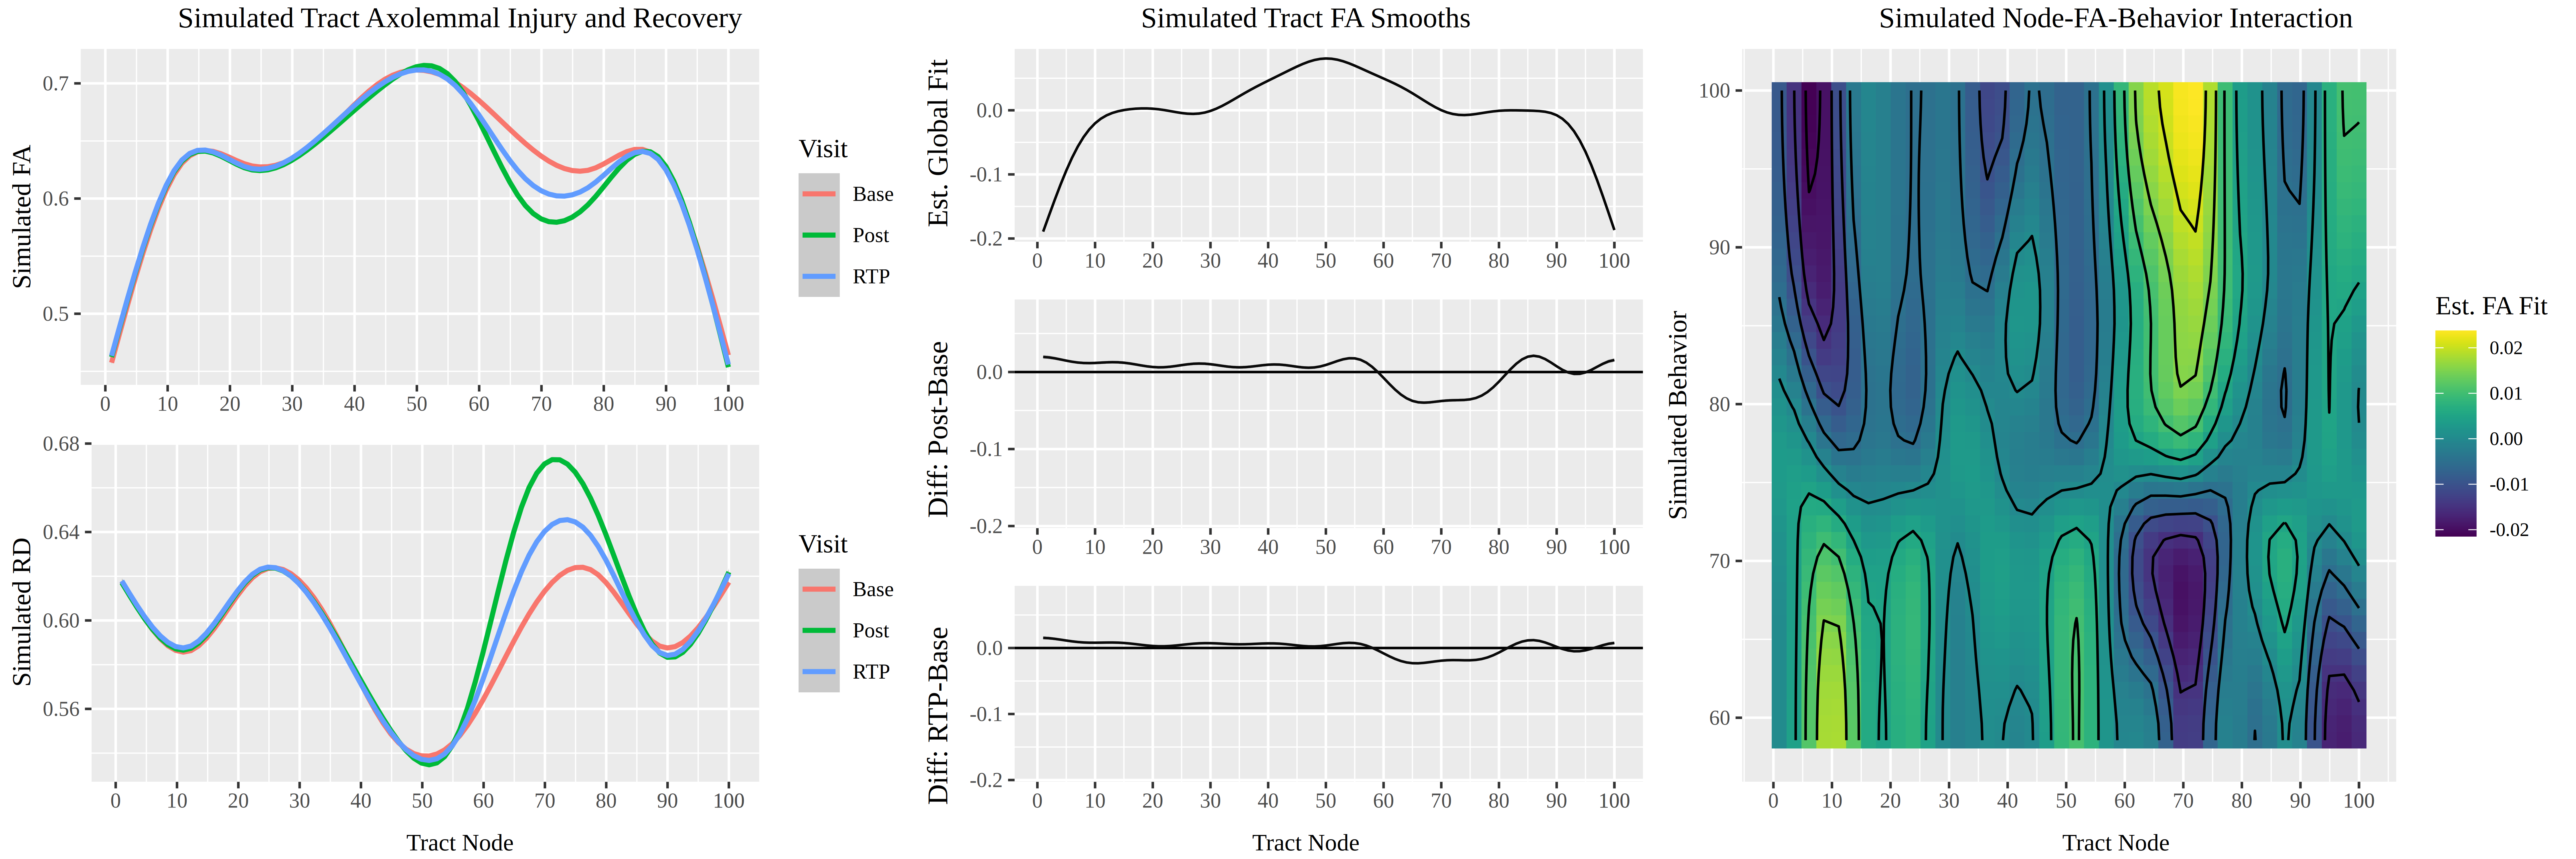
\includegraphics[width=0.95\textwidth]{fig_hypotheses.png}}
	\caption{Simulated data to relate hypotheses to PyAFQ-derived tract profiles and GAM smooths, tensor products. \textbf{Left:} simulated PyAFQ tract profiles of FA (top) and RD (bottom) at three visits: baseline (Red), post-concussion (Green), and return-to-play (Blue). Injury resulted in decreased FA values for nodes 60-80 at Post (top), and FA values are mostly (but not entirely) recovered to Base values by RTP. These FA changes relate to corresponding changes in RD (bottom). \textbf{Middle:} smooths produced by a hierarchical generalized additive model of the tract FA profiles across all visits. The overarching curvature of the tract profile is captured as a main effect in the global fit smooth (top). FA values between nodes 60-80 are lower in Post than Base as evidenced in the difference smooth (middle), and these values are partially recovered at RTP (bottom). \textbf{Right:} a simulated interaction between tract FA values and behavioral response modeled with a tensor product interaction smooth. A linear interaction between behavior and FA values is present in the region of nodes 60-80: higher behavioral values are associated with higher FA values (yellow) while lower behavioral values are related to lower FA values in the same region (blue). Third-order polynomial splines were used to simulate the tract profiles, and behavioral values were shifted by the smallest FA values among the injured nodes. Tract Node = subregion of a segmented white matter tract. FA = fractional anisotropy, RD = radial diffusivity. Base = baseline, Post = post-concussion, RTP = return-to-play.}
	\label{fig:intro-hyp}
\end{figure}


\section{Methods}
\label{sec:meth}

\subsection{Participants}
\label{ssec:meth-part}
Three hundred thirty-six National Collegiate Athletic Association (NCAA) athletes were recruited from men's football and women's soccer programs at the University of Nebraska-Lincoln. Of these participants, 69 (9 female, age = 19.36 $\pm$1.67, range = 17-24) experienced a sport-related concussion during the season and were included in analyses and results reported below. Additional demographic metrics (e.g. race, ethnicity, SES) are omitted to protect participant confidentiality as University athletes are public figures and identification may cause deleterious consequences (but a subset has been reported by \cite{bouchard2024ConcussionRelatedDisruptionsHub}). Due to the limited number of females, and the sport confound that all soccer athletes were female, we combined all participants into a single group. Institutional Review Board approval was obtained at the outset of the study, and participants completed informed consent and assent. MRI and clinical assessment (ImPACT) data were acquired during three visits: enrollment at the beginning of the season (baseline, Base), within approximately 48 hours of diagnosed concussion (post-concussion, Post), and prior to return-to-play (RTP). As MRI and ImPACT (below) data were gathered separately, a number of participants did not contribute MRI and/or ImPACT data across one or more of the visits. Total counts are provided in Table \ref{tbl:meth-demo}.

\begin{table}[H]
	\centering
	\scriptsize
	% Please add the following required packages to your document preamble:
% \usepackage{multirow}
% \usepackage[table,xcdraw]{xcolor}
% Beamer presentation requires \usepackage{colortbl} instead of \usepackage[table,xcdraw]{xcolor}

\begin{tabular}{lccc}
Session & \multicolumn{1}{l}{Sex} & \multicolumn{1}{l}{MRI} & \multicolumn{1}{l}{ImPACT} \\ \hline
 & M & 58 & 56 \\
\multirow{-2}{*}{Base} & \cellcolor[HTML]{C0C0C0}F & \cellcolor[HTML]{C0C0C0}9 & \cellcolor[HTML]{C0C0C0}5 \\
\rowcolor[HTML]{EFEFEF}
\cellcolor[HTML]{EFEFEF} & M & 57 & 45 \\
\rowcolor[HTML]{C0C0C0}
\multirow{-2}{*}{\cellcolor[HTML]{EFEFEF}Post} & {\color[HTML]{333333} F} & {\color[HTML]{333333} 8} & {\color[HTML]{333333} 3} \\
 & M & 49 & 30 \\
\multirow{-2}{*}{RTP} & \cellcolor[HTML]{C0C0C0}F & \cellcolor[HTML]{C0C0C0}7 & \cellcolor[HTML]{C0C0C0}3
\end{tabular}

	\caption{Number of athletes that contributed MRI and ImPACT data across all visits. Base = baseline, Post = post-concussion, RTP = return-to-play. M = Male, F = Female.}
	\label{tbl:meth-demo}
\end{table}


\subsection{ImPACT}
\label{ssec:meth-imp}
We assessed self-reported symptoms and cognitive performance using the Immediate Post-Concussion Assessment and Cognitive Testing (ImPACT), one of the most widely used tools for evaluating concussions \parencite{lovell2005ImPACT200540,dessy2017ReviewAssessmentScales}. Self-reported symptoms were measured with the 22-item Post-Concussion Symptom Scale within ImPACT \parencite{lovell2006MeasurementSymptomsFollowing}. Cognitive performance was assessed through five composite scores derived from ImPACT's computerized neurocognitive tests: verbal memory, visual memory, visual-motor processing speed, impulse control, and reaction time \parencite{lovell2005ImPACT200540}. These assessments were conducted in collaboration with clinicians from our Department of Athletic Medicine and were administered to participants at Base, Post, and throughout their recovery, with the participant's final assessment serving as RTP.


\subsection{MRI Protocol}
\label{ssec:meth-mri}
Magnetic Resonance Imaging data were collected on a 3-Tesla Siemens MAGNETOM Skyra scanner at the Center for Brain, Behavior and Biology (University of Nebraska-Lincoln) utilizing a 20-channel coil. For each of three visits (Base, Post, and RTP), participants contributed T1 and diffusion weighted images (T1w, DWI). T1w Multi-Echo Magnetization Prepared - RApid GRadient Echo (MEMP-RAGE) structural scans were acquired with the following parameters: TR = 2530 ms, TE = 1.69, 3.55, 5.41, and 7.27 ms, flip angle = 7$^{\circ}$, voxel size = 1 mm$^3$, FoV = 256 $\times$ 256, slices = 176 interleaved. DWI scans were acquired via TR = 3000 ms, TE = 95 ms, flip angle = 90$^{\circ}$, voxel size = 1.719 $\times$ 1.719 $\times$ 2.4 mm$^3$, 134 slices, multi-band acceleration factor = 3, directions = 128, bandwidth = 1500 Hz/Px, shells = 1 (b-value = 1000 s/mm$^2$), reference volumes = 6 (b-values = 0 s/mm$^2$; b$_0$). A set of field maps for the DWI scans were collected using the same acquisition direction (anterior-posterior; AP) and reversed (posterior-anterior; PA).


\subsection{MRI Data Processing}
\label{ssec:meth-mri-proc}
Preprocessing and modeling of the DWI data were conducted using FSL v6.0 \parencite{jenkinson2012Fsl} and PyAFQ v1.3.6 \parencite{kruper2021EvaluatingReliabilityHuman,yeatman2012TractProfilesWhite}. First, b$_0$ volumes and acquisition parameters were extracted and combined from the AP and PA field maps, and \lstinline{topup} used the resulting AP-PA b$_0$ file to calculate a distortion correction matrix. Next, a brain mask was constructed via \lstinline{bet}, and then preprocessing of the DWI data was conducted with \lstinline{eddy_openmp}, which incorporated the distortion correction matrix, brain mask, and a volume-acquisition parameter mapping index to produce motion- and distortion-corrected diffusion images.

Whole-brain tractography was computed from the preprocessed DWI by PyAFQ. Constrained spherical deconvolution was used to derive the fiber orientation distribution function (fODF) of each voxel, where constrained-positivity regularization = 1, minimum amplitude $\tau$ = 0.1, mean gray matter diffusivity = 0.0008, mean CSF diffusivity = 0.003, 600 fODF iterations, and spherical harmonics order = 8. Resulting fODFs of each voxel were then utilized to probabilistically generate fiber maps, using one seed per voxel for each dimension, a maximum turning angle of 30$^\circ$, step size = 0.5 mm, and a length range = 50-250 mm. The resulting fibers were parcellated into individual tracts via \textit{a priori} inclusion (waypoint) and exclusion regions of interest \parencite{wakana2007ReproducibilityQuantitativeTractography}. These tracts were then compared to a fiber probability map \parencite{hua2008TractProbabilityMaps} and any fibers which traverse low-probability spaces were removed from the tract. Any fibers with a length 3+ standard deviations from the tract average, or 4+ standard deviations from the average path centroid, were removed as well. Lastly, each tract was then resampled into 100 equidistant nodes (according to a Mahalanobis distance metric) from which averaged diffusion scalars (FA, AD, RD, and MD) were calculated. It was determined upon review of the 28 parcellated tract bundles that bilateral posterior arcuate and vertical occipital tracts were not well identified across all subjects and visits, accordingly analyses only included the remaining 24 white matter tracts. Finally, as scalar values approach zero at the start and end of tracts due to fiber fanning, fitting the distribution becomes rather problematic. We removed the first and last 10 nodes and were subsequently able to fit the data well, and we note that this clipping of the ends is in addition to that already performed by the PyAFQ software.


\subsection{Hierarchical Generalized Additive Models Fit Group Tract Scalars}
\label{ssec:meth-gam}
Hierarchical generalized additive models (HGAMs; \cite{pedersen2019HierarchicalGeneralizedAdditive}) allow for model fits at both global and group levels. That is, it is possible to model both the X-Y relationship that is shared across all levels of a factor (global smooth) and differences that factor levels (group smooths) may have from the global smooth. Further, it is not required that each level of smooth (global, group) contain the same `wiggliness' in the X-Y relationships. Separate smooth curves and wiggliness terms at different factor levels of HGAMs is highly relevant in modeling concussion-related changes within white matter tracts, as the global smooth of the tractometric profile (i.e. scalar values across all nodes) can effectively be held constant when modeling potential changes across visit, and independent wiggliness terms may capture scalar changes unique to one visit. Further, tensor product interaction terms can be used to build multimodal models, investigating the relationship of the tractometric profile with independent metrics such as the ImPACT composite scores. Accordingly, such a model would be capable not only of detecting changes within a tract that result from concussion, but also how such changes relate to clinical assessments. Finally, and critically, HGAMs facilitate conducting longitudinal, whole-brain analyses on tractometric profiles as data from all tracts and across all visits can be included in the same model. Such a specification allows for within-subject pooling of variance across both tract and visit. Where modeling individual tracts results in a creeping Type-I error and the corresponding corrections, concussion (and subsequent recovery) may affect multiple tracts within a subject and such shared variance would be lost when investigating tracts individually. By including all tracts and visits, HGAMs have the capability to not only reduce Type-I but also Type-II errors.

Interpreting GAM output involves considering both the significance and magnitude of the effect, as with the larger family of general linear models. GAMs test against an $H_0$ of flatness, or, whether the inclusion of wiggliness (more effective degrees of freedom) allow for a better fit the data. While smooths are penalized in order to resist over-fitting the data, subtle deflection from flatness can result in statistical, but not necessarily practical significance, and to disentangle this the relative magnitude of the partial effect (distance of the smooth from flat) is considered \parencite{baayen2020IntroductionGeneralizedAdditive}. We also note that the smooth's `confidence intervals' are actually Bayesian posterior credible intervals \parencite{pedersen2019HierarchicalGeneralizedAdditive}, and accordingly we can interpret smooths both with respect to zero and other smooths. When reporting results below, first the statistics are provided for the smooths of interest, which yield information about statistical deflections from flatness anywhere in the smooth. Second, plots will visualize the smooth and credible intervals, allowing interrogation of the partial effect with respect to magnitude, and to this end we plot group smooths in the same range as global smooths so the relative contribution of the partial effect to model fit can be captured. All GAMs were specified using the \lstinline{mgcv} package version 1.9-1 \parencite{wood2017GeneralizedAdditiveModels} in R version 4.3.3 \parencite{rcoreteam2023LanguageEnvironmentStatistical}.


\subsubsection{Whole Brain Longitudinal Difference Model}
\label{sssec:meth-gam-ldi}
To investigate within-tract concussion injury- and recovery-related FA changes we specified an HGAM to test for Post and RTP tract FA differences from Base. First, we calculated the Post-Base and RTP-Base changes in FA ($\Delta$FA); although including original FA values would be ideal, propagating ordered factors (Base $<$ Post $<$ RTP) across an interaction with another factor (tract) loses the original ordered structure. Here, ordered factors were necessary to investigate differences from baseline instead of merely the interaction with visit. $\Delta$FA values were modeled as a function of tract node using thin-plate regression splines (R Code \ref{code:gam-ldi}) and a basis dimensionality of 15 was determined sufficient to fit the tract curves (\lstinline{gam.check(fit_LDI)}). Subjects were treated as a random effect, thereby allowing each subject to have their own intercept across all levels of the factors, the $\Delta$FA distribution was well-fit by a Gaussian distribution with an identity link function, fast Residual Error of Maximum Likelihood (fREML) served as the smoothing parameter estimation method, and 12 threads were used in the computation (run time $\approx$ 45 minutes). Input data consisted of the 24 tracts with good segmentation across all subjects. Notably, we did not include a global smooth for this model, as the $\Delta$FA profile would differ for each tract, and we specified that each tract would have its own wiggliness term; essentially this is a longitudinal model of FA differences which references model `I' in \textcite{pedersen2019HierarchicalGeneralizedAdditive}.

\begin{equ}[H]
	\begin{lstlisting}
		fit_LDI <- mgcv::bam(
		  delta_fa ~ s(subj_id, by=tract_scan, bs="re") +
		    s(node_id, by=tract_scan, bs="tp", k=15) +
		    tract_name+visit_comp+tract_scan,
		  data=df,
		  family=gaussian(),
		  method="fREML",
		  nthreads=12
		)
	\end{lstlisting}
	\caption{$\Delta$FA values are modeled as a function of tract node with thin-plate regression smooths for each tract, accounting for the within-subject factors of tract and visit and using separate wiggliness terms for each tract. \lstinline{delta_fa} = RTP-Base and Post-Base FA differences, \lstinline{subj_id} = subject identifier factor, \lstinline{node_id} = node identifier integer, \lstinline{tract_name} = tract identifier factor, \lstinline{visit_comp} = visit comparison factor (RTP-Base, Post-Base), and \lstinline{tract_scan} = interaction of \lstinline{tract_name} and \lstinline{visit_comp}.}
	\label{code:gam-ldi}
\end{equ}


\subsubsection{Tract Longitudinal Scalar Model}
\label{sssec:meth-gam-lgio}
The model specified in R Code \ref{code:gam-ldi} effectively models the entire longitudinal dataset of $\Delta$FA values, allowing for pooling for variance within a subject across tract and visit, not requiring a multiple comparison correction for modeling all tracts. But as the $\Delta$FA calculation required participants to have data at Post and/or RTP in addition to Base (see Table \ref{tbl:meth-demo}), the analysis could not use all available data. As essentially a post-hoc analysis to further interrogate tract differences across visit, and also what change in scalar (e.g. increased RD) drove the difference in FA, individual tracts were modeled with a longitudinal HGAM with terms for global and group smooths (R Code \ref{code:gam-lgio}). Tract FA values were fit by a beta distribution with a logit link function, AD and RD values were fit with a Gaussian distribution and identity link function, and a gamma distribution with a logit link function fit the MD values. Subjects were again treated as a random effect, with separate intercepts for each scan (Base, Post, RTP), group smooths were allowed their own wiggliness parameter, and the colinearity of global and group smooths was controlled by the `m' parameter. Such a model is similar to model `GI' in \textcite{pedersen2019HierarchicalGeneralizedAdditive}. Finally, an ordered visit factor was included to test for difference in Post and RTP scalar values from Base. Such a model is particularly useful as the test statistic, which describes the flatness of the smooth, provides information about changes from Base values rather than deflections from zero. A model which fits group smooths for each visit is provided in Supplemental Materials (Supplemental R code \ref{supp-code:gam-lgi}).

\begin{equ}[H]
	\begin{lstlisting}
		df$scanOF <- factor(df$scan_name, ordered=T)
		fit_LGIO <- mgcv::bam(
		  <scalar> ~ s(subj_id, scan_name, bs="re") +
		    s(node_id, bs="tp", k=15, m=2) +
		    s(node_id, by=scanOF, bs="tp", k=15, m=1),
		  data=df,
		  family=<family>,
		  method="fREML",
		  nthreads=4
		)
	\end{lstlisting}
	\caption{Tract scalars are modeled as a function of tract node with thin-plate regression splines using both global and group (\lstinline{scan_name}) smooths as well as individual group wiggliness. An ordered factor of scan visit was used to compare Post and RTP to Base. \lstinline{<scalar>} = relevant DWI metric (AD, RD, MD, or FA), \lstinline{scan_name} = visit identifier factor (Base, Post, RTP), \lstinline{scanOf} = ordered factor of \lstinline{scan_name}, \lstinline{<family>} = relevant family and link function for scalar distribution.}
	\label{code:gam-lgio}
\end{equ}


\subsubsection{Tract Longitudinal Scalar Interaction Model}
\label{sssec:meth-gam-lgio-intx}
As noted above, GAMs are capable of modeling higher-dimensional, non-linear interactions through tensor product interaction smooths and hypersurfaces, a property which makes them particularly relevant for multimodal research. We used such a model to test whether concussion injury- and recovery-related changes in tract scalars related to changes in ImPACT composite and total symptom scores (R code \ref{code:gam-lgio-intx}), thereby potentially linking damage within a specific region of a tract to changes in assessment metrics. Tract scalars were modeled as a function of both tract node and ImPACT measure, and the node-ImPACT interaction term was specified such that each visit (Base, Post, RTP) would have a different scalar-node-ImpACT interaction surface. We note the decrease in basis dimensionality for the ImPACT measures thin-plate regression splines from the default value, and that fitting the tensor product interaction smooth also benefited from a slightly higher basis dimensions term for the tract node term. Additionally, and as above (Section \ref{sssec:meth-gam-lgio}), an ordered factor for visit was included to test whether the Post and RTP interaction surfaces differed from that of Base; a model with separate interaction surfaces is provided in Supplemental Materials (Supplemental R code \ref{supp-code:gam-lgi-intx}).

\begin{equ}[H]
	\begin{lstlisting}
		df$scanOF <- factor(df$scan_name, ordered=T)
		fit_LGIO_intx <- mgcv::bam(
		  <scalar> ~ s(subj_id, scan_name, bs="re") +
		    s(node_id, bs="tp", k=15, m=2) +
		    s(imp_meas, by=scan_name, bs="tp", k=5) +
		    ti(node_id, imp_meas, bs=c"tp","tp"), k=c(20,5), m=1) +
		    ti(
		      node_id, imp_meas, by=scanOF,
		      bs=c("tp","tp"), k=c(20,5), m=1
		    ),
		  data=df,
		  family=<family>,
		  method="fREML",
		  nthreads=4
		)
	\end{lstlisting}
	\caption{Tract scalars are modeled as a function of separate 1D node and ImPACT smooths as well as a 2D tensor product interaction surface, with ordered factors used to compare Post and RTP surfaces to Base. \lstinline{imp_meas} = ImPACT composite or total symptom measure.}
	\label{code:gam-lgio-intx}
\end{equ}

Finally, another potentially powerful use of tensor product interaction smooths is to model changes in tract scalars as a function of time. Given the within-tract temporal dynamics of axonal injury and recovery, the ability to model non-linear temporal interactions with scalar changes will help quantify the progression of injury. For such an analysis, however, multiple scans would be required of each participant to effectively track signal associated with recovery. As our data were collected only at Post and RTP, we modeled tract FA differences between Post and RTP (RTP-Post $\Delta$FA) as a function of node and number of days between the two visits (via a model similar to Supplemental R code \ref{supp-code:gam-lgi-intx}). Such an analysis has the potential to identify which tract changes are associated with the longest recovery periods, as presumably less-severe injuries are associated with fewer days between Post and RTP. We also note that few participants had recovery periods longer than 14 days, so any detected interactions at longer recovery periods may be driven by relatively few participants (recovery duration = 9$\pm$5.5 days, recovery duration $>$14 days = 6 participants; 1 outlier omitted (93 days) due to poor model fit).

\subsubsection{ImPACT model}
\label{sssec:meth-gam-impact}
The relationship between visit (Base, Post, RTP), ImPACT composite metrics (verbal memory, visual memory, visual motor, impulse control, and reaction time), and ImPACT total symptom scores were modeled with GAMs to test for changes across assessment visit. As with tract scalar profiles, GAMs were employed as (a) non-linear trends are expected in such metrics and (b) they can model the semi-parametric distributions encountered in several of the metrics. Each ImPACT metric was fit as a function of assessment number, using integer values rather than categorical Base, Post, and RTP (Supplemental R Code \ref{supp-code:gam-impact}); such a specification allowed for modeling evolving changes in assessment metrics rather than comparing main effects across factor levels. Verbal and visual memory composites were converted to proportion scores and modeled with a beta distribution and logit link function, visual motor speed and reaction time were best fit with Gaussian distributions and identity link functions (despite the skewness), and a negative binomial distribution with log link function fit the impulse control and total symptoms well.

When specifying models, whether with ImPACT or DWI data, model fits were reviewed and assessed via \lstinline{mgcv:gam.check()}, and the selection of competing models was aided by \lstinline{itsadug::compareML()}. Pipeline and statistical code are available at the project repository: \url{https://github.com/nmuncy/adr_dwi}.


\section{Results}
\label{sec:res}

\subsection{ImPACT Visual Memory, Reaction Time, and Total Symptoms Show Evidence of Injury and Recovery}
\label{ssec:res-imp}
All models of ImPACT metrics (Section \ref{sssec:meth-gam-impact}), except for impulse control, detected a significant interaction between the ImPACT metric and visit. Boxplots of response quartiles organized by visit are provided in Figure \ref{fig:imp-gam}a (also, see Supplemental Table \ref{supp-tbl:imp-desc}), and estimated fit smooths in Figure \ref{fig:imp-gam}b. Visual memory, reaction time, and total symptoms demonstrated patterns consistent with concussion-related deficits at Post and subsequent recovery at RTP (visual memory: $F_{(1.94, 1.99)}$ = 8.59, \textit{p} $<$ .001; reaction time: $F_{(1.91, 1.99)}$ = 6.18, \textit{p} $<$ .01; total symptoms: $F_{(1.98, 1.99)}$ = 28.74, \textit{p} $<$ .0001), and we note that total symptoms at RTP were much lower than at Base (Figure \ref{fig:imp-gam}, bottom right).

Conversely, while verbal memory and visual motor tests indicate significant non-flatness (verbal memory: $F_{(1.82, 1.96)}$ = 4.34, \textit{p} = .028; visual motor: $F_{(1.86, 1.97)}$ = 8.19, \textit{p} $<$ .001), concussion-related changes were not detected between Base and Post and the statistic is driven by increased performance at RTP. This pattern possibly reflects a lack of sensitivity at Base and/or practice effects. Finally, impulse control was unchanged (i.e. flat) as a function of assessment ($F_{(1.0, 1)}$ = .003, \textit{p} = .95).

\begin{figure}[H]
	\captionsetup{oneside,margin={-112mm,0cm},captionskip=-78mm} % Put caption a-b in top left corner
	\subfloat[]{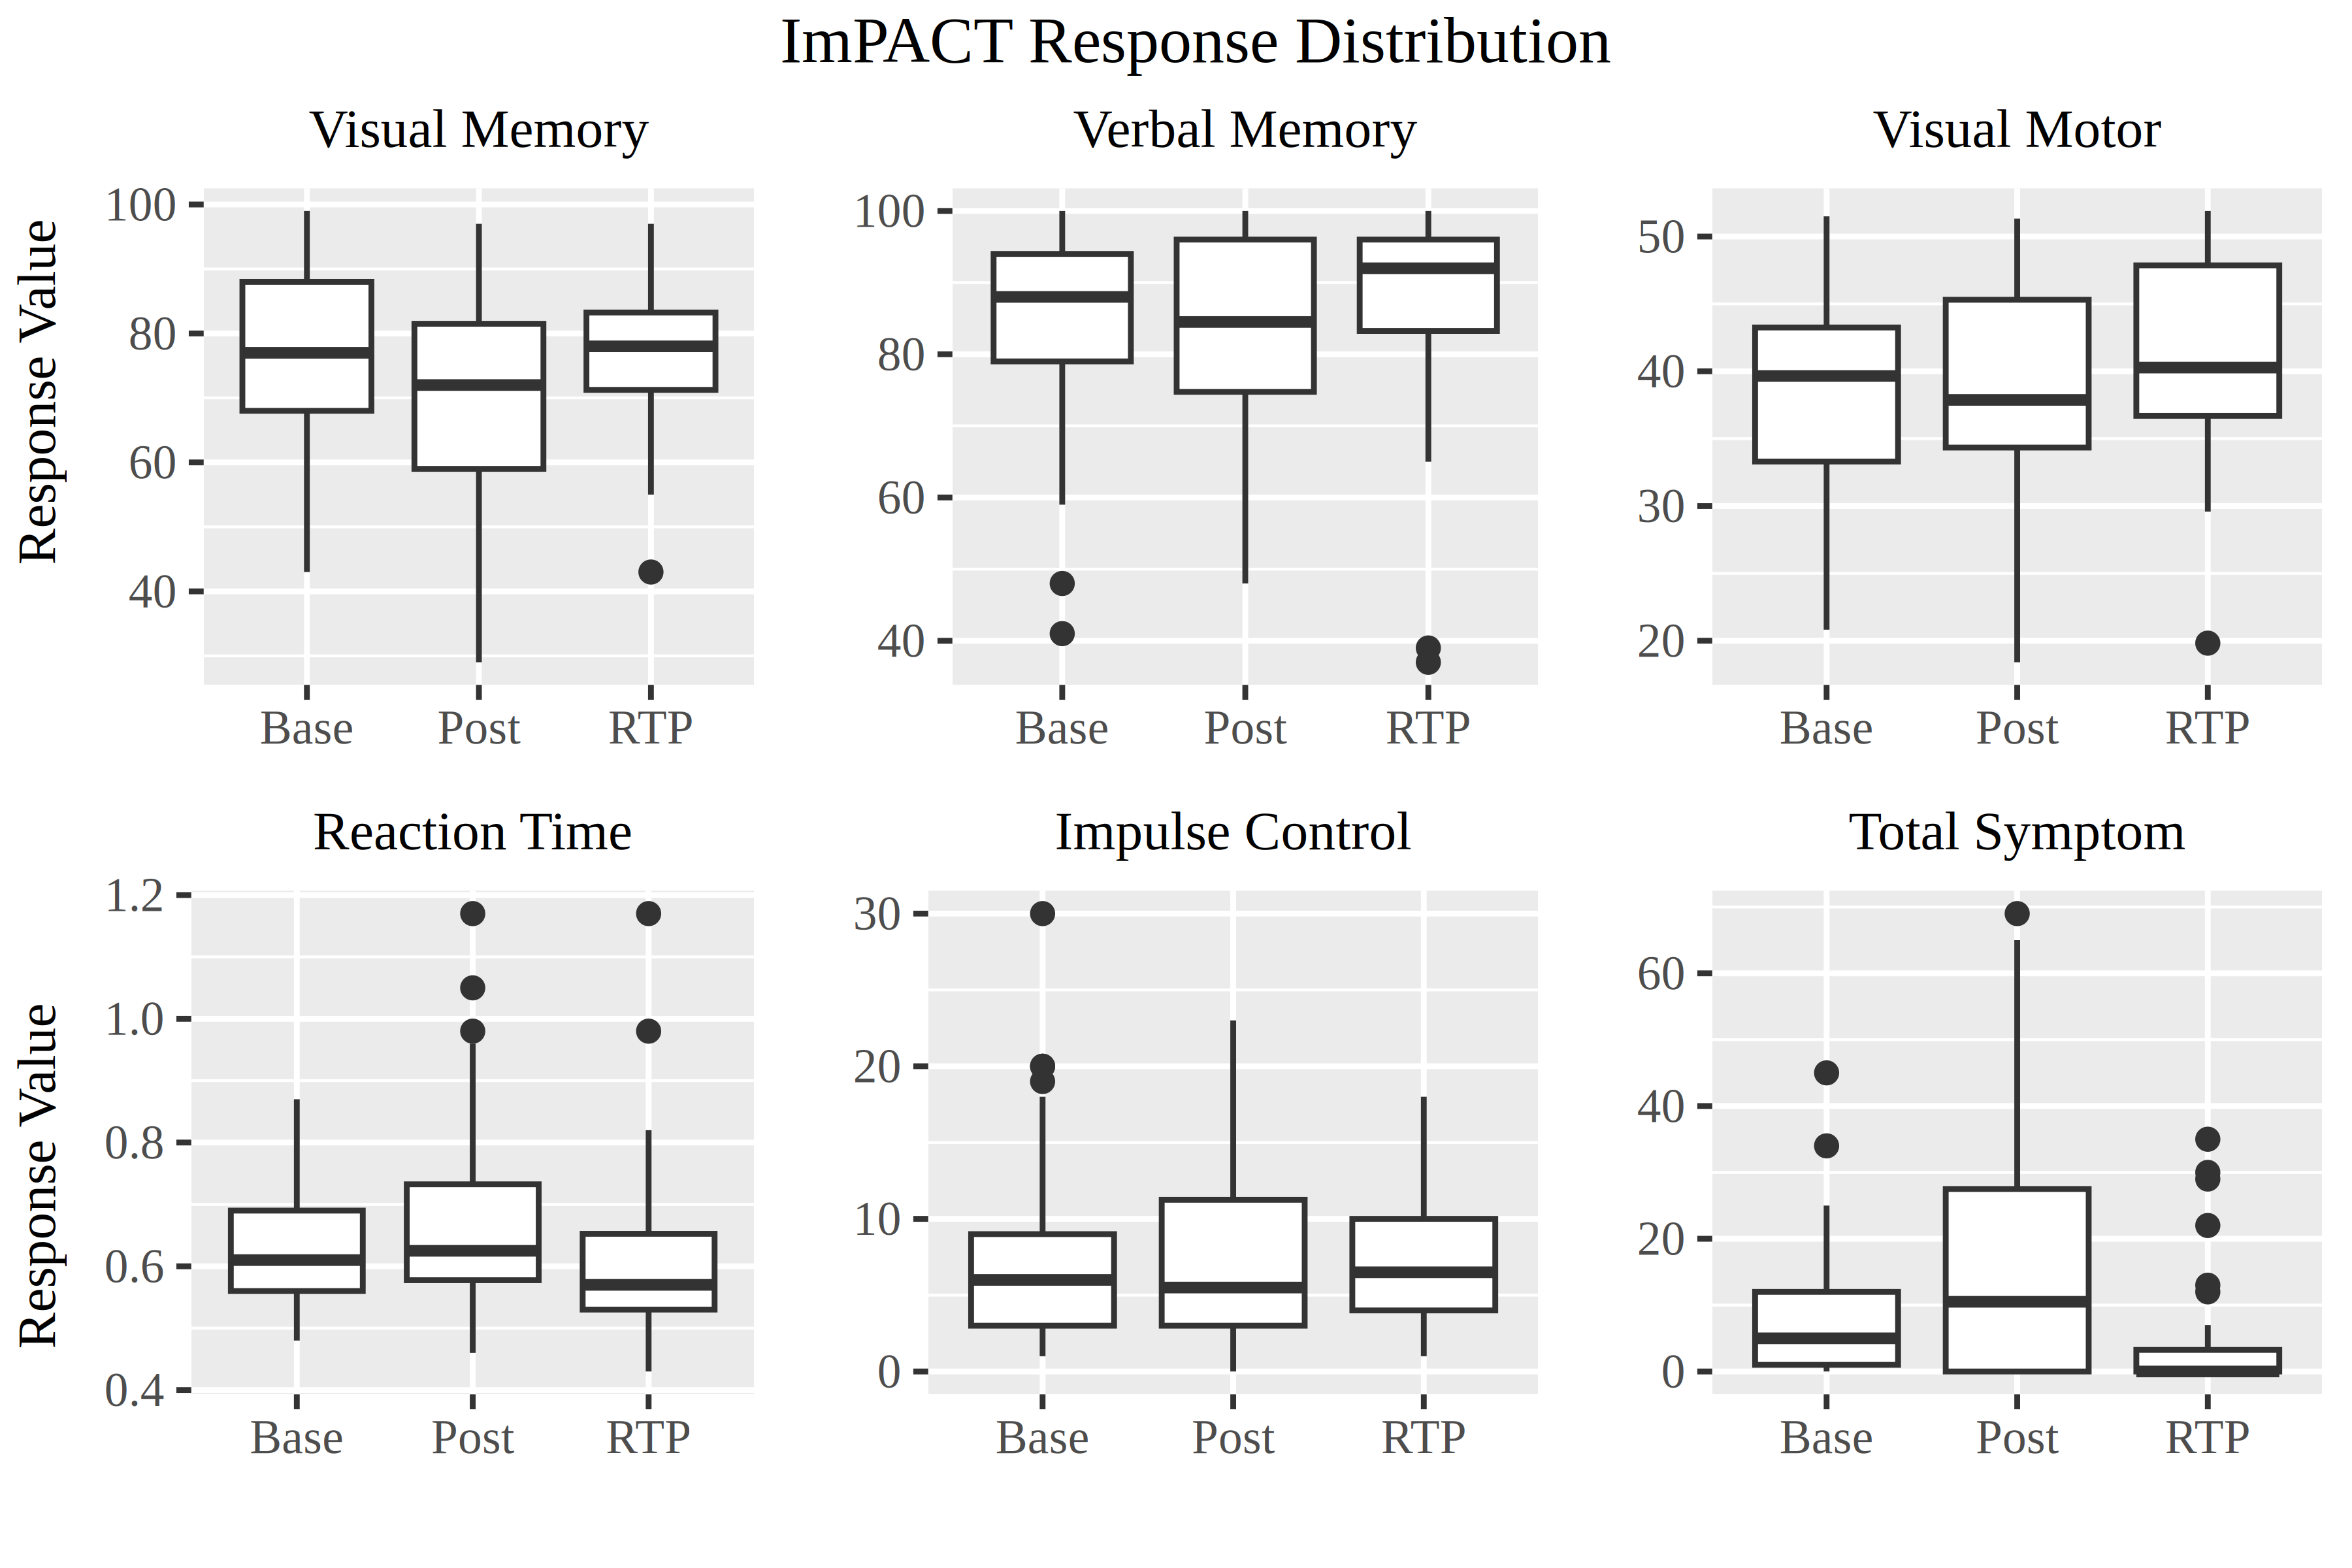
\includegraphics[width=0.7\textwidth]{fit_impact_beh.png}}\\
	\subfloat[]{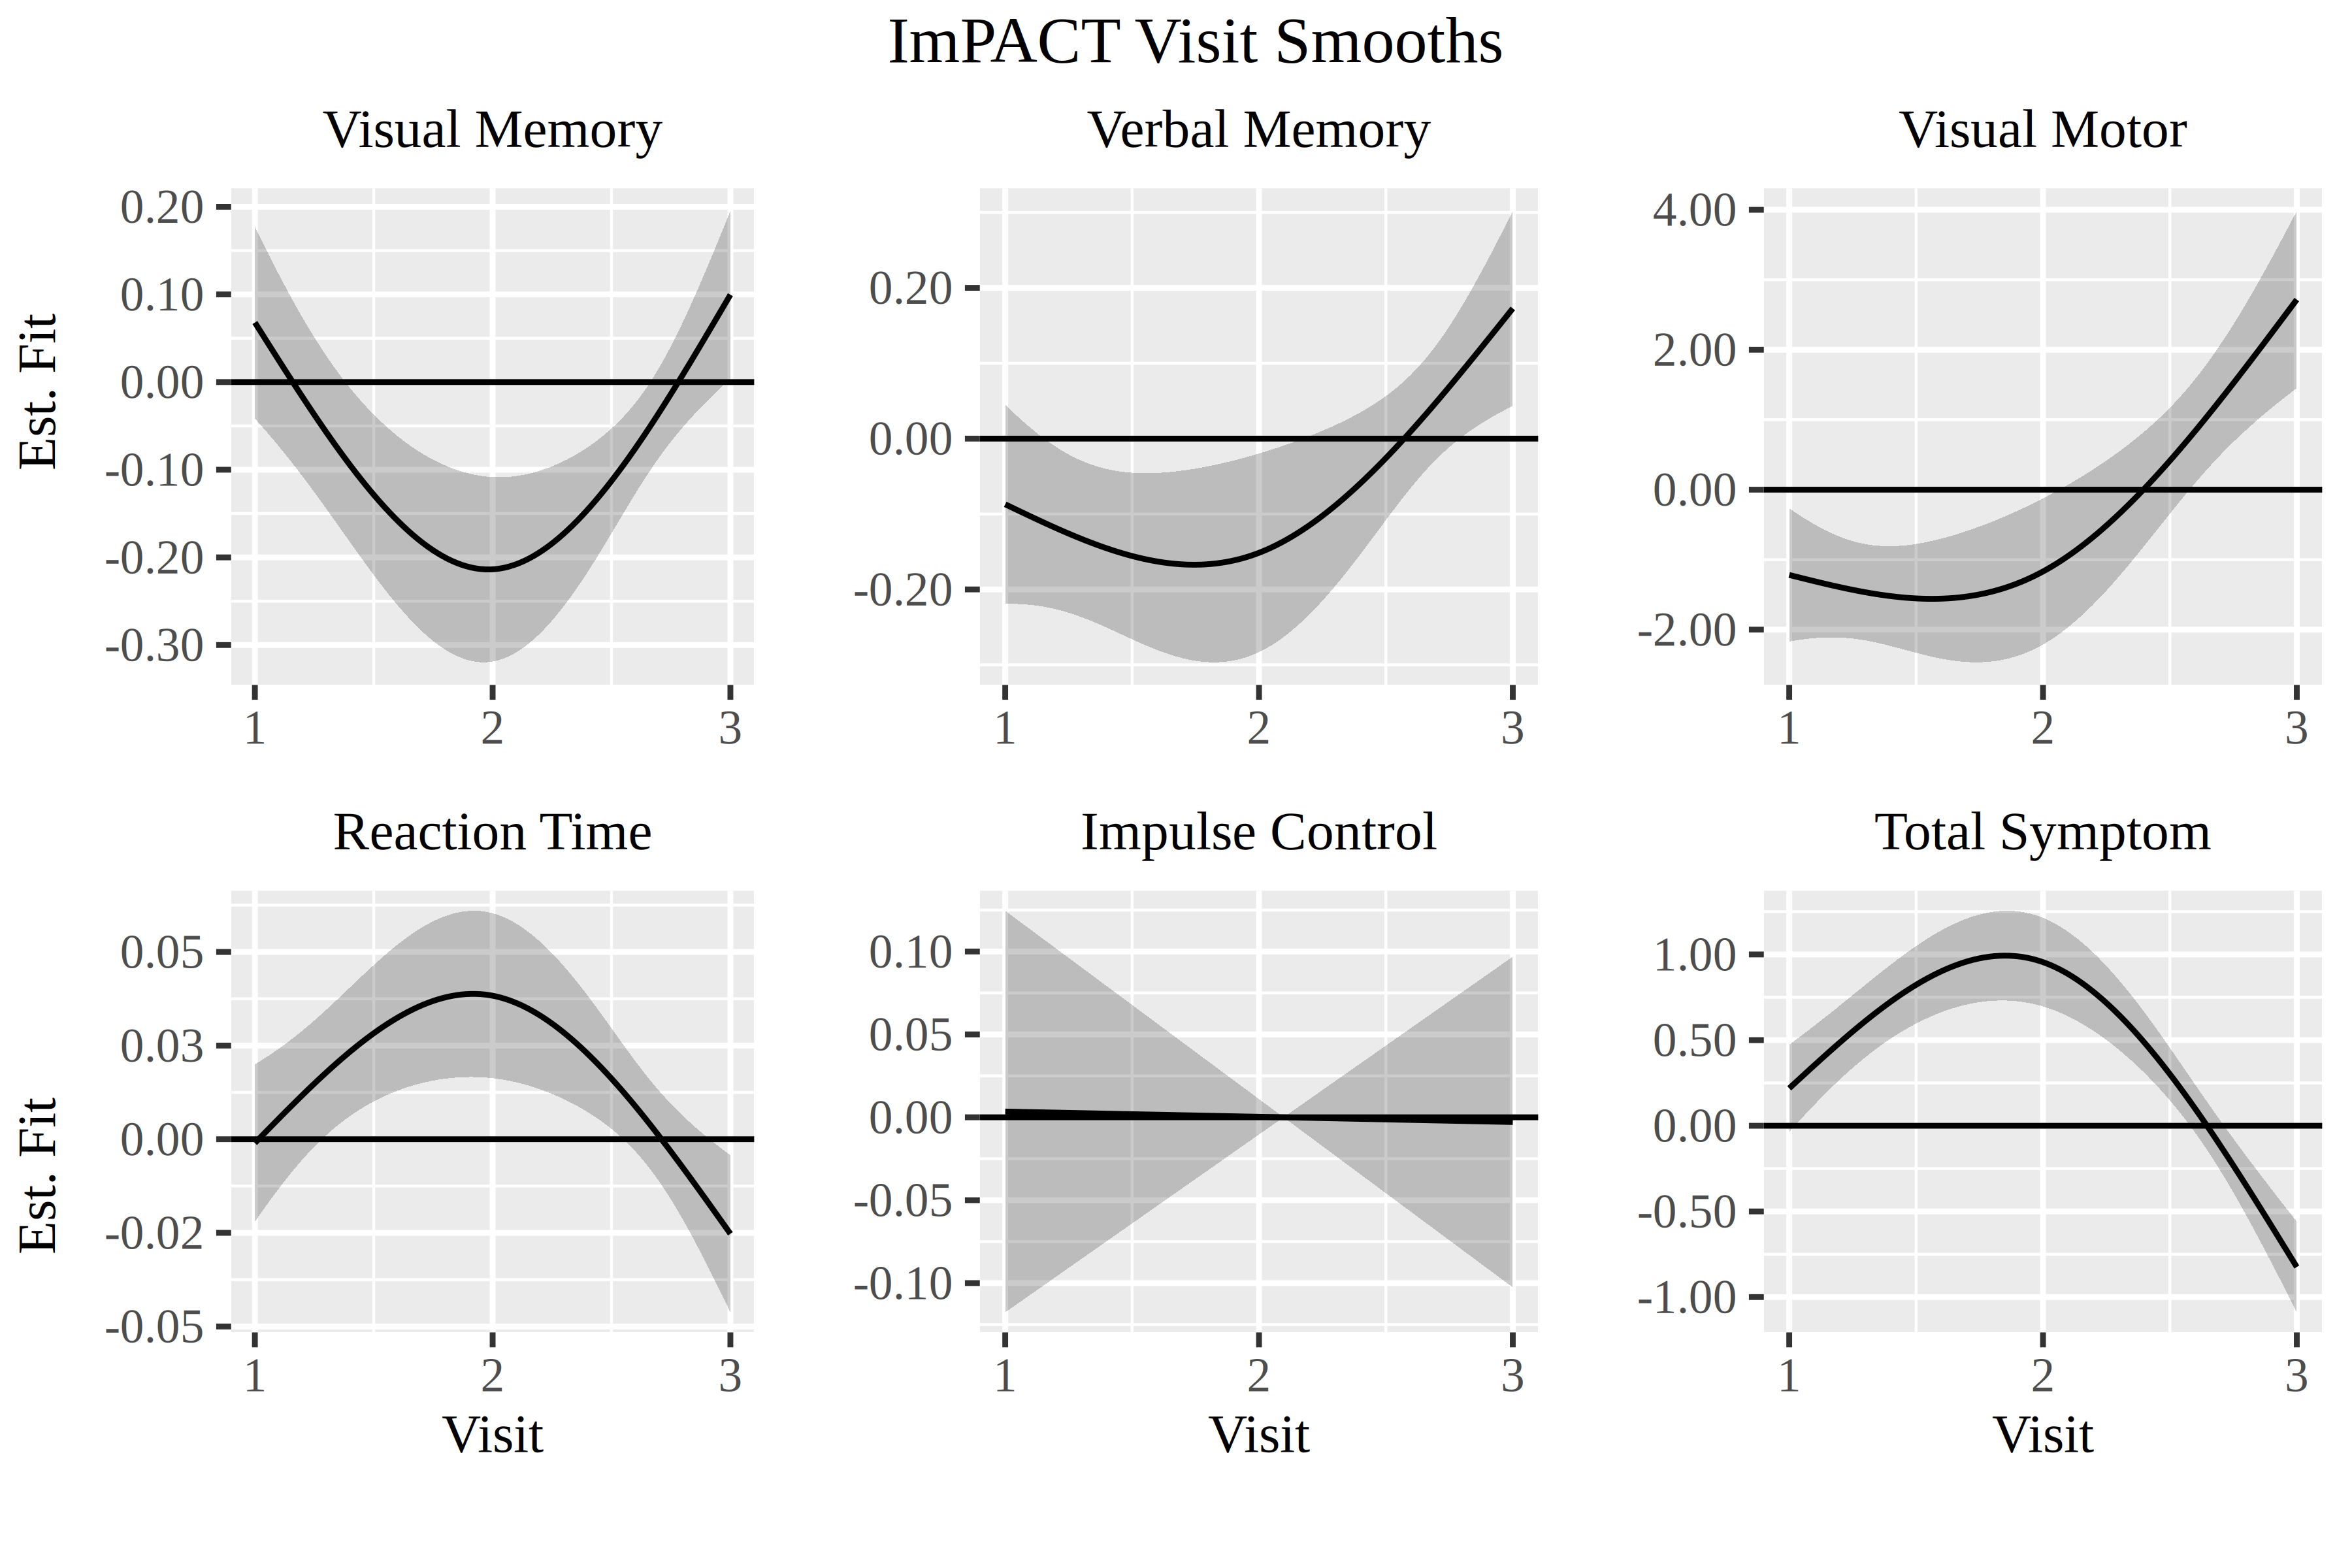
\includegraphics[width=0.7\textwidth]{fit_impact_gam.png}}
	\captionsetup{margin={0mm,0cm}}
	\caption{\textbf{(a)} Boxplots of ImPACT composite and total symptom scores, organized by visit. \textbf{(b)} GAM smooths for ImPACT composite and total symptom scores. Visits where the credible interval does not include 0 indicate significant change. Visual memory, reaction time, and total symptoms showed worsening and then recovery (U-shapes) while verbal memory and visual motor speed scores were better at assessment 3. Impulse control did not change across visits. Visit 1=Base, 2=Post, 3=RTP.}
	\label{fig:imp-gam}
\end{figure}


\subsection{Longitudinal Whole-Brain Analysis Detects Injury to Posterior Callosum}
\label{ssec:res-dwi-wba}
The longitudinal, whole-brain difference model (Section \ref{sssec:meth-gam-ldi}) produced tract difference smooths for Post vs. Base and RTP vs. Base $\Delta$FA values (Figure \ref{fig:ldi-gam}, top and middle). Surprisingly, test statistics for all smooths indicated significant non-flatness, indicating that each tract had visit differences from Base (Table \ref{tbl:ldi-gam}). We note that in interpreting GAM coefficients, the magnitude of the effect is equally relevant to the test statistic of non-flatness (F-stat). For instance, when interpreting Figure \ref{fig:ldi-gam}, the callosum orbital (CCorb, green) had a much larger magnitude compared to callosum temporal (CCtemp, pink) despite both tracts having equivalent `significance'. Nevertheless, it is well established that concussion is associated with negative diagnostic readings \parencite[e.g.][]{klein2019PrevalencePotentiallyClinically}, and we expected to only find changes to scalar values in regions commonly associated with traumatic axonal injury e.g. tracts which decussate through the splenium (here the superior parietal and posterior parietal callosal tracts).

\begin{figure}[H]
	\centering
	\fbox{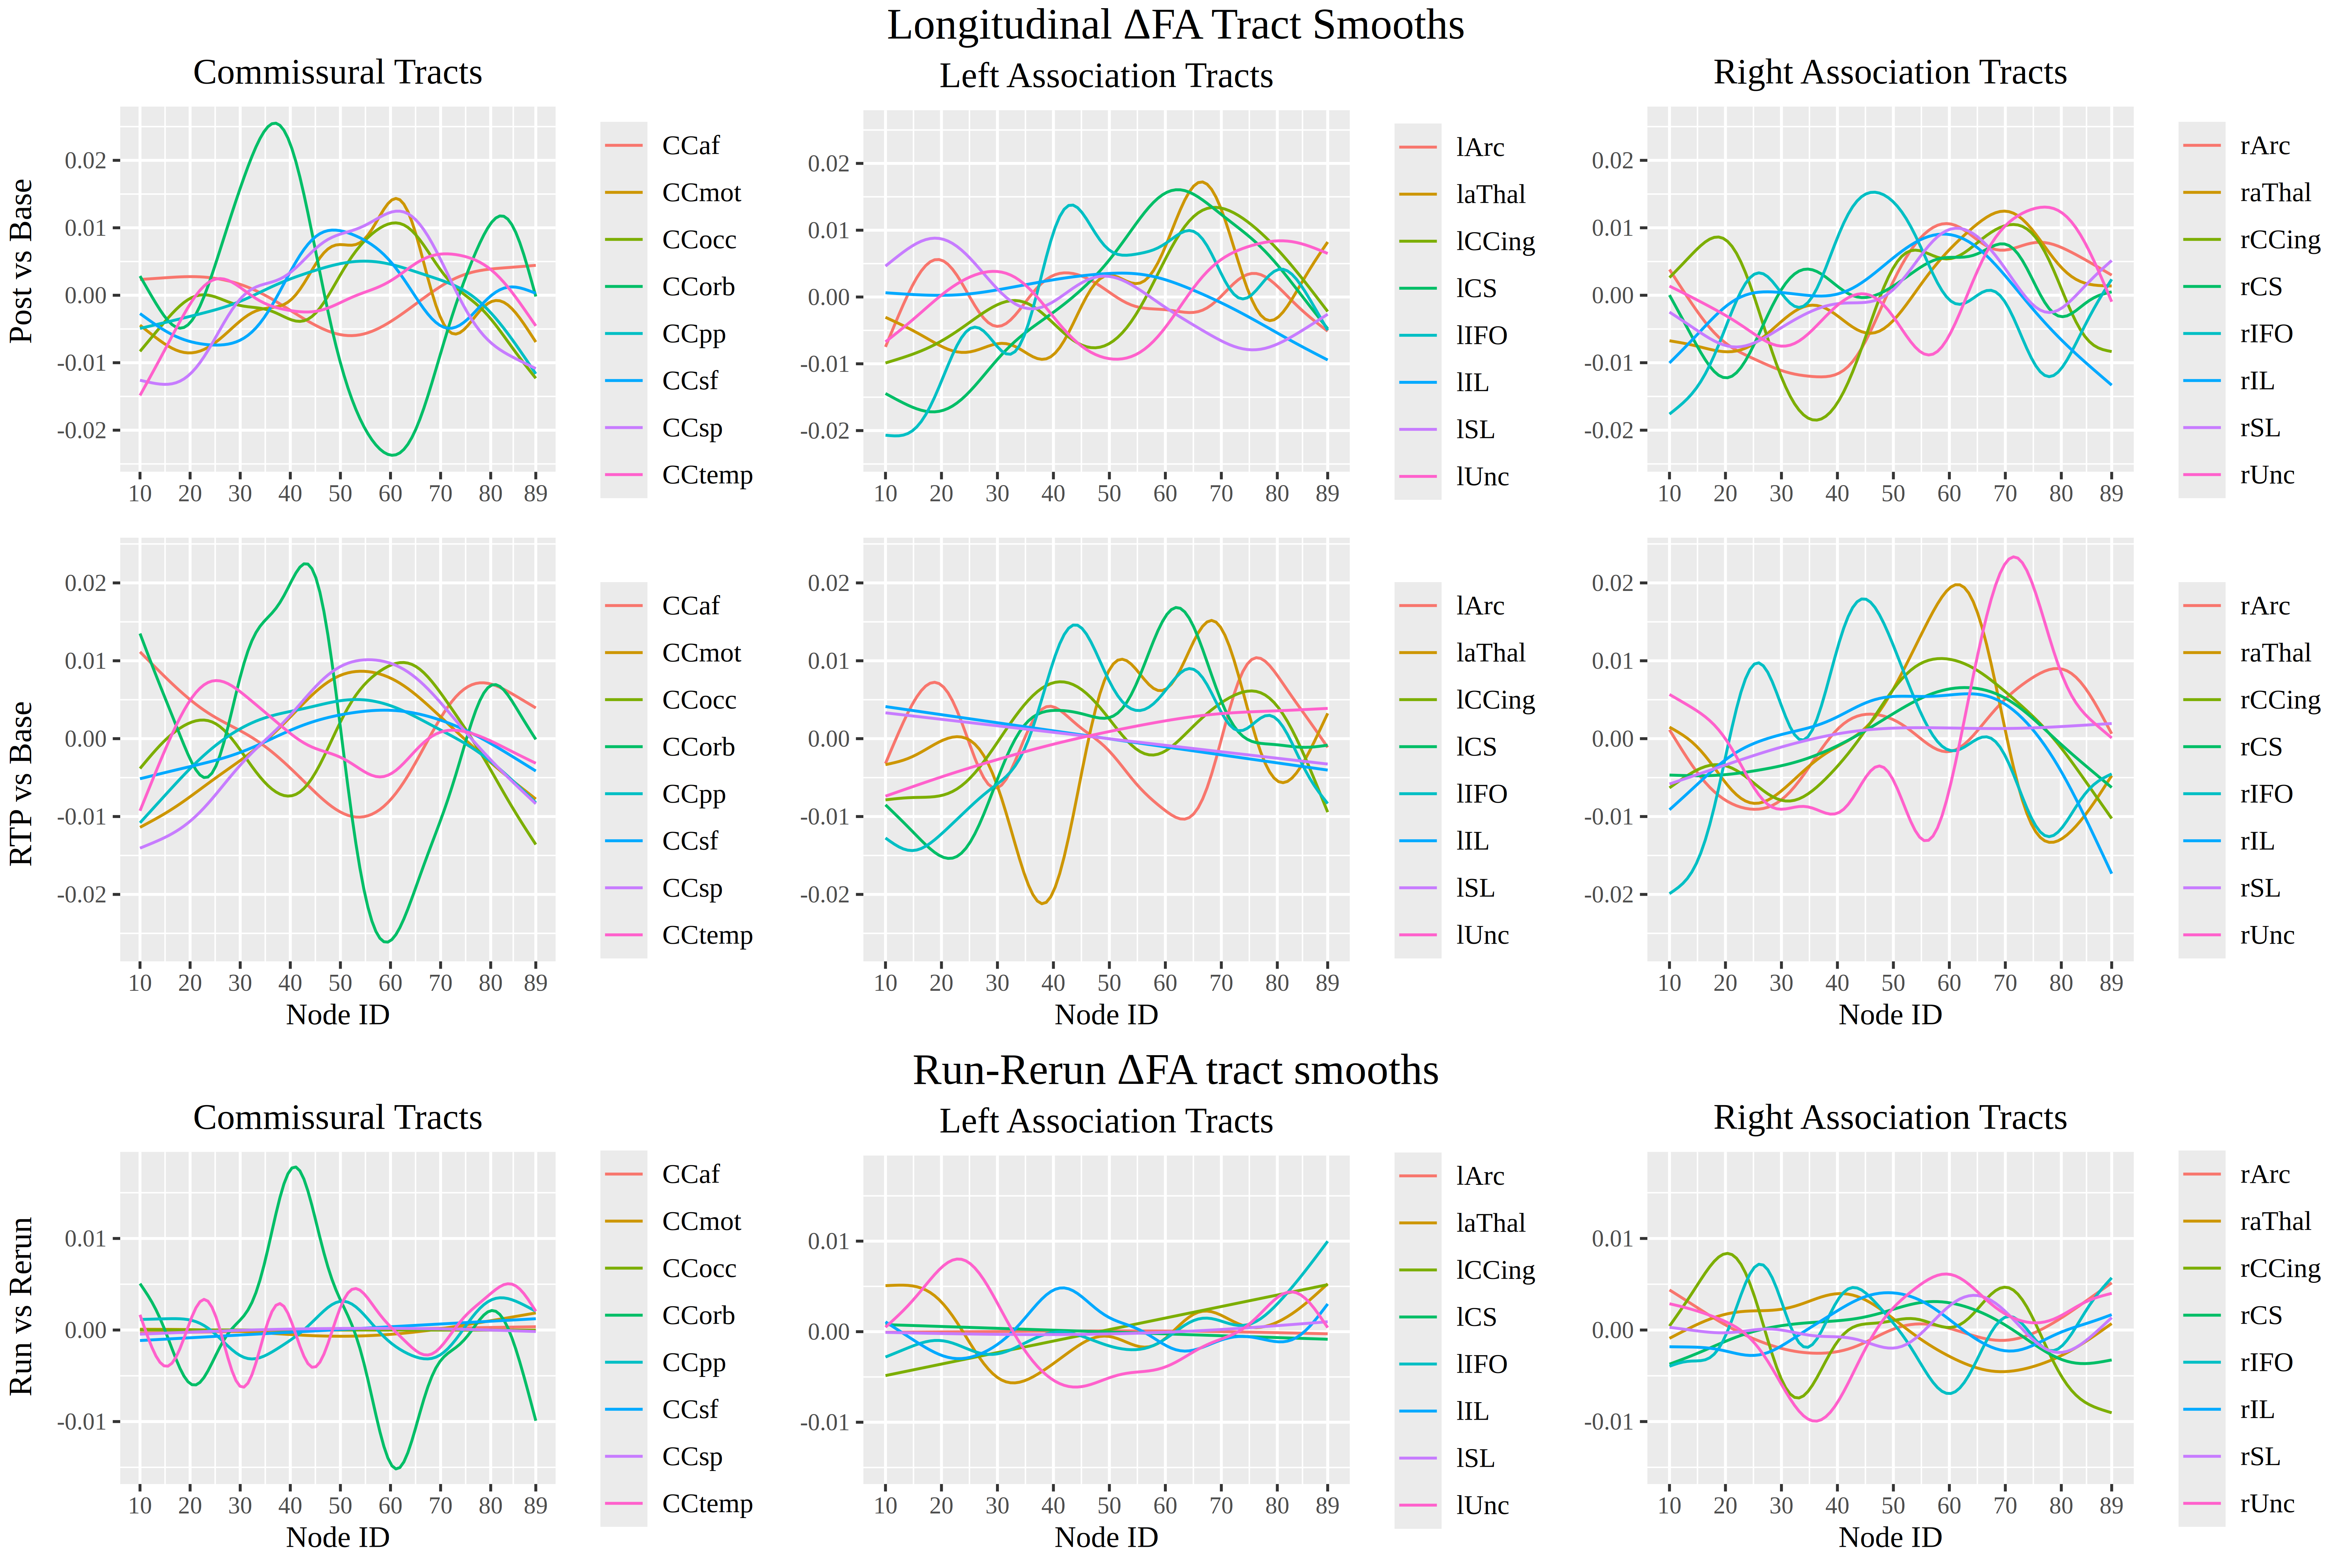
\includegraphics[width=0.95\textwidth]{fig_LDI_DI_rerun.png}}
	\caption{HGAM smooths of tract FA differences by node for comparisons against Base (top, middle) and Run vs. Rerun (bottom). \textbf{Top}: $\Delta$FA-Node smooths of Post relative to Base, deflections from zero here may be indicative of concussion-related changes. \textbf{Middle}: $\Delta$FA-Node smooths of RTP relative to Base, smaller deflections here than Post vs. Base may be indicative of recovery-related changes (and the converse for greater deflections). \textbf{Bottom}: $\Delta$FA-Node smooths of Run vs. Rerun, indicative of algorithmic variance by tract. Node IDs are numbered in the RAS convention, with midline of commissural fibers at node 50. Left: Corpus callosum tracts, middle: left hemisphere tracts, right: right hemisphere tracts. Credible intervals were omitted for visual clarity. \textit{Commissural tracts}: CCaf = anterior forceps, CCmot = motor, CCocc = occipital, CCorb = orbital, CCpp = posterior parietal, CCsf = superior frontal, CCsp = superior parietal, CCtemp = temporal. \textit{Association tracts}: Arc = arcuate, aThal = anterior thalamic, CCing = cingulum (cingulate portion), CS = corticospinal, IFO = inferior fronto-occipital, IL = inferior lateral, SL = superior lateral, Unc = uncinate; association tract acronyms are preceded by `l'/`r' to designate left/right hemisphere.}
	\label{fig:ldi-gam}
\end{figure}

As tractometry was conducted on each visit via PyAFQ, one potential source of variance is algorithmic run-rerun (test-retest) stability \parencite{wang2011LongitudinalChangesStructural}, particularly given our use of probabilistic tractography. Previous work has demonstrated high test-retest reliability metrics for PyAFQ \parencite{kruper2021EvaluatingReliabilityHuman}, which also noted tract-dependent reliability metrics that averaged around 86\%. We note that concussion-related scalar changes may not be as large as 14\%, particularly at the group level due to injury heterogeneity. Nevertheless, we reran tractography on the Base visit and calculated Run vs. Rerun $\Delta$FA values for each subject's tract profiles to quantify the amount of algorithmic variance in our data. The Run vs. Rerun $\Delta$FA were modeled with a non-longitudinal variant of R Code \ref{code:gam-ldi} (Supplemental R Code \ref{supp-code:gam-di}). Resulting smooths (Figure \ref{fig:ldi-gam}, bottom) illustrate the amount of algorithmic variance that can be expected for each tract, where some tracts have demonstrably high variance (e.g. callosum orbital, CCorb) while others are more stable (superior frontal callosum, CCsf). Importantly, corresponding test statistics identified a number of tracts which did not significantly differ between run and rerun (Table \ref{tbl:ldi-gam}, Run vs. Rerun): callosum anterior frontal (CCaf), callosum motor (CCmot), callosum occipital (CCocc), callosum superior parietal (CCsp), left arcuate (lArc), left corticospinal (lCS), and left superior longitudinal (lSL).

\begin{table}[H]
	\scriptsize
	% Please add the following required packages to your document preamble:
% \usepackage[table,xcdraw]{xcolor}
% Beamer presentation requires \usepackage{colortbl} instead of \usepackage[table,xcdraw]{xcolor}
\begin{tabular}{lllll|llll|llll}
 & \multicolumn{4}{c|}{Post-Base} & \multicolumn{4}{c|}{RTP-Base} & \multicolumn{4}{c}{Run-Rerun} \\ \cline{2-13}
Tract & \multicolumn{1}{c}{edf} & \multicolumn{1}{c}{Ref.df} & \multicolumn{1}{c}{F} & \multicolumn{1}{c|}{Sig} & \multicolumn{1}{c}{edf} & \multicolumn{1}{c}{Ref.df} & \multicolumn{1}{c}{F} & \multicolumn{1}{c|}{Sig} & \multicolumn{1}{c}{edf} & \multicolumn{1}{c}{Ref.df} & \multicolumn{1}{c}{F} & \multicolumn{1}{c}{Sig} \\ \hline
\multicolumn{1}{l|}{CCaf} & 4.58 & 5.70 & 5.52 & \textbf{***} & 5.82 & 7.20 & 11.90 & \textbf{***} & 1.00 & 1.00 & 0.34 & \textbf{} \\
\rowcolor[HTML]{C0C0C0}
\multicolumn{1}{l|}{\cellcolor[HTML]{C0C0C0}CCmot} & 9.63 & 11.43 & 9.89 & \textbf{***} & 4.34 & 5.41 & 15.23 & \textbf{***} & 2.27 & 2.83 & 1.84 & \textbf{} \\
\multicolumn{1}{l|}{CCocc} & 7.13 & 8.74 & 9.12 & \textbf{***} & 6.79 & 8.35 & 9.53 & \textbf{***} & 1.00 & 1.01 & \cellcolor[HTML]{FFFFFF}0.00 & \textbf{} \\
\rowcolor[HTML]{C0C0C0}
\multicolumn{1}{l|}{\cellcolor[HTML]{C0C0C0}CCorb} & 9.71 & 11.50 & 30.92 & \textbf{***} & 10.56 & 12.28 & 28.06 & \textbf{***} & 12.01 & 13.35 & 36.29 & \textbf{***} \\
\multicolumn{1}{l|}{CCpp} & 4.35 & 5.42 & 7.62 & \textbf{***} & 3.78 & 4.71 & 9.10 & \textbf{***} & 8.01 & 9.74 & 4.43 & \textbf{***} \\
\rowcolor[HTML]{C0C0C0}
\multicolumn{1}{l|}{\cellcolor[HTML]{C0C0C0}CCsf} & 7.20 & 8.83 & 9.11 & \textbf{***} & 3.15 & 3.94 & 4.77 & \textbf{***} & 1.00 & 1.00 & 3.95 & \textbf{*} \\
\multicolumn{1}{l|}{CCsp} & 7.09 & 8.70 & 20.93 & \textbf{***} & 4.75 & 5.91 & 21.22 & \textbf{***} & 1.43 & 1.74 & 0.34 & \textbf{} \\
\rowcolor[HTML]{C0C0C0}
\multicolumn{1}{l|}{\cellcolor[HTML]{C0C0C0}CCtemp} & 6.40 & 7.89 & 6.61 & \textbf{***} & 6.32 & 7.80 & 4.43 & \textbf{***} & 12.31 & 13.52 & 6.23 & \textbf{***} \\
\multicolumn{1}{l|}{laThal} & 9.98 & 11.76 & 12.34 & \textbf{***} & 10.55 & 12.27 & 15.29 & \textbf{***} & 8.20 & 9.95 & 8.54 & \textbf{***} \\
\rowcolor[HTML]{C0C0C0}
\multicolumn{1}{l|}{\cellcolor[HTML]{C0C0C0}lArc} & 8.59 & 10.37 & 2.67 & \textbf{**} & 9.78 & 11.57 & 6.50 & \textbf{***} & 1.26 & 1.47 & 0.06 & \textbf{} \\
\multicolumn{1}{l|}{lCCing} & 7.17 & 8.79 & 15.00 & \textbf{***} & 6.96 & 8.55 & 6.98 & \textbf{***} & 1.00 & 1.00 & 70.30 & \textbf{***} \\
\rowcolor[HTML]{C0C0C0}
\multicolumn{1}{l|}{\cellcolor[HTML]{C0C0C0}lCS} & 6.41 & 7.90 & 37.00 & \textbf{***} & 8.88 & 10.67 & 15.25 & \textbf{***} & 1.00 & 1.00 & 1.82 & \textbf{} \\
\multicolumn{1}{l|}{lIFO} & 10.64 & 12.35 & 18.33 & \textbf{***} & 9.48 & 11.28 & 13.52 & \textbf{***} & 7.20 & 8.83 & 7.73 & \textbf{***} \\
\rowcolor[HTML]{C0C0C0}
\multicolumn{1}{l|}{\cellcolor[HTML]{C0C0C0}lIL} & 3.38 & 4.22 & 7.15 & \textbf{***} & 1.01 & 1.02 & 11.67 & \textbf{***} & 7.83 & 9.54 & 4.46 & \textbf{***} \\
\multicolumn{1}{l|}{lSL} & 6.58 & 8.11 & 8.14 & \textbf{***} & 1.00 & 1.01 & 7.67 & \textbf{***} & 1.61 & 1.99 & 0.88 & \textbf{} \\
\rowcolor[HTML]{C0C0C0}
\multicolumn{1}{l|}{\cellcolor[HTML]{C0C0C0}lUnc} & 6.45 & 7.95 & 10.78 & \textbf{***} & 2.00 & 2.50 & 10.26 & \textbf{***} & 8.57 & 10.34 & 15.05 & \textbf{***} \\
\multicolumn{1}{l|}{raThal} & 7.32 & 8.97 & 12.45 & \textbf{***} & 9.06 & 10.86 & 17.64 & \textbf{***} & 5.68 & 7.04 & 9.47 & \textbf{***} \\
\rowcolor[HTML]{C0C0C0}
\multicolumn{1}{l|}{\cellcolor[HTML]{C0C0C0}rArc} & 7.33 & 8.97 & 17.97 & \textbf{***} & 6.94 & 8.53 & 7.59 & \textbf{***} & 5.41 & 6.71 & 5.30 & \textbf{***} \\
\multicolumn{1}{l|}{rCCing} & 9.41 & 11.21 & 18.11 & \textbf{***} & 6.07 & 7.50 & 11.80 & \textbf{***} & 10.61 & 12.33 & 14.86 & \textbf{***} \\
\rowcolor[HTML]{C0C0C0}
\multicolumn{1}{l|}{\cellcolor[HTML]{C0C0C0}rCS} & 8.95 & 10.75 & 6.66 & \textbf{***} & 4.17 & 5.19 & 7.53 & \textbf{***} & 5.18 & 6.43 & 6.69 & \textbf{***} \\
\multicolumn{1}{l|}{rIFO} & 10.10 & 11.87 & 15.38 & \textbf{***} & 10.60 & 12.31 & 16.69 & \textbf{***} & 11.49 & 13.01 & 8.77 & \textbf{***} \\
\rowcolor[HTML]{C0C0C0}
\multicolumn{1}{l|}{\cellcolor[HTML]{C0C0C0}rIL} & 5.74 & 7.10 & 12.47 & \textbf{***} & 4.99 & 6.20 & 11.56 & \textbf{***} & 6.18 & 7.63 & 5.82 & \textbf{***} \\
\multicolumn{1}{l|}{rSL} & 7.32 & 8.97 & 7.52 & \textbf{***} & 2.30 & 2.87 & 3.64 & \textbf{*} & 7.45 & 9.11 & 2.92 & \textbf{**} \\
\rowcolor[HTML]{C0C0C0}
\multicolumn{1}{l|}{\cellcolor[HTML]{C0C0C0}rUnc} & 8.43 & 10.19 & 11.34 & \textbf{***} & 10.18 & 11.94 & 18.80 & \textbf{***} & 8.62 & 10.40 & 16.32 & \textbf{***}
\end{tabular}

	\caption{Longitudinal whole-brain HGAM statistics for tract smooths. Significant non-flatness was detected for all difference smooths in the longitudinal concussion model (Post vs. Base, RTP vs. Base), and a number of tracts did not show significant differences between multiple runs of the tractography pipeline (Run vs. Rerun) e.g. CCsp. Post vs. Base = FA difference between Post and Base, RTP vs. Base = FA difference between RTP and Base, Run vs. Rerun = FA difference between multiple runs of PyAFQ. edf = effective degrees of freedom, F = F-statistic, Sig = significance. *** = p$<$.001, ** = p$<$.01, * = p$<$.05. See Figure \ref{fig:ldi-gam} for tract names.}
	\label{tbl:ldi-gam}
\end{table}

To test our first hypothesis that concussion injury- and recovery-related changes would be evident in posterior callosal FA values, we compared the smooths' statistic, magnitude of effect, and credible intervals from both the whole-brain longitudinal and run-rerun models. Taken together, we found evidence that partially supports our hypothesis: the callosum superior parietal Post vs. Base smooth from the longitudinal whole-brain model showed significant FA differences while the run-rerun model did not, which we interpreted as evidence of concussion injury-related changes. The RTP vs. Base smooth, however, also differed significantly, and accordingly we did not detect evidence of recovery (also, see Section \ref{sssec:res-dwi-pat-norecov}). Further, the Post and RTP vs. Base differences detected in the callosum posterior parietal whole-brain longitudinal smooth did not have magnitudes greater than the run-rerun smooth, suggesting that the detected differences may be due to algorithmic- and not necessarily concussion-related variance.


\subsection{Tract Injuries Precede Recovery, Progression, or No Change}
\label{ssec:res-dwi-pat}
As all tracts were modeled in a single, whole-brain longitudinal model in order to account for within-subject variance, we additionally investigated the other tract smooths for concussion injury- and recovery-related FA changes that were above and beyond any variance explained by run-rerun model. This analysis identified three patterns of FA differences: injury and recovery, injury with subsequent progression, and injury without recovery. Specifically, (a) injury and recovery was detected in the callosum superior frontal and right cingulum cingulate, (b) evidence of injury and progression was found in the callosum superior parietal (as stated above), left corticospinal, right anterior thalamic, and right inferior fronto-occipital, and (c) and the callosum motor, callosum orbital, left arcuate, and right uncinate tracts showed injury without subsequent change.

For each of these identified tracts, we conducted post-hoc models of FA, MD, AD, and RD in order to interrogate the source of FA changes, testing for Post and RTP differences from Base (R Code \ref{code:gam-lgio}). Such models are necessary as AD ($\lambda_\parallel$) \textit{or} RD ($\lambda_\perp$) can drive FA differences, and are themselves related to different injury sequelae. These models tested our second hypothesis, that changes in FA are driven by RD and not AD. Additionally, where $\Delta$FA calculations require data at both visits for subtraction, these tract- and scalar-specific longitudinal models had a reduced factor structure which allowed us to predict scalar values, rather than scalar differences, thereby increasing the number of participants in the model (see Table \ref{tbl:meth-demo}).

Resulting test statistics (Table \ref{tbl:lgio-gam-tract}) indicated significant non-flatness across the majority of tracts and scalars, and a detailed description of these smooths is provided below. We note that the left arcuate FA at Post relative to Base is flat but becomes non-flat by RTP, indicative of late-emerging sequelae. Also, the AD smooths of the left corticospinal tract are flat relative to Base, indicating that nearly all the change in FA is driven by RD. For full interpretation, however, review of the partial effect smooths is needed to identify both the location (node) and direction of change.

\begin{table}[H]
	\tiny
	% Please add the following required packages to your document preamble:
% \usepackage{multirow}
% \usepackage[table,xcdraw]{xcolor}
% Beamer presentation requires \usepackage{colortbl} instead of \usepackage[table,xcdraw]{xcolor}

\begin{tabular}{llll|ll|ll|ll}
 &  & \multicolumn{2}{c|}{FA} & \multicolumn{2}{c|}{MD} & \multicolumn{2}{c|}{AD} & \multicolumn{2}{c}{RD} \\ \cline{3-10}
Tract & Smooth & \multicolumn{1}{c}{edf} & \multicolumn{1}{c|}{F} & \multicolumn{1}{c}{edf} & \multicolumn{1}{c|}{F} & \multicolumn{1}{c}{edf} & \multicolumn{1}{c|}{F} & \multicolumn{1}{c}{edf} & \multicolumn{1}{c}{F} \\ \hline
 & \multicolumn{1}{l|}{Global} & 13.96 & 2750.34 & 13.29 & 256.90 & 13.96 & 4077.09 & 13.83 & 636.96 \\
 & \multicolumn{1}{l|}{\cellcolor[HTML]{C0C0C0}O.Post} & \cellcolor[HTML]{C0C0C0}8.21 & \cellcolor[HTML]{C0C0C0}9.66 & \cellcolor[HTML]{C0C0C0}9.46 & \cellcolor[HTML]{C0C0C0}12.01 & \cellcolor[HTML]{C0C0C0}6.94 & \cellcolor[HTML]{C0C0C0}3.76 & \cellcolor[HTML]{C0C0C0}8.95 & \cellcolor[HTML]{C0C0C0}11.00 \\
\multirow{-3}{*}{CCsp} & \multicolumn{1}{l|}{O.RTP} & 8.10 & 11.02 & 9.30 & 12.57 & 6.29 & 3.02 & 9.04 & 11.67 \\
\rowcolor[HTML]{EFEFEF}
\cellcolor[HTML]{EFEFEF} & \multicolumn{1}{l|}{\cellcolor[HTML]{EFEFEF}Global} & 13.95 & 582.48 & 13.80 & 2762.05 & 13.97 & 4854.79 & 13.82 & 513.35 \\
\rowcolor[HTML]{C0C0C0}
\cellcolor[HTML]{EFEFEF} & \multicolumn{1}{l|}{\cellcolor[HTML]{C0C0C0}O.Post} & 8.99 & 4.70 & 6.23 & 2.68 & 6.29 & 1.14 & 8.53 & 5.78 \\
\rowcolor[HTML]{EFEFEF}
\multirow{-3}{*}{\cellcolor[HTML]{EFEFEF}CCsf} & \multicolumn{1}{l|}{\cellcolor[HTML]{EFEFEF}O.RTP} & 7.01 & 3.51 & 8.33 & 6.03 & 6.97 & 1.81 & 7.71 & 5.81 \\
\rowcolor[HTML]{FFFFFF}
\cellcolor[HTML]{FFFFFF} & \multicolumn{1}{l|}{\cellcolor[HTML]{FFFFFF}Global} & 13.95 & 538.33 & 13.86 & 3284.55 & 13.98 & 5804.04 & 13.62 & 501.66 \\
\rowcolor[HTML]{C0C0C0}
\cellcolor[HTML]{FFFFFF} & \multicolumn{1}{l|}{\cellcolor[HTML]{C0C0C0}O.Post} & 8.88 & 4.34 & 8.91 & 6.27 & 6.37 & 2.00 & 8.91 & 4.87 \\
\rowcolor[HTML]{FFFFFF}
\multirow{-3}{*}{\cellcolor[HTML]{FFFFFF}CCmot} & \multicolumn{1}{l|}{\cellcolor[HTML]{FFFFFF}O.RTP} & 8.41 & 8.05 & 8.72 & 8.74 & 6.41 & 1.26 & 8.28 & 8.54 \\
\rowcolor[HTML]{EFEFEF}
\cellcolor[HTML]{EFEFEF} & \multicolumn{1}{l|}{\cellcolor[HTML]{EFEFEF}Global} & 13.01 & 500.23 & 10.65 & 94.12 & 12.52 & 549.89 & 12.27 & 94.55 \\
\rowcolor[HTML]{C0C0C0}
\cellcolor[HTML]{EFEFEF} & \multicolumn{1}{l|}{\cellcolor[HTML]{C0C0C0}O.Post} & 10.48 & 9.31 & 7.15 & 3.24 & 8.15 & 3.00 & 9.13 & 6.58 \\
\rowcolor[HTML]{EFEFEF}
\multirow{-3}{*}{\cellcolor[HTML]{EFEFEF}CCorb} & \multicolumn{1}{l|}{\cellcolor[HTML]{EFEFEF}O.RTP} & 11.47 & 12.39 & 11.92 & 16.88 & 10.86 & 11.00 & 11.95 & 16.50
\end{tabular}

	\caption{Tract-specific HGAM statistics for DWI scalars of select tracts. Separate models were conducted for each scalar of each tract, fitting both the global curvature and visit (Post, RTP) differences from Base. O.Post/RTP = Post/RTP group smooth as an ordered factor (relative to Base). edf = effective degrees of freedom, F = F-statistic, Sig = significance. *** = p$<$.001, ** = p$<$.01, * = p$<$.05. See Figure \ref{fig:ldi-gam} for tract names.}
	\label{tbl:lgio-gam-tract}
\end{table}


\subsubsection{Evidence of Injury and Recovery}
\label{sssec:res-dwi-pat-recov}
Longitudinal tract-specific scalar models identified patterns consistent with concussion injury- and recovery-related changes in the right cingulum cingulate (Figure \ref{fig:lgio-gam-recov}) and callosum superior frontal (Supplemental Figure \ref{supp-fig:lgio-gam-recov}). In the right cingulum cingulate, an FA decrease relative to Base is evident in the anterior portion of the Post smooth (nodes 30-40). This decrease is associated with an increased in RD in the same nodal region, and little-to-no difference in AD. Such a pattern is consistent with demyelination, which increases the relative ratio of free extracellular water to intercellular water. By RTP, RD and FA values for the same nodal region return to near Base values, seemingly indicative of partial recovery, in accordance with our second hypothesis.

\begin{figure}[H]
	\centering
	\fbox{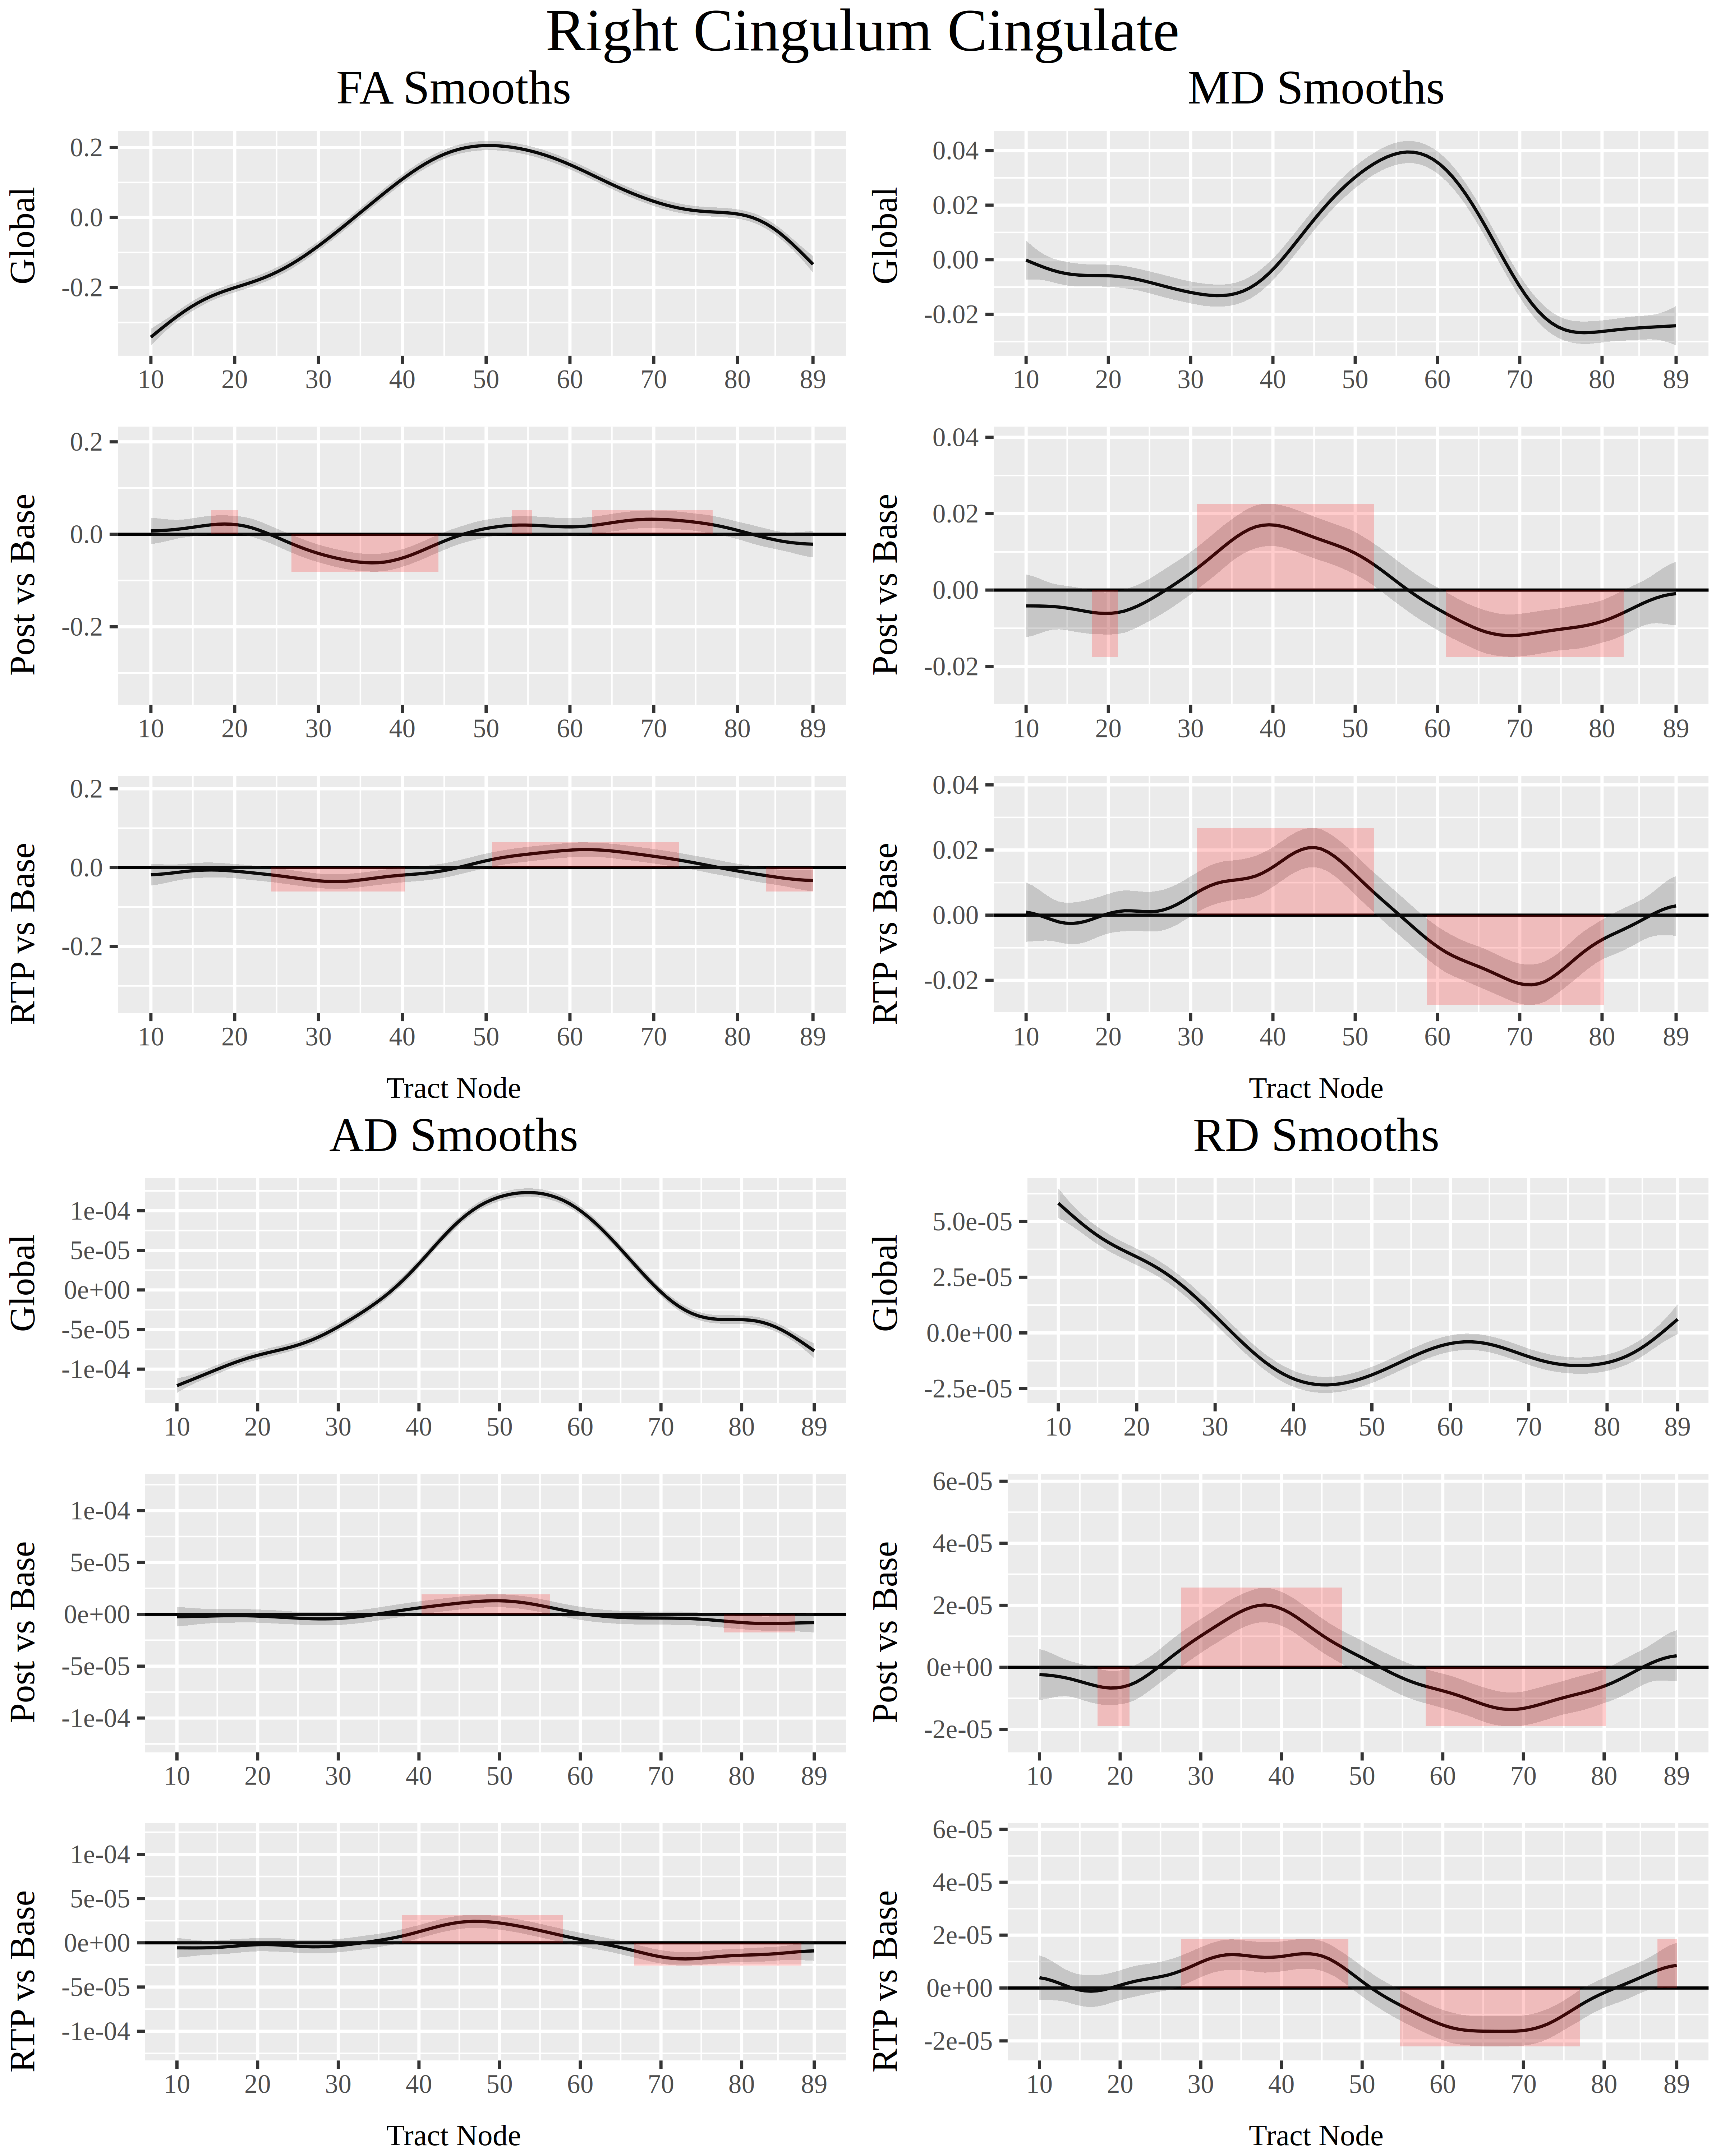
\includegraphics[width=.8\linewidth]{fit_LGIO_rCCing.png}}
	\caption{Longitudinal HGAM smooths modeling right cingulum cingulate scalars as a function of node and visit. Evidence of injury and recovery is detected about node 35 of the FA smooths, where significant decline is evident at Post relative to Base, the magnitude of which decreases by RTP. RD, and not AD, appear as the source of FA change. Red boxes indicate nodes where the credible intervals do not contain zero. Visit smooths are plotted in the domain of the global smooth to show their fit contribution. Nodes are numbered in RAS convention.}
	\label{fig:lgio-gam-recov}
\end{figure}

Further, these scalar smooths also show a different pattern in posterior regions of the tract (nodes 60-70). At both Post and RTP, a small increase in FA is detected which corresponds to a decrease in RD. This pattern of scalar change would be consistent with cellular edema, where an increase in the ratio of intracellular to extracellular water results in increased tortuosity and a corresponding decrease in diffusion speed. Increased tortuosity would also explain the decreased AD at RTP. Finally, we note the late emerging increase in AD about node 45, where RTP has a larger deflection from Base than Post. Such a pattern may be indicative of glial scarring [CITE].

Similarly, within-tract FA changes in the callosum superior frontal (Supplemental Figure \ref{supp-fig:lgio-gam-recov}) are driven entirely by RD, as indicated by flat AD smooths. Midline increases in FA (about node 50) at Post are associated with decreased RD, and both FA and RD values return to near baseline values by RTP. This pattern is reversed in the right hemisphere (node 25), with decreased FA values being driven by increased RD. Together, these smooths reveal subtle, within-tract dynamics that vary both anatomically (anteroposterior or mediolateral) and temporally (Post or RTP relative to Base), and provide evidence that these concussion-related changes in FA are driven by RD.


\subsubsection{Evidence of Injury Progression}
\label{sssec:res-dwi-pat-prog}
Four tracts demonstrated patterns of FA change that are consistent with injury progression: the left arcuate (Figure \ref{fig:lgio-gam-prog}), callosum motor, callosum orbital, and right uncinate (Supplemental Figure \ref{supp-fig:lgio-gam-prog}). In reviewing the left arcuate FA smooths, it first appears that we did not detect any damage during the acute phase of the injury, as evidenced by the flat Post vs. Base smooth (also, Table \ref{tbl:lgio-gam-tract}), but instead detected FA decline which emerged during the chronic phase (RTP) about node 65. As above, this FA decrease is associated with RD increase in the same nodal region without accompanying changes in AD. Additionally, there appears slight increases in FA towards the tract's posterior end (nodes 80+) which also appear to align with RD decrease.

That said, we note the increases in both RD and AD (and MD) about node 30 during Post vs. Base. These deflections are interesting as they essentially counter-balance each other, yielding no statistical change in FA. These AD and RD results suggest that the anterior portion of the left arcuate was damaged at Post (relative to Base) and recovered by RTP. Had we only investigated FA values we would have failed to detect these subtle deflections, resulting in a Type-II error.

\begin{figure}[H]
	\centering
	\fbox{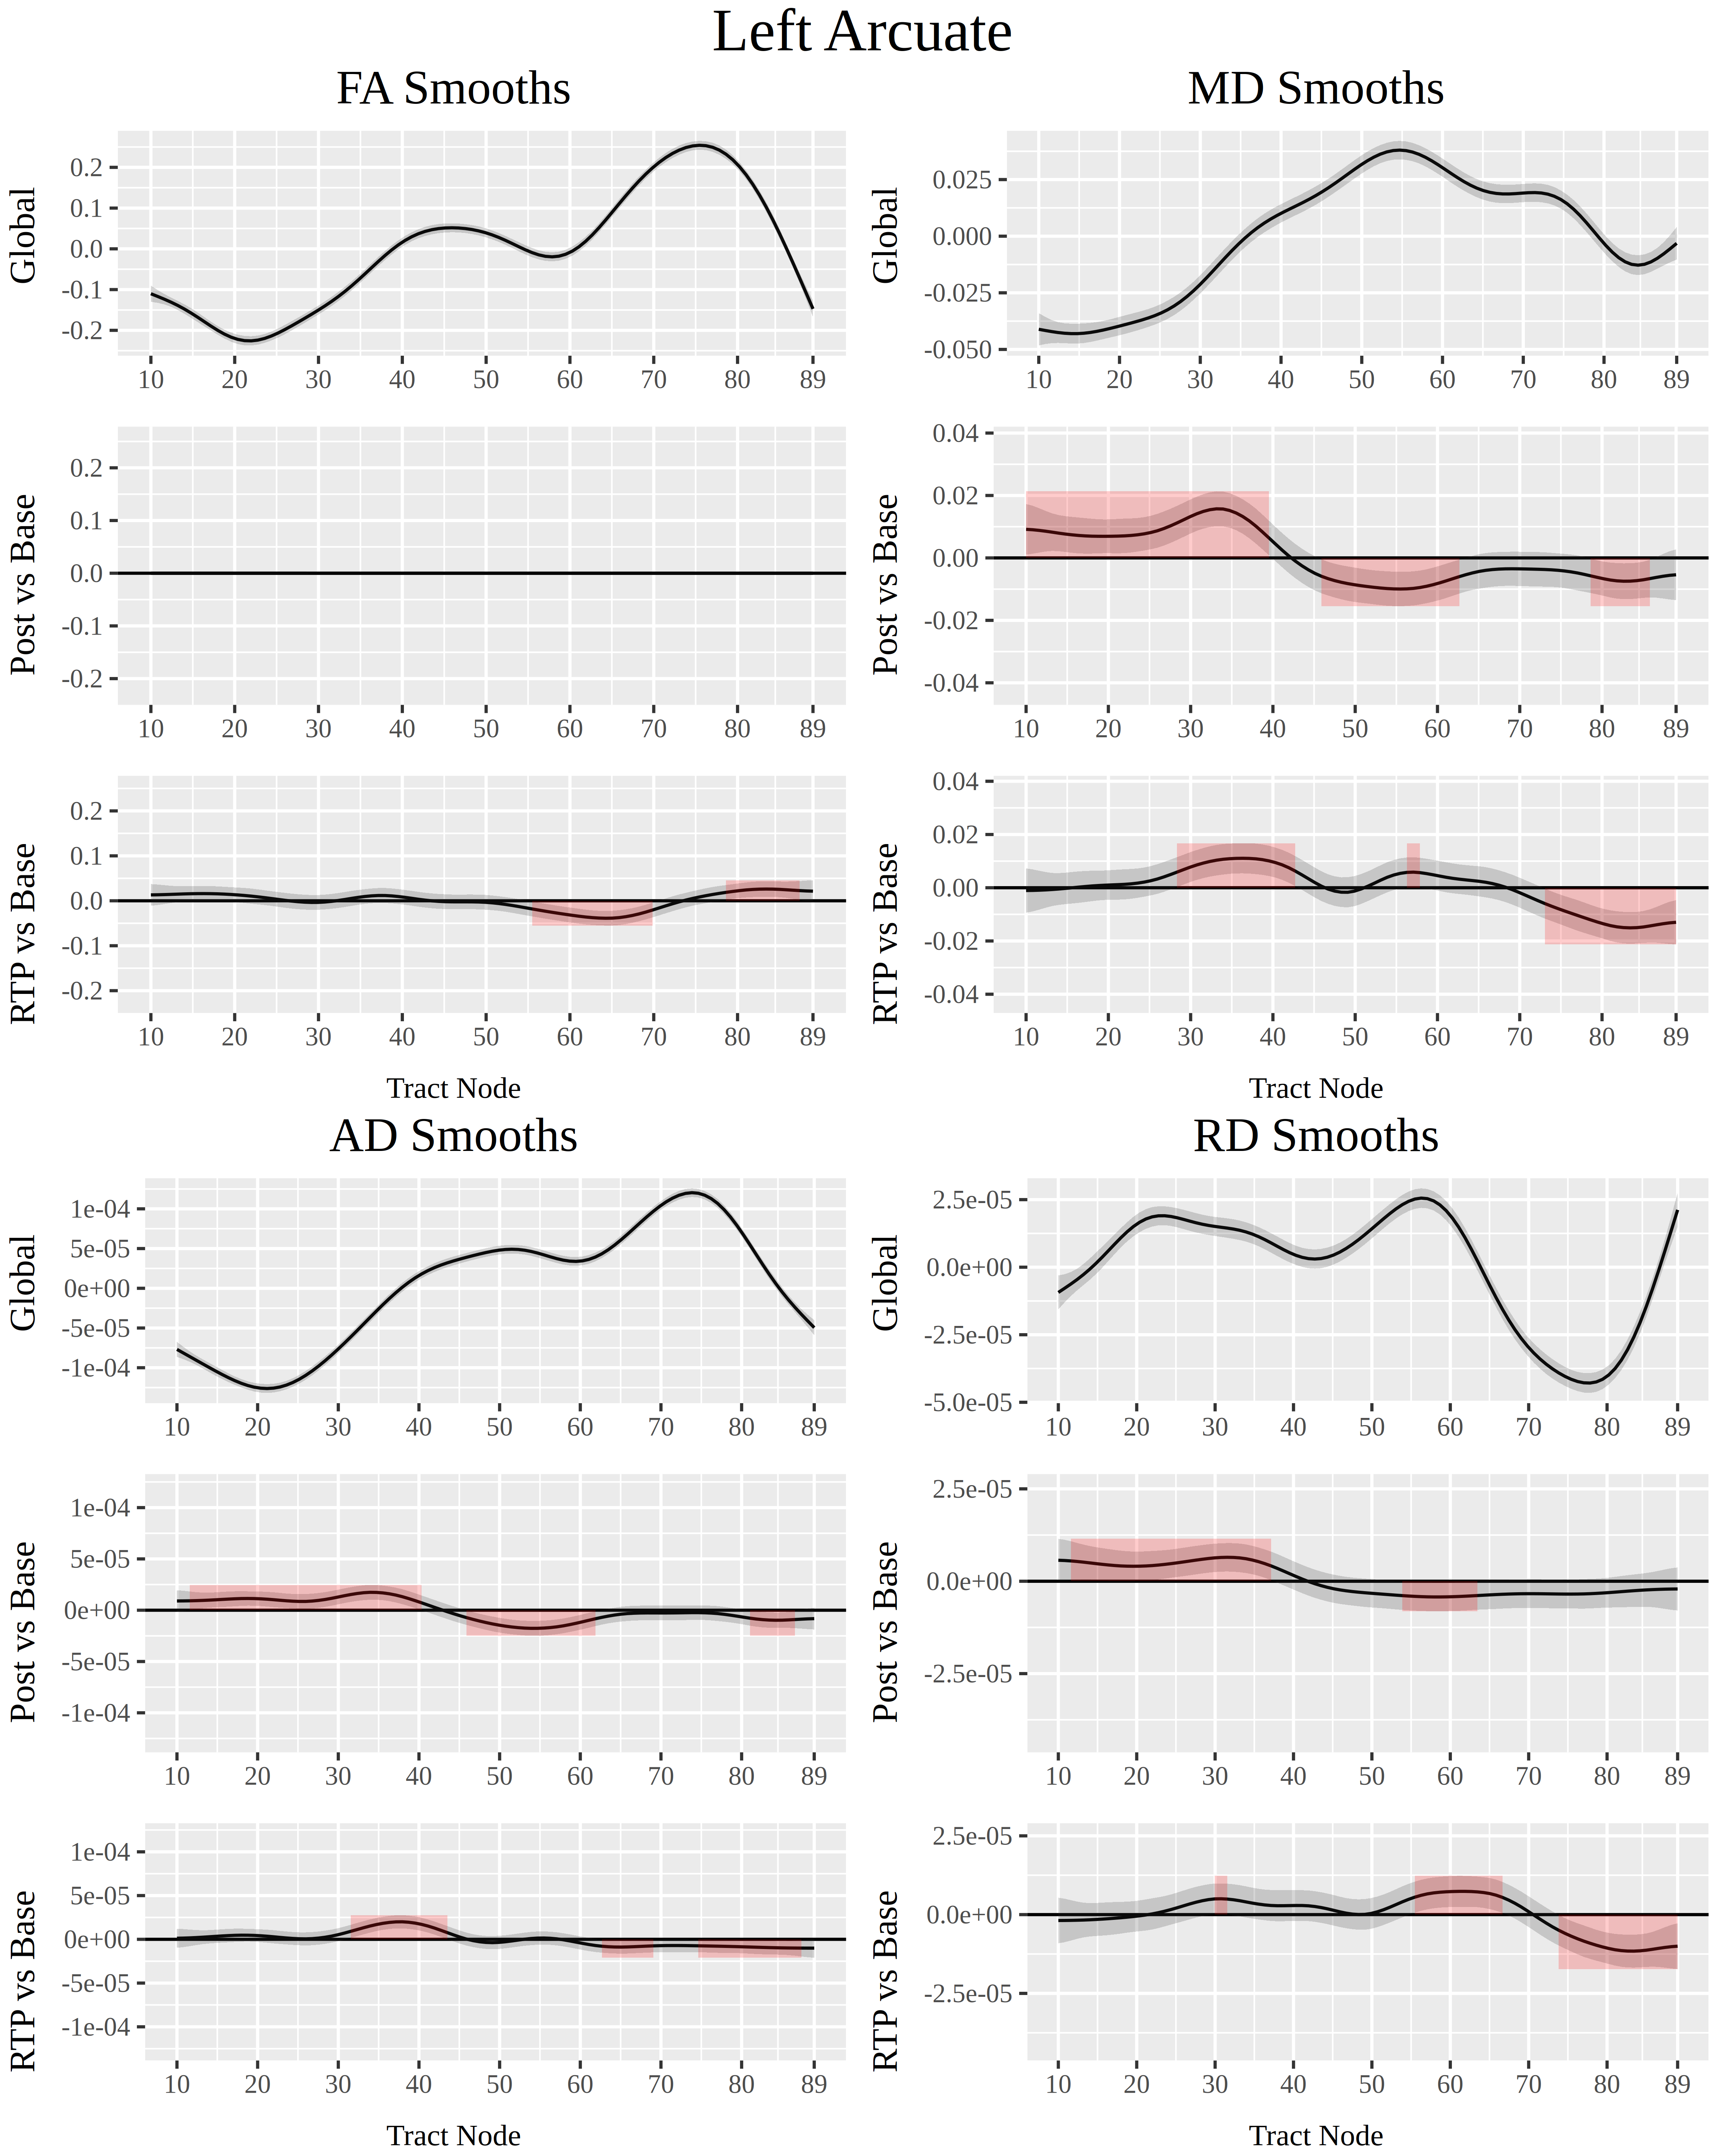
\includegraphics[width=.8\linewidth]{fit_LGIO_lArc.png}}
	\caption{Longitudinal HGAM smooths modeling left arcuate scalars as a function of node and visit. Evidence of late injury is detected in the RTP vs. Base FA smooth about node 65.}
	\label{fig:lgio-gam-prog}
\end{figure}

With respect to the remaining three tracts, two patterns emerge. First, we detected a similar pattern in the callosum orbital (Supplemental Figure \ref{supp-fig:lgio-gam-prog} b), where FA is strongly declined relative to Base at RTP (node 60). The majority of this FA decrease is driven by RD increase, as above, but we also detected late AD increase near the same region of the tract and extending towards node 40. Accordingly, these data suggest that the left and right portions of the callosum orbital tract have differing sequelae that do not necessarily resolve by return-to-play clearance.

Second, the callosum motor and right uncinate (Supplemental Figure \ref{supp-fig:lgio-gam-prog} a, c) both had FA increases by RTP in the left (callosal) and anterior (uncinate) portions of their tract (about nodes 60 and 70, respectively) which results from RD decrease in the same nodal region. For lower node values (right callosal, posterior uncinate), FA values were lower with respect to Base at both Post and RTP (nodes 20 and 40, respectively). These decreases in FA were driven by increased RD and, unlike the left arcuate and callosum orbital, we did not detect a change in AD values. These four tracts (and those reported below) provide evidence that even when athletes meet return-to-play criteria, long-term secondary injury considerations are still warranted and such criteria may not necessarily indicate that athletes are fully recovered.


\subsubsection{Evidence of Injury Without Recovery}
\label{sssec:res-dwi-pat-norecov}
In addition to patterns indicative of concussion-related injury preceding recovery or progression, we also detected injury preceding a lack of recovery in four tracts: callosum superior parietal (Figure \ref{fig:lgio-gam-norecov}), left corticospinal, right anterior thalamic, and right inferior fronto-occipital (Supplemental Figure \ref{supp-fig:lgio-gam-norecov}). In each of these tracts, an increase in FA was detected which corresponded to a decrease in RD in the same region. For instance, the callosum superior parietal Post vs. Base FA smooth revealed increased FA values about node 55, an increase which appears to be driven by a decrease in RD in the same region, and without change in AD.

\begin{figure}[H]
	\centering
	\fbox{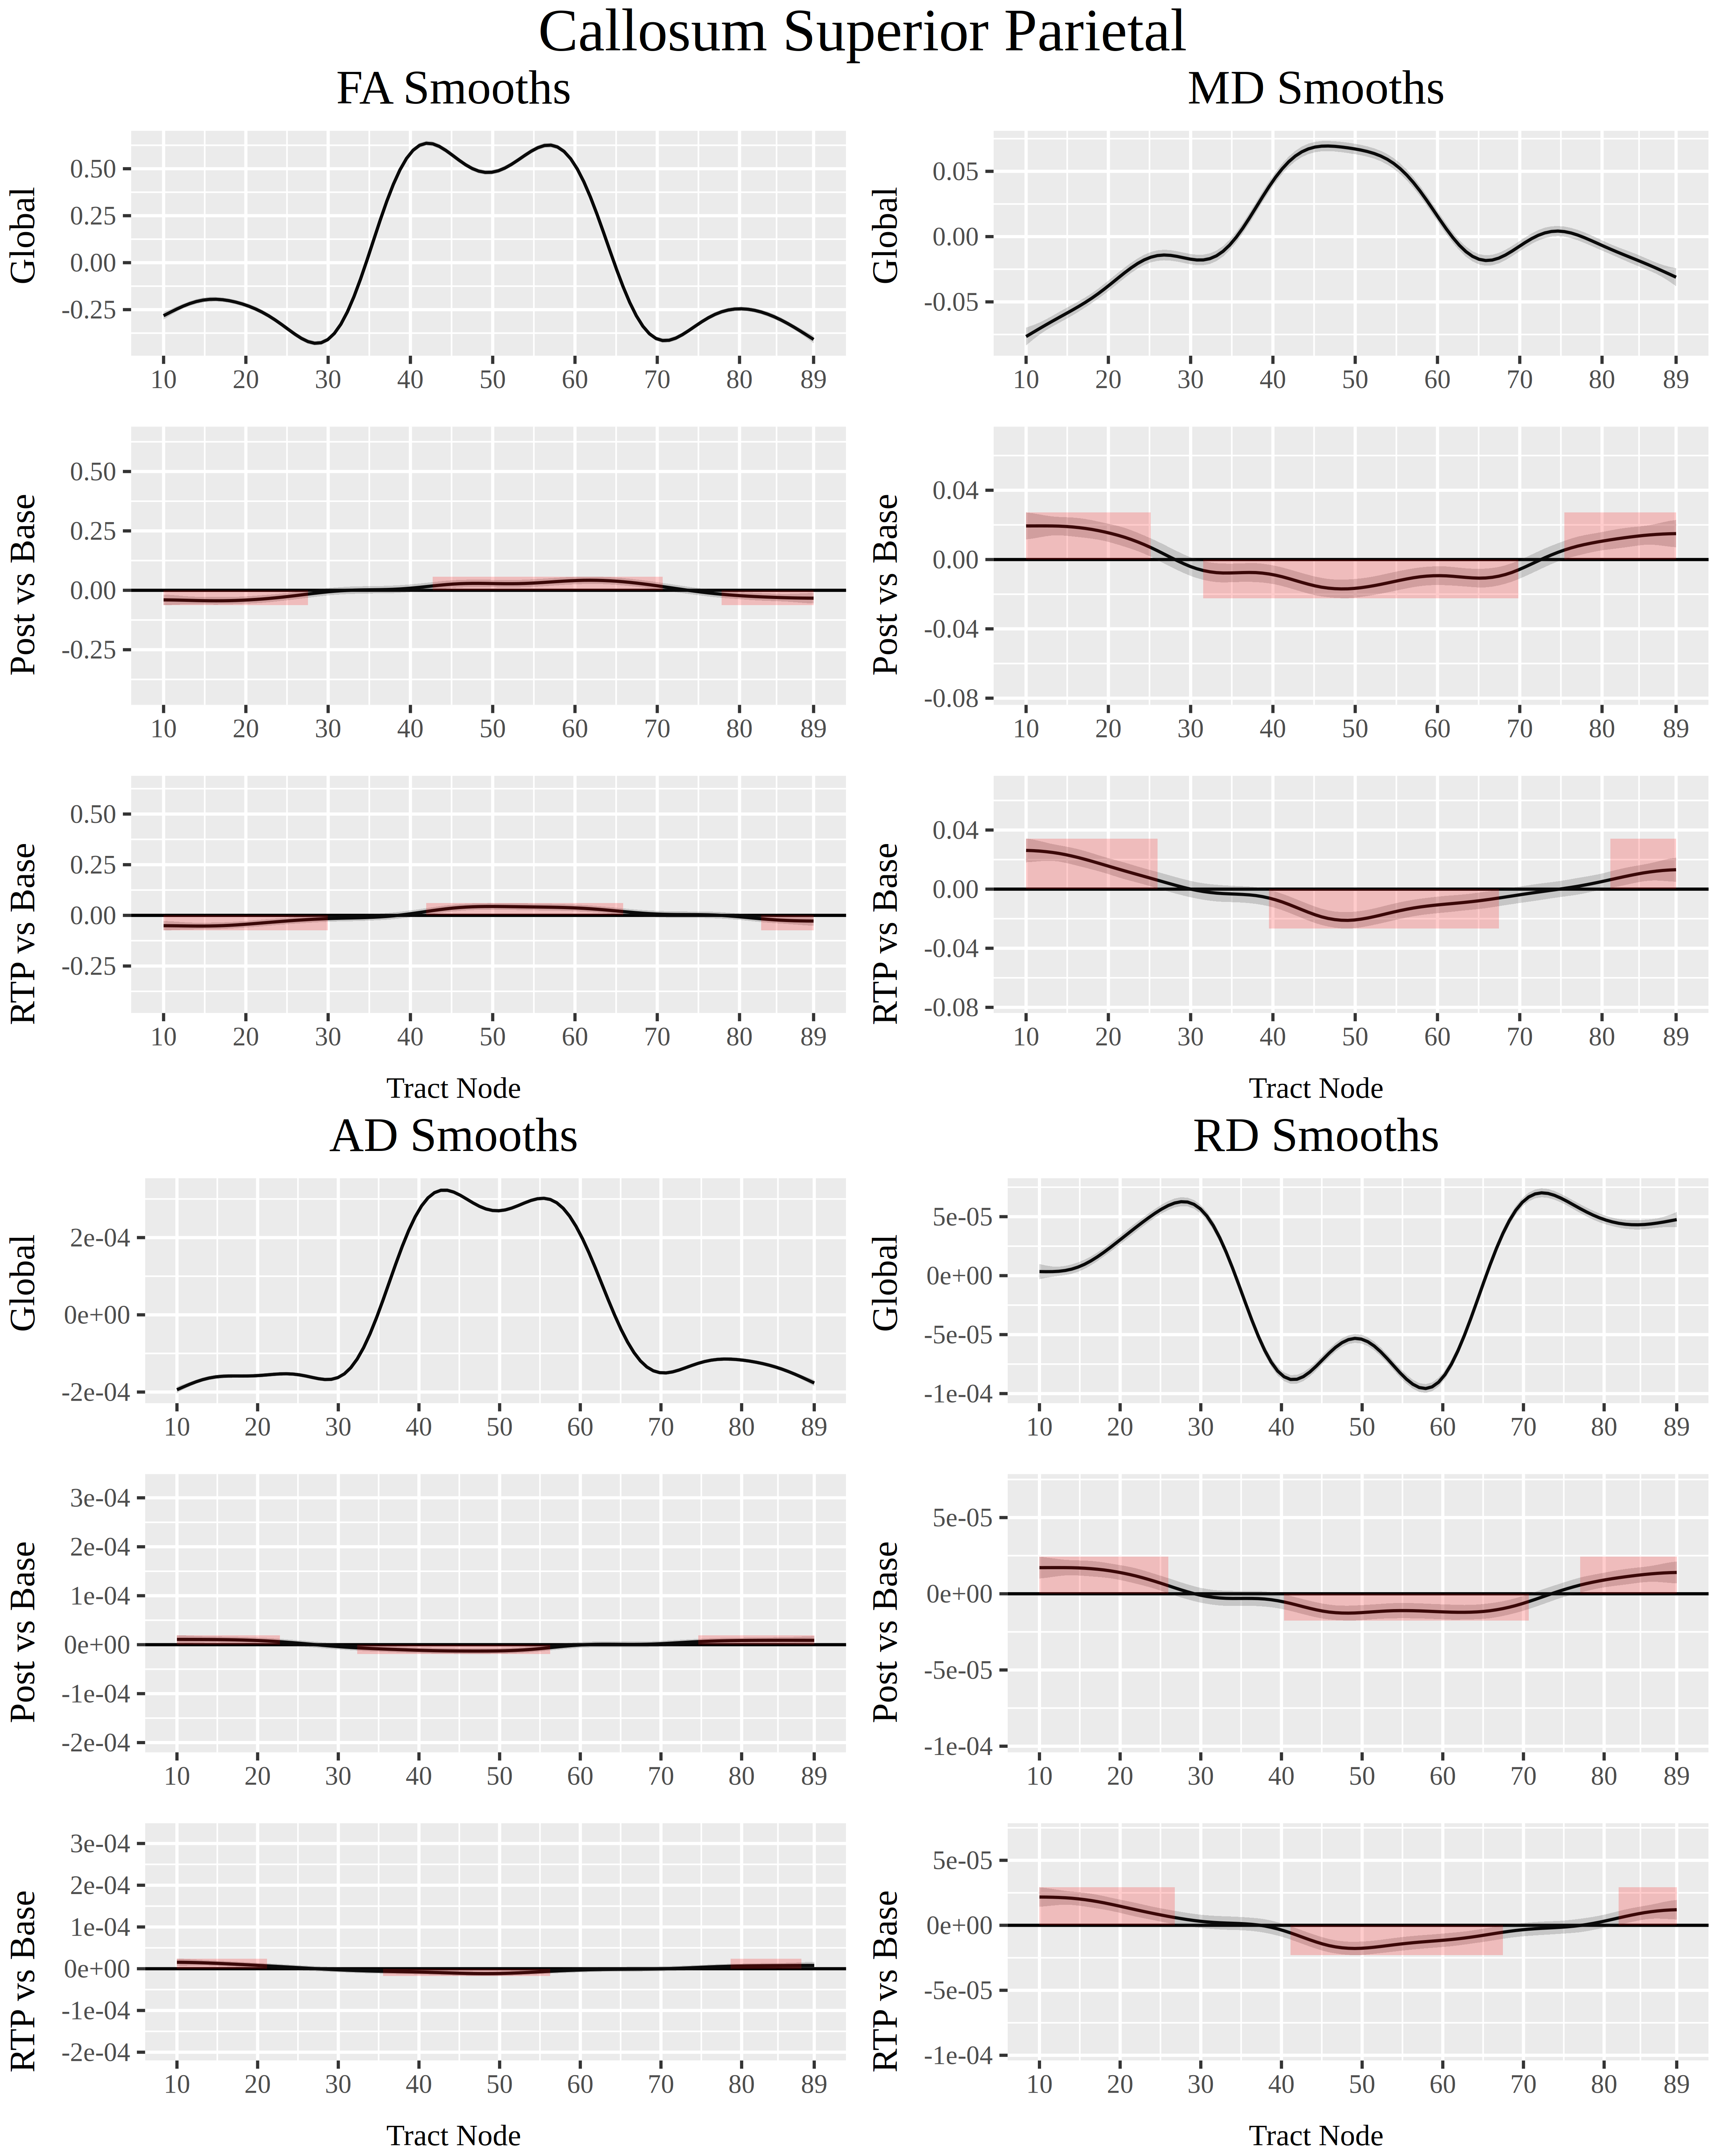
\includegraphics[width=.8\linewidth]{fit_LGIO_CCsp.png}}
	\caption{Longitudinal HGAM smooths modeling callosum superior parietal scalars as a function of node and visit. FA values are increased relative to Base at Post about node 50, with a corresponding decrease in RD at the same region. This pattern remains unchanged at RTP relative to Base.}
	\label{fig:lgio-gam-norecov}
\end{figure}

Further, increased FA corresponding with a decreased RD was identified about node 60 in the left corticospinal, node 65 in the right anterior thalamic, and node 45 in the right inferior fronto-occipital tracts (Supplemental Figure \ref{supp-fig:lgio-gam-norecov} a-c, respectively). AD values were also increased about node 40 in the right anterior thalamic tract at both Post and RTP vs. Base, and again this was counterbalanced by an increased RD in the same region, resulting in a lack of FA differences. As all four identified tracts demonstrated patterns consistent with cellular edema at Post which was unresolved at RTP, these data suggest that recovery from injury may yet be incomplete despite clearance to play.

All together, investigated FA changes in tracts identified by the longitudinal whole-brain model revealed complex injury sequelae that vary both anatomically and temporally. While evidence was generally found to support our second hypothesis, that tract FA changes would be the result of RD, but not AD, these were not always in the hypothesized direction (demyelination) and often indicated cellular or even cytotoxic edema. Further, we detected patterns of scalar change which indicate that athletes may not be fully recovered by the time they are cleared to return-to-play. Indeed, while we found evidence that concussion injury- and recovery-related scalar changes do occur, the majority of tract changes were either unresolved or in fact worse by the final visit. As athletes had an average 9$\pm$5.5 days between the Post and RTP visits in this study, it is possible that some individuals were cleared while still within the window of secondary injury cascades. Finally, we provided evidence that FA investigations may lack sensitivity in certain situations where both AD and RD have increased. While counterintuitive, such a change in scalars may result when there is both demyelination and glial scarring. When modeling such data, it is important to consider that injury sequelae, both within a tract and across time, may have non-linear properties, as we have demonstrated here, and that it is important to select tools with the appropriate sensitivity to model such properties.


\subsection{Tract FA Differences Relate to Changes in ImPACT Scores}
\label{ssec:res-dwi-imp}
In addition to modeling within-tract longitudinal scalar changes, HGAMs facilitate multimodal investigations through the use of tensor product interaction smooths. Clinical assessment metrics (or data from other modalities) can be included in higher dimensional models (R Code \ref{code:gam-lgio-intx}) to test whether such assessment metrics relate to concussion-related scalar change. We conducted exploratory analyses using the tracts identified above to determine whether FA changes related to ImPACT composite and total symptom scores. Specifically, we tested whether the tract FA-ImPACT interactions at Post and RTP differed from those at Base, where Post differences may link physiologic changes to clinical assessment and a lack of such differences at RTP potentially indicative recovery. These models tested the first part of our third hypothesis, that within-tract FA changes would correlate with clinical outcomes. Additionally, while tensor product interaction smooths can model non-linearities in the interaction terms, we specifically sought a linear FA-ImPACT interaction at a nodal region identified above, reasoning that a larger FA change at Post from Base would relate to worse clinical outcomes (Figure \ref{fig:intro-hyp}, right). Finally, we considered the node-FA-ImPACT interaction relevant for the study if the interaction term at RTP returned to near Base values.

Of the tracts tested, four were identified containing our expected interaction terms: the callosum superior frontal FA changes interacted with both visual memory and total symptoms, callosum superior parietal with total symptoms, and left corticospinal with reaction time (Figure \ref{fig:lgio-intx-imp}). Test statistics (Table \ref{tbl:lgio-intx-imp}, top) reveal that while controlling for the curvature of the tract and the main interaction effect, a significant differential interaction exists at Post relative to Base (ImPACT-Node:O.Post) that is also reduced at RTP (ImPACT-Node:O.RTP).

\begin{figure}[H]
	\captionsetup{labelformat=empty,oneside,margin={-75mm,0cm},captionskip=-103mm} % Use for splitting caption, align a-d with top left corner
	% \captionsetup[subfigure]{oneside,margin={-75mm,0cm},captionskip=-103mm} % Align a-d with top left corner
	\subfloat[]{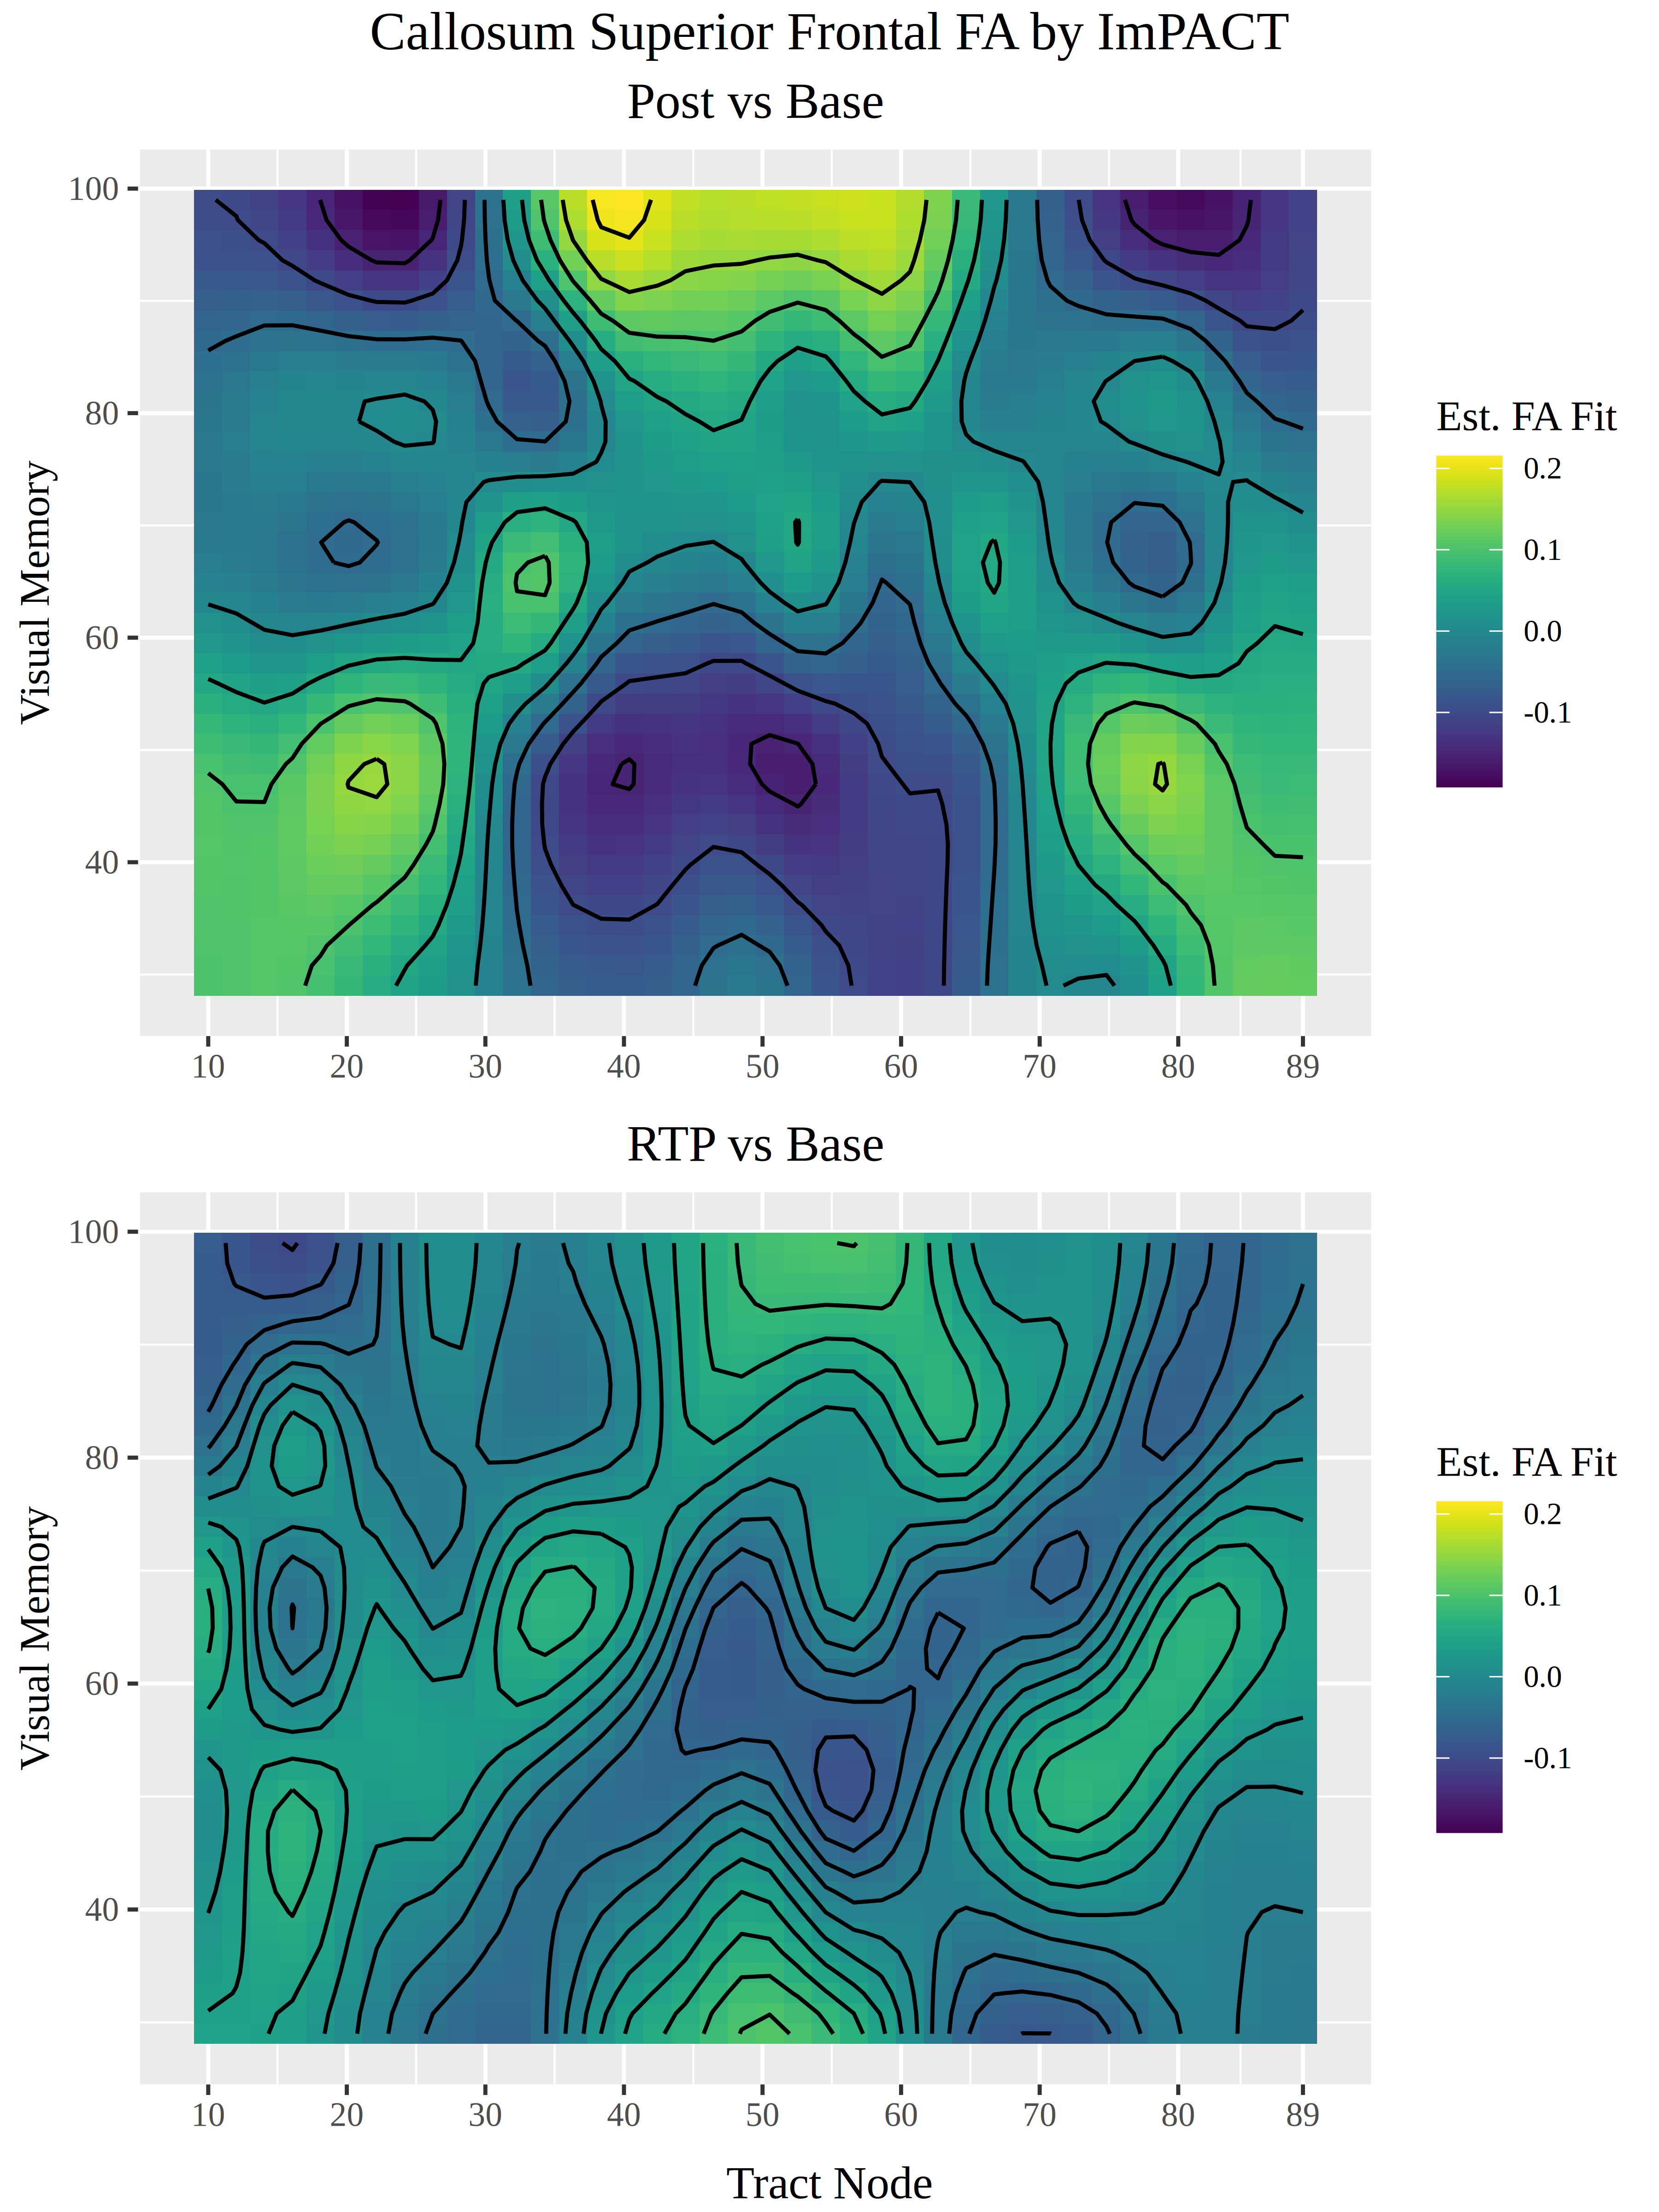
\includegraphics[width=3in]{fit_LGIO_intx_CCsf_mem_vis.png}}
	\subfloat[]{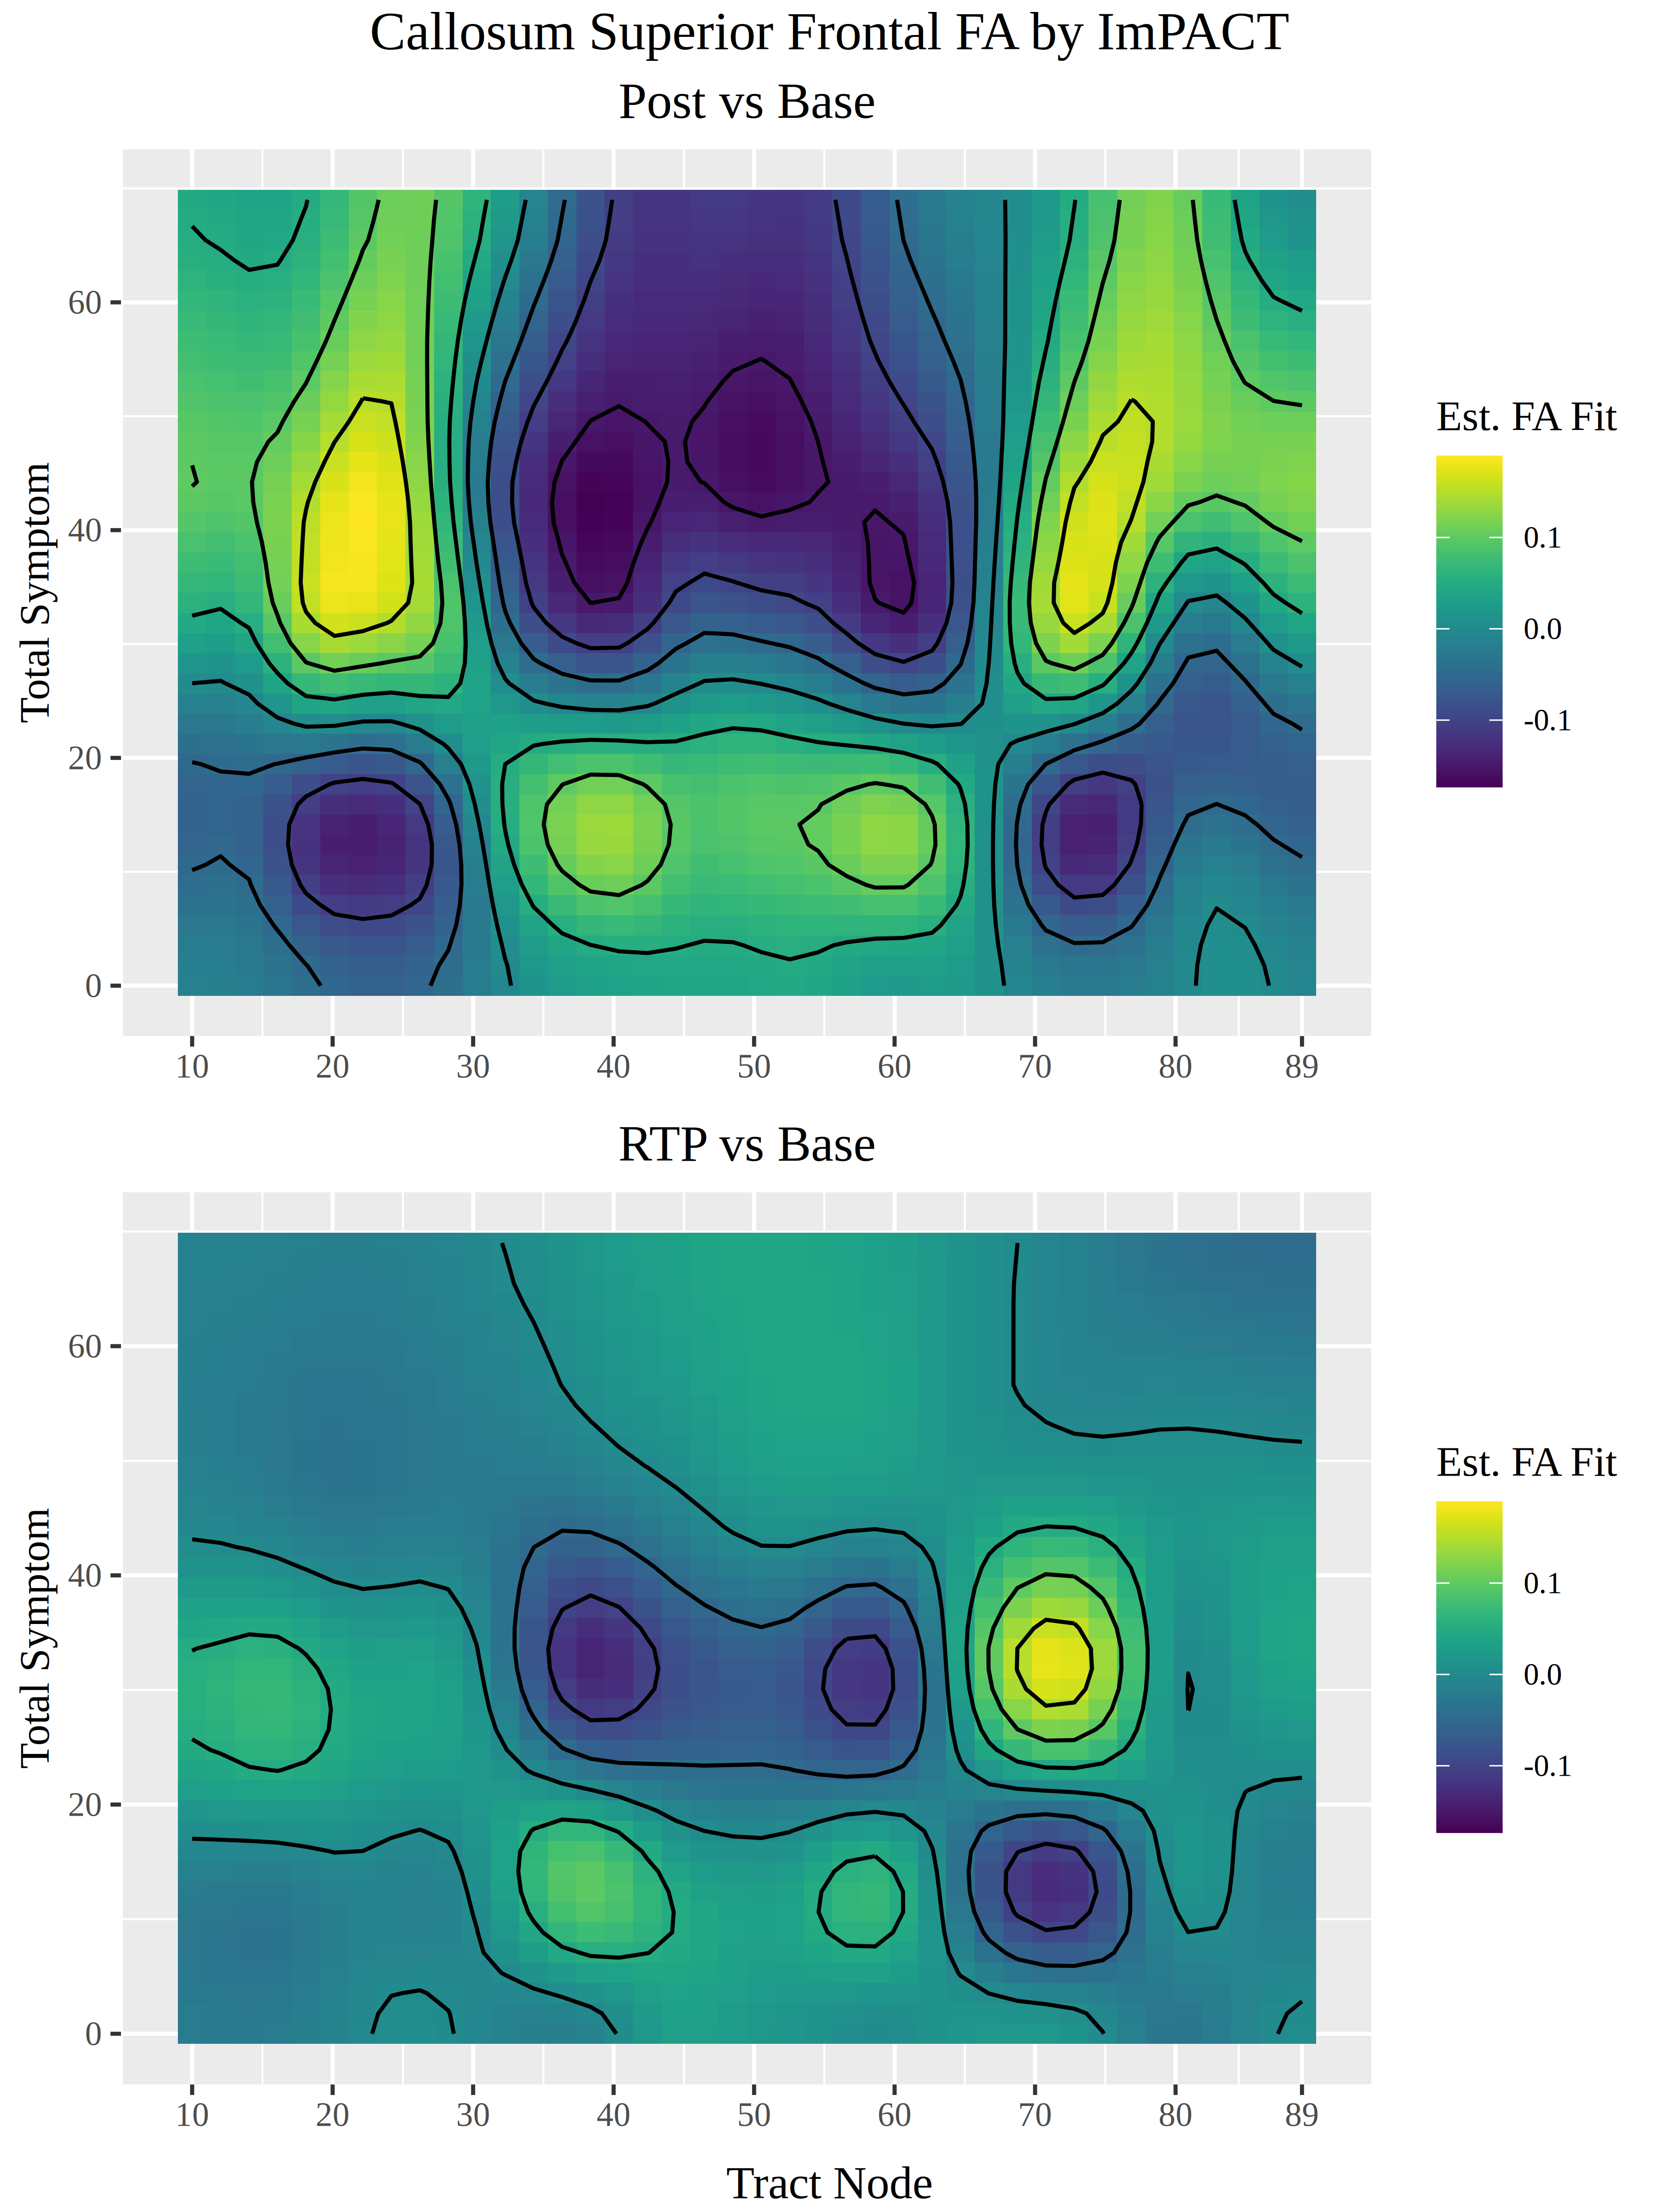
\includegraphics[width=3in]{fit_LGIO_intx_CCsf_tot_symp.png}}\\
	\subfloat[]{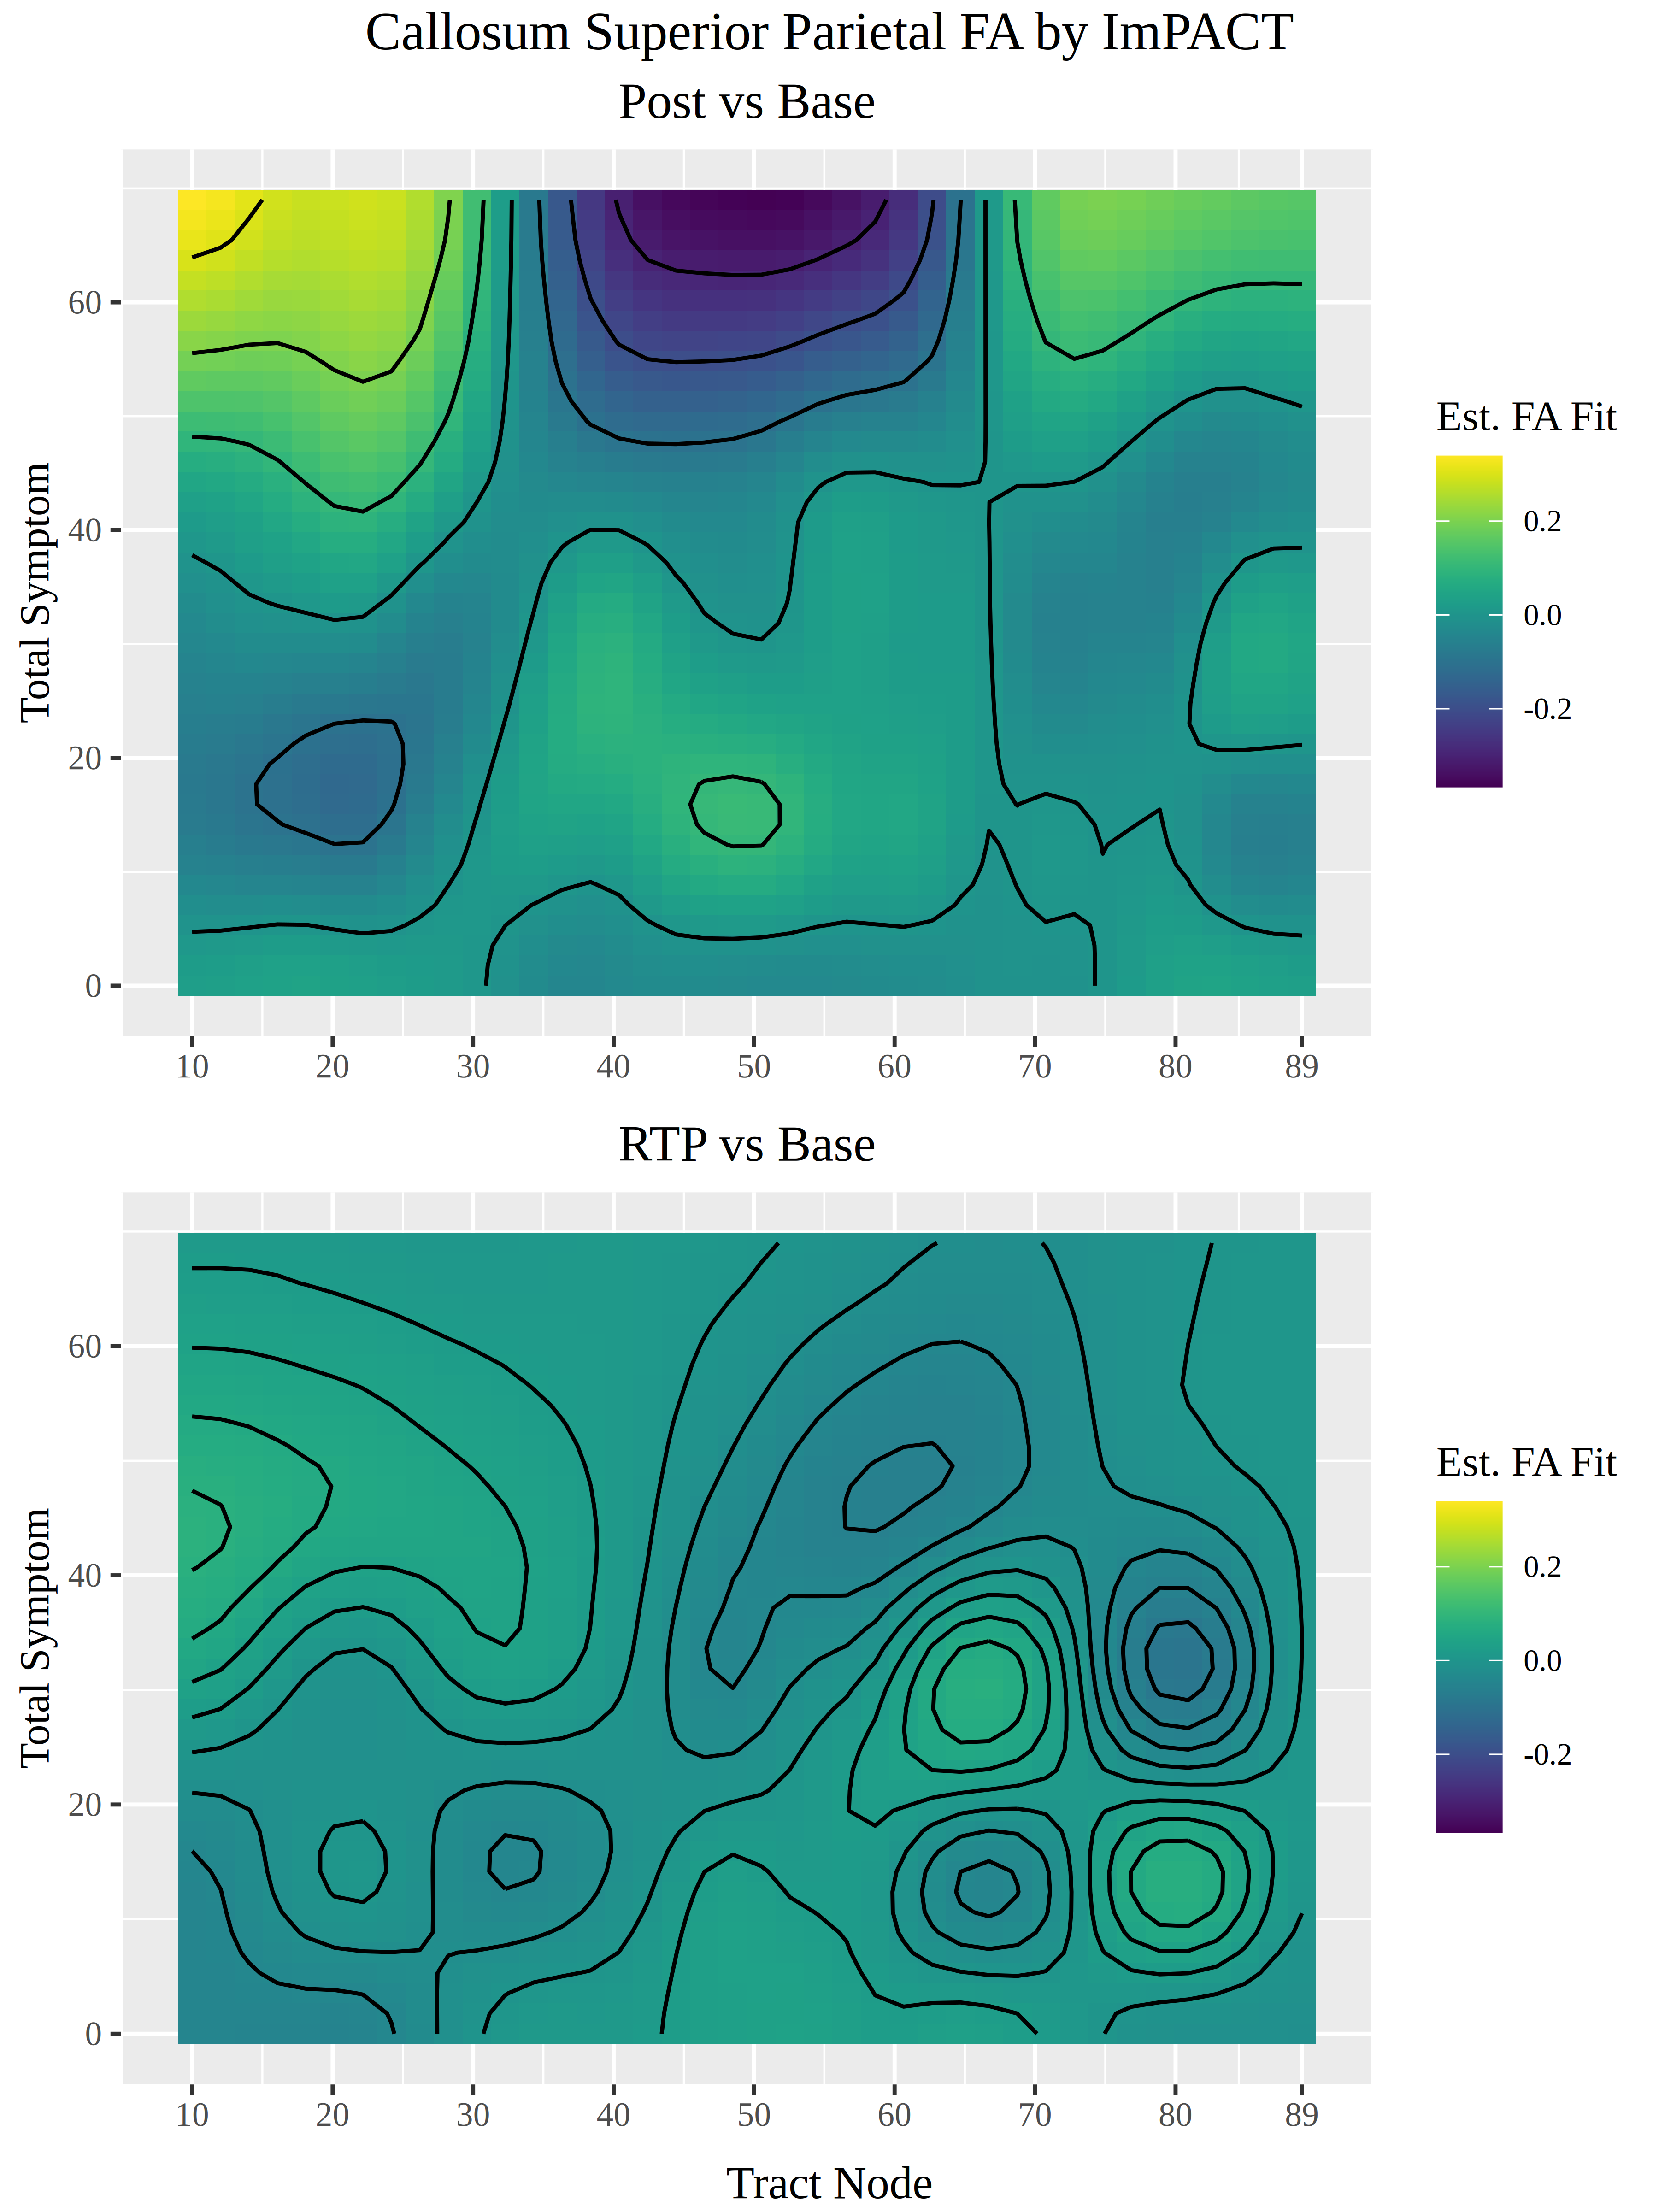
\includegraphics[width=3in]{fit_LGIO_intx_CCsp_tot_symp.png}}
	\subfloat[]{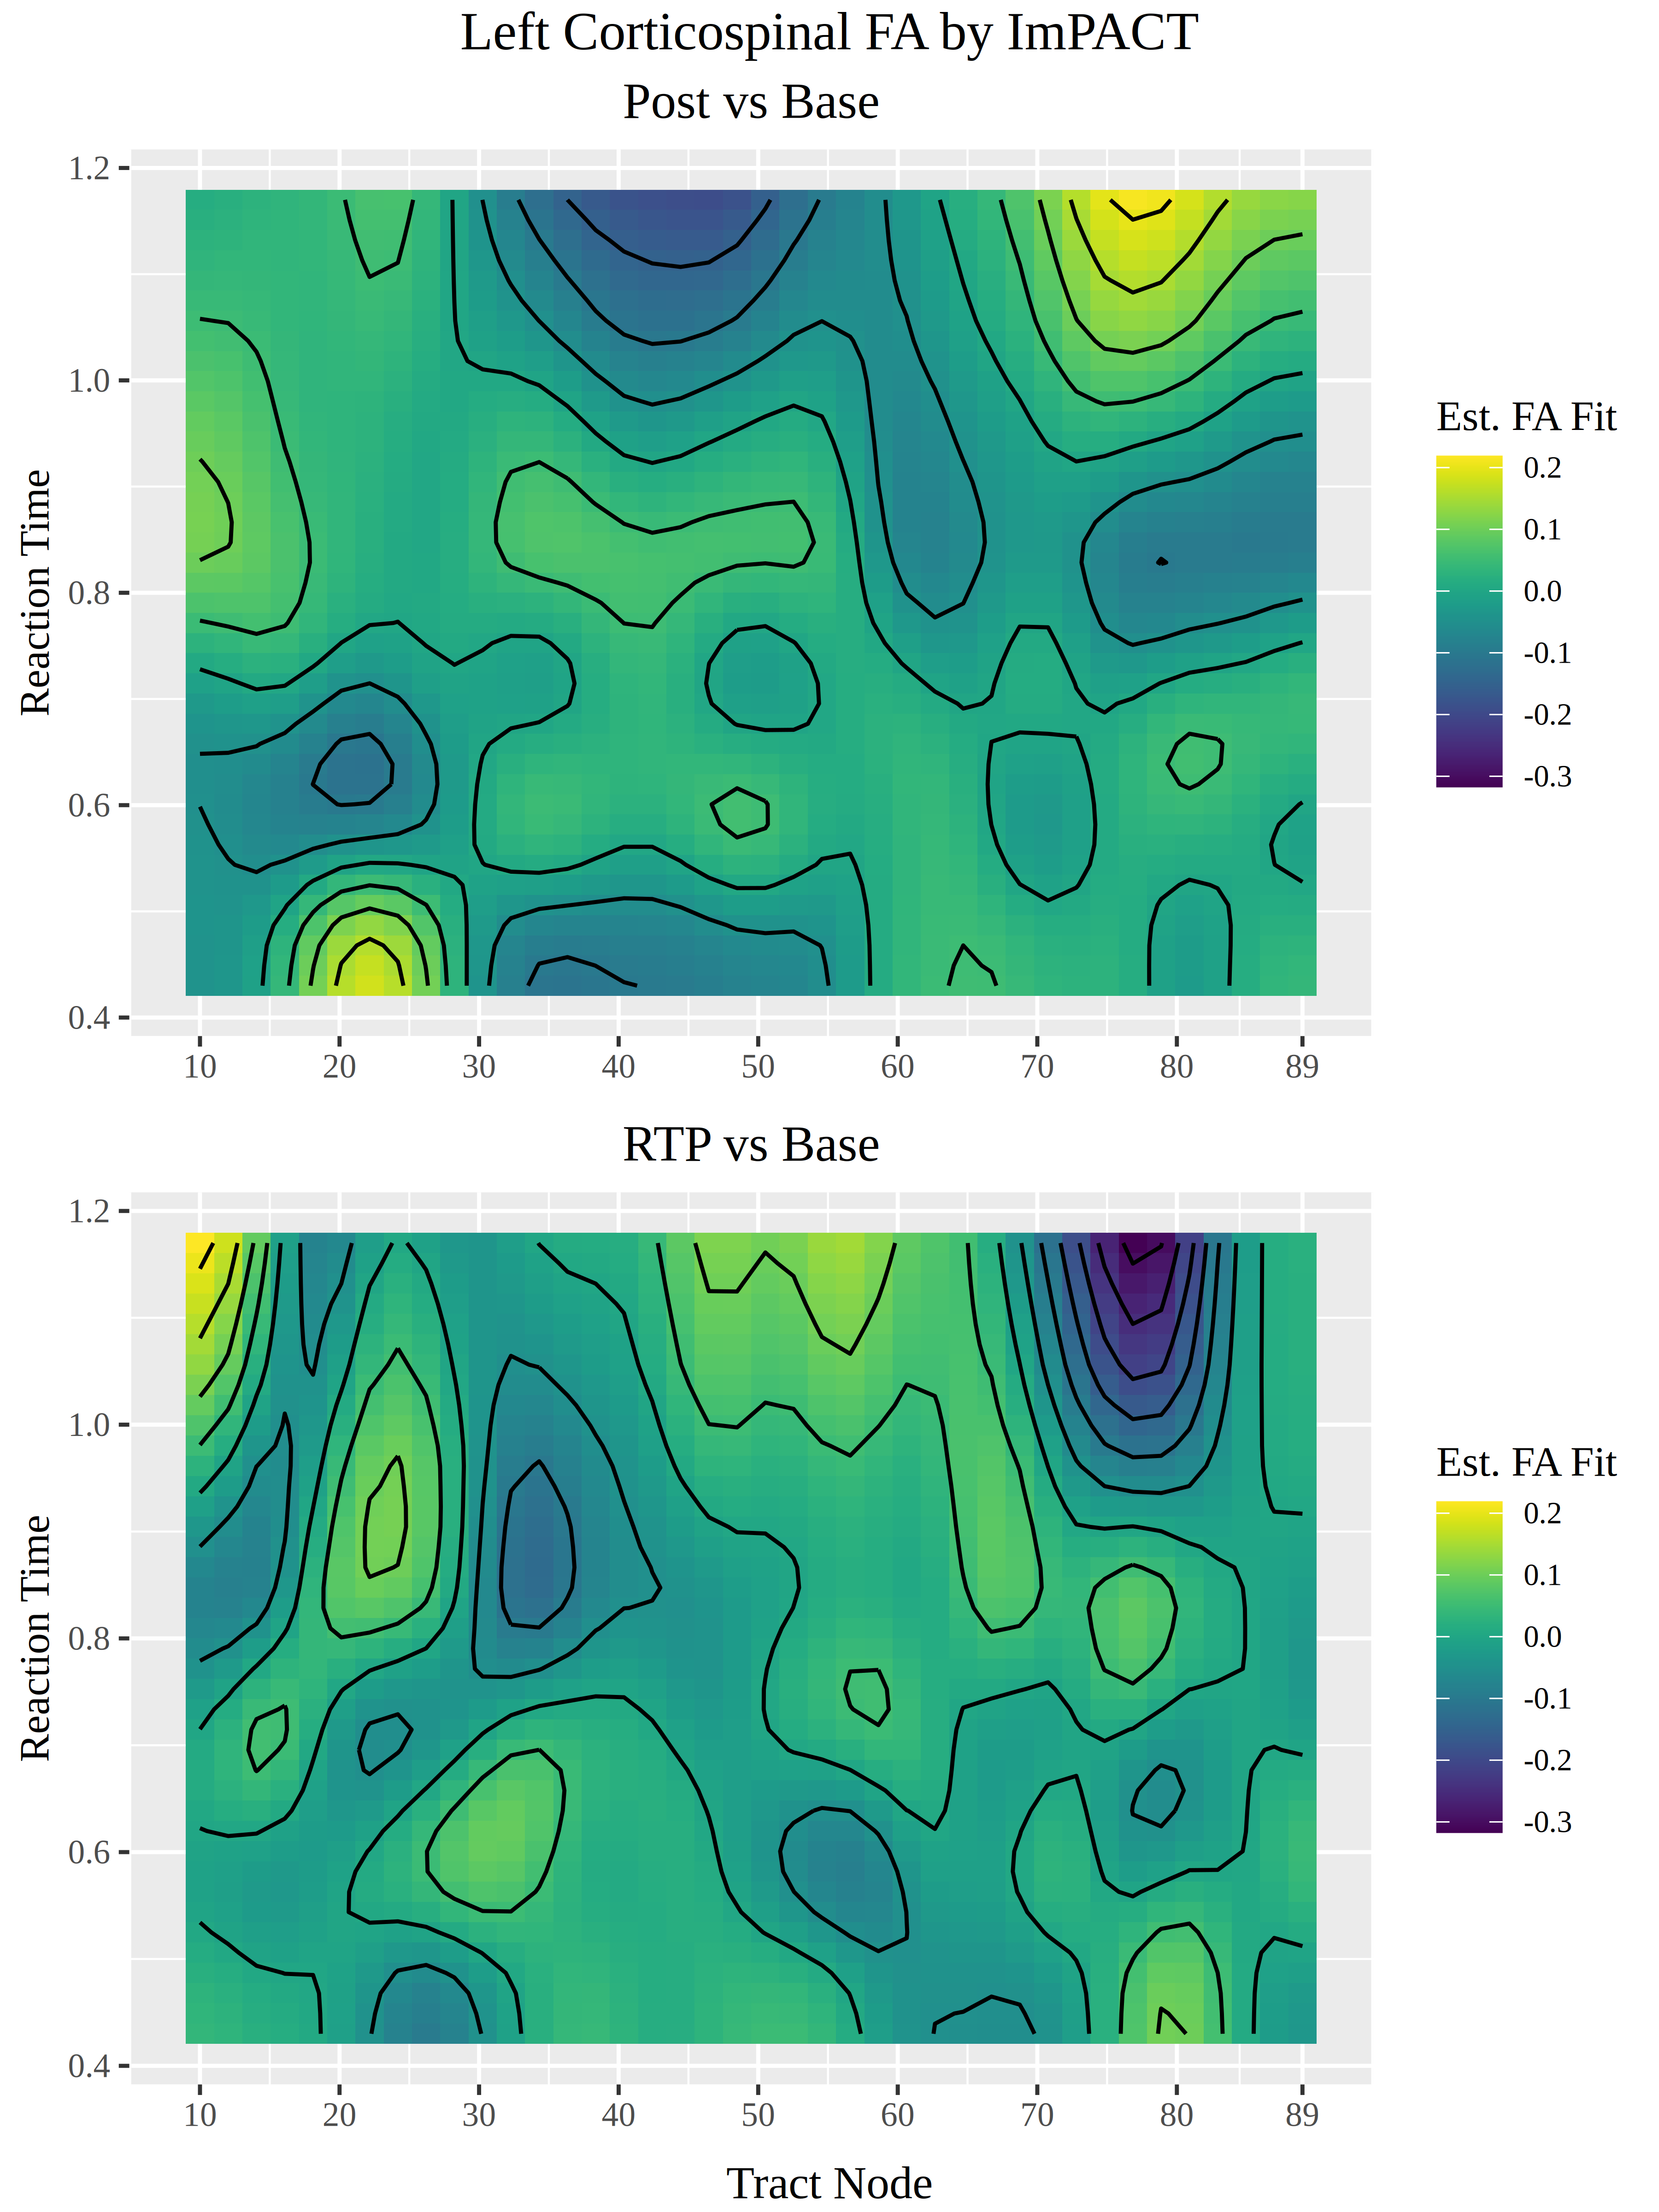
\includegraphics[width=3in]{fit_LGIO_intx_lCS_rx_time.png}}
	\caption{}
	% \captionsetup{} % reset caption specs
	% \caption{HGAM tensor product interaction difference smooths, comparing Post and RTP node-FA-ImPACT interactions terms with Base. A linear interaction is present at Post in each quadrant (top plots), indicated by a gradient (Z-axis) change along the Y-axis at a specific node (X-axis) region. This interaction is diminished or not found at RTP (bottom plots).}
	% \label{fig:lgio-intx-imp}
\end{figure}
\clearpage
\begin{figure}
	\captionsetup{labelformat=adja-page}
	\ContinuedFloat
	\caption{HGAM tensor product interaction difference smooths, comparing Post and RTP node-FA-ImPACT interactions terms with Base. A linear interaction is present at Post in each quadrant (top plots), indicated by a gradient (Z-axis) change along the Y-axis at a specific node (X-axis) region. This interaction is diminished or not found at RTP (bottom plots).}
	\label{fig:lgio-intx-imp}
\end{figure}

Figure \ref{fig:lgio-intx-imp} visualizes Post and RTP tract node-FA-ImPACT difference interactions as topological surfaces to facilitate reviewing the pattern and magnitude of the tensor product interaction effects. A somewhat linear differential interaction at Post is found for each tract, and this difference from Base largely resolves by RTP. For instance, an interaction exists in the callosum superior frontal tract about nodes 40-60 at Post (the same nodes previously identified; Supplemental Figure \ref{supp-fig:lgio-gam-recov}) where lower visual memory scores are associated with decreased FA values (Figure \ref{fig:lgio-intx-imp} a). At RTP, although a linear interaction is still somewhat present, the magnitude of the effect is diminished, aligning with both clinical and axonal recovery.

\begin{table}[H]
	\scriptsize
	% Please add the following required packages to your document preamble:
% \usepackage[table,xcdraw]{xcolor}
% Beamer presentation requires \usepackage{colortbl} instead of \usepackage[table,xcdraw]{xcolor}

\begin{tabular}{lllllllllllll}
 & \multicolumn{3}{c|}{CCsf: VisMem} & \multicolumn{3}{c|}{CCsf: TotSymp} & \multicolumn{3}{c|}{CCsp: TotSymp} & \multicolumn{3}{c}{lCS: RxTime} \\ \cline{2-13}
Smooth & \multicolumn{1}{c}{edf} & \multicolumn{1}{c}{F} & \multicolumn{1}{c|}{Sig} & \multicolumn{1}{c}{edf} & \multicolumn{1}{c}{F} & \multicolumn{1}{c|}{Sig} & \multicolumn{1}{c}{edf} & \multicolumn{1}{c}{F} & \multicolumn{1}{c|}{Sig} & \multicolumn{1}{c}{edf} & \multicolumn{1}{c}{F} & \multicolumn{1}{c}{Sig} \\ \hline
\multicolumn{1}{l|}{Node} & 13.95 & 775.40 & \multicolumn{1}{l|}{***} & 13.93 & 527.98 & \multicolumn{1}{l|}{***} & 13.92 & 2378.29 & \multicolumn{1}{l|}{***} & 13.63 & 1695.49 & *** \\
\rowcolor[HTML]{C0C0C0}
\multicolumn{1}{l|}{\cellcolor[HTML]{C0C0C0}ImP:Base} & 1.00 & 0.92 & \multicolumn{1}{l|}{\cellcolor[HTML]{C0C0C0}} & 1.00 & 1.25 & \multicolumn{1}{l|}{\cellcolor[HTML]{C0C0C0}} & 1.69 & 0.77 & \multicolumn{1}{l|}{\cellcolor[HTML]{C0C0C0}} & 1.00 & 0.20 &  \\
\multicolumn{1}{l|}{ImP:Post} & 1.00 & 3.64 & \multicolumn{1}{l|}{} & 1.00 & 3.08 & \multicolumn{1}{l|}{} & 2.77 & 1.87 & \multicolumn{1}{l|}{} & 1.01 & 0.05 &  \\
\rowcolor[HTML]{C0C0C0}
\multicolumn{1}{l|}{\cellcolor[HTML]{C0C0C0}ImP:RTP} & 1.00 & 0.17 & \multicolumn{1}{l|}{\cellcolor[HTML]{C0C0C0}} & 1.34 & 0.25 & \multicolumn{1}{l|}{\cellcolor[HTML]{C0C0C0}} & 1.35 & 0.31 & \multicolumn{1}{l|}{\cellcolor[HTML]{C0C0C0}} & 1.01 & 1.08 &  \\
\multicolumn{1}{l|}{ImP-Node} & 37.14 & 1.93 & \multicolumn{1}{l|}{***} & 37.56 & 2.83 & \multicolumn{1}{l|}{***} & 46.82 & 3.72 & \multicolumn{1}{l|}{***} & 39.33 & 2.56 & *** \\
\rowcolor[HTML]{C0C0C0}
\multicolumn{1}{l|}{\cellcolor[HTML]{C0C0C0}ImP-Node:O.Post} & 51.17 & 7.09 & \multicolumn{1}{l|}{\cellcolor[HTML]{C0C0C0}***} & 46.69 & 5.67 & \multicolumn{1}{l|}{\cellcolor[HTML]{C0C0C0}***} & 53.46 & 3.99 & \multicolumn{1}{l|}{\cellcolor[HTML]{C0C0C0}***} & 44.18 & 2.29 & *** \\
\multicolumn{1}{l|}{ImP-Node:O.RTP} & 36.16 & 1.83 & \multicolumn{1}{l|}{***} & 22.24 & 1.25 & \multicolumn{1}{l|}{***} & 20.16 & 1.12 & \multicolumn{1}{l|}{***} & 44.36 & 1.65 & *** \\ \hline
 &  &  &  &  &  &  &  &  &  &  &  &  \\
 & \multicolumn{3}{c|}{CCsp} & \multicolumn{3}{c|}{CCorb} & \multicolumn{3}{c|}{lCS} & \multicolumn{3}{c}{rUnc} \\ \cline{2-13}
Smooth & \multicolumn{1}{c}{edf} & \multicolumn{1}{c}{F} & \multicolumn{1}{c|}{Sig} & \multicolumn{1}{c}{edf} & \multicolumn{1}{c}{F} & \multicolumn{1}{c|}{Sig} & \multicolumn{1}{c}{edf} & \multicolumn{1}{c}{F} & \multicolumn{1}{c|}{Sig} & \multicolumn{1}{c}{edf} & \multicolumn{1}{c}{F} & \multicolumn{1}{c}{Sig} \\ \hline
\multicolumn{1}{l|}{Node} & 3.90 & 3.45 & \multicolumn{1}{l|}{**} & 7.174 & 18.794 & \multicolumn{1}{l|}{***} & 5.77 & 4.06 & \multicolumn{1}{l|}{***} & 1.80 & 0.47 &  \\
\rowcolor[HTML]{C0C0C0}
\multicolumn{1}{l|}{\cellcolor[HTML]{C0C0C0}Days} & 1.00 & 0.42 & \multicolumn{1}{l|}{\cellcolor[HTML]{C0C0C0}} & 1.334 & 6.188 & \multicolumn{1}{l|}{\cellcolor[HTML]{C0C0C0}*} & 1.00 & 3.68 & \multicolumn{1}{l|}{\cellcolor[HTML]{C0C0C0}} & 1.08 & 1.52 &  \\
\multicolumn{1}{l|}{Days-Node} & 32.55 & 1.15 & \multicolumn{1}{l|}{***} & 62.78 & 15.613 & \multicolumn{1}{l|}{***} & 37.10 & 2.04 & \multicolumn{1}{l|}{***} & 38.39 & 2.25 & ***
\end{tabular}

	\caption{Longitudinal tract interaction statistics. \textbf{Top}: Tract by ImPACT metric interaction. While significant non-flatness is detected for all ImPACT-Node interactions, note the reduction in effective degrees of freedom and F-stat between Post and RTP. VisMem = Visual Memory, TotSymp = Total Symptom, RxTime = Reaction Time. Node = global node, ImP:Base/Post/RTP = main effects of ImPACT metric for each group, ImP-Node = interaction term of node and ImPACT, ImP-Node:O.Post/RTP = Post/RTP group interaction as an ordered factor (relative to Base). \textbf{Bottom}: Interaction of select tracts and days between Post and RTP. edf = effective degrees of freedom, F = F-statistic, Sig = significance. *** = p$<$.001, ** = p$<$.01, * = p$<$.05. See Figure \ref{fig:ldi-gam} for tract names.}
	\label{tbl:lgio-intx-imp}
\end{table}

Likewise, total symptoms are related to decreased FA values about callosum superior frontal in the same nodal region (Figure \ref{fig:lgio-intx-imp} b) and also in the callosum superior parietal (Figure \ref{fig:lgio-intx-imp} c, about node 50). Finally, reaction times associated with changes to left corticospinal FA values; at Post, the slowest reaction times corresponded to the largest FA values about node 75. This pattern which was reversed at RTP, likely due to sparsity in slow reaction times during this visit (Figure \ref{fig:imp-gam}, bottom right). In each case of these cases, the node-FA-ImPACT interaction was reduced at RTP, indicated by the `flatter' interaction difference surface, fewer effective degrees of freedom, and lower F-statistics (Table \ref{tbl:lgio-intx-imp}, top).


\subsection{Tract FA Differences Relate to Recovery Time}
\label{ssec:res-dwi-time}
We originally hypothesized that changes in FA values would relate recovery time, reasoning that more significant injuries i.e. larger deflections from baseline would necessitate a longer recovery period. To test this, we utilized tensor product interaction smooths to determine whether RTP vs. Post $\Delta$FA values related to the number of days between Post and RTP. From the tracts in which we previously detected concussion-related changes, four demonstrated node-$\Delta$FA-time interactions that aligned with predictions: the left corticospinal, right uncinate, callosum superior parietal, and callosum orbital (Table \ref{tbl:lgio-intx-imp}, bottom; Figure \ref{fig:di-time}). Within these tracts, two interaction patterns were detected.

\begin{figure}[H]
	\captionsetup[subfigure]{oneside,margin={-75mm,0cm},captionskip=-53mm} % Align a-d with top left corner
	\subfloat[]{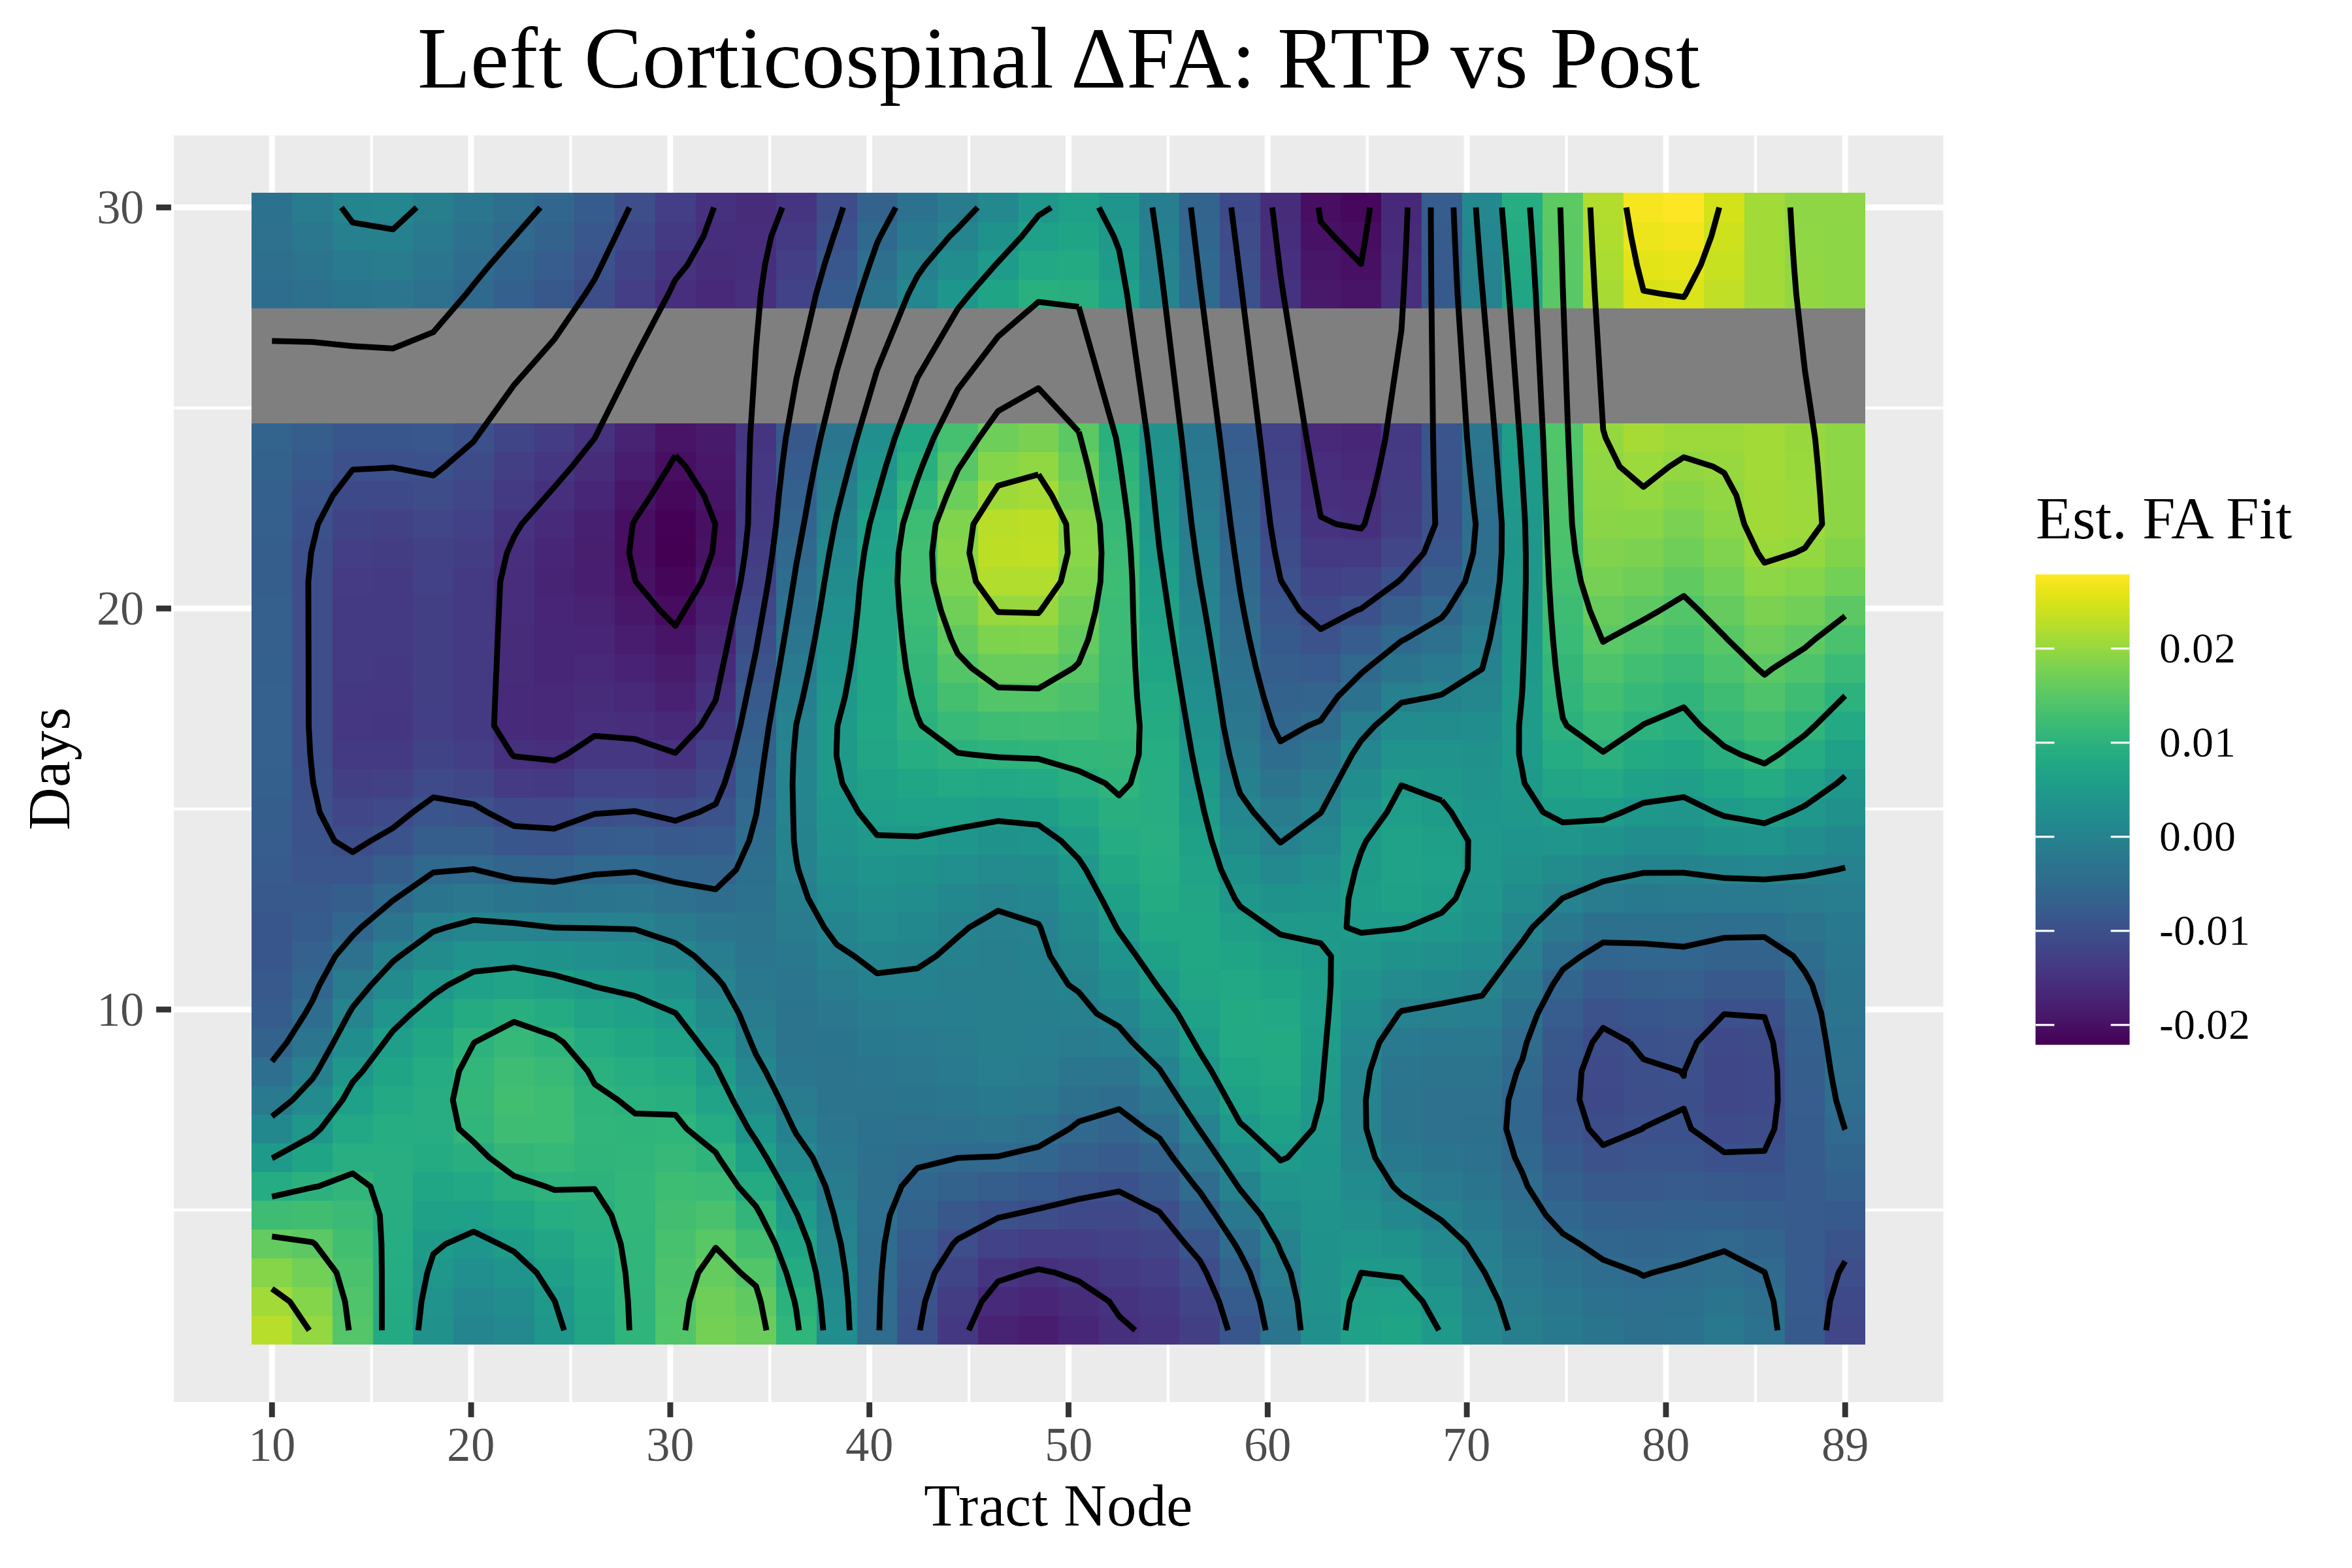
\includegraphics[width=3in]{fit_DI_time_lCS_fa.png}}
	\subfloat[]{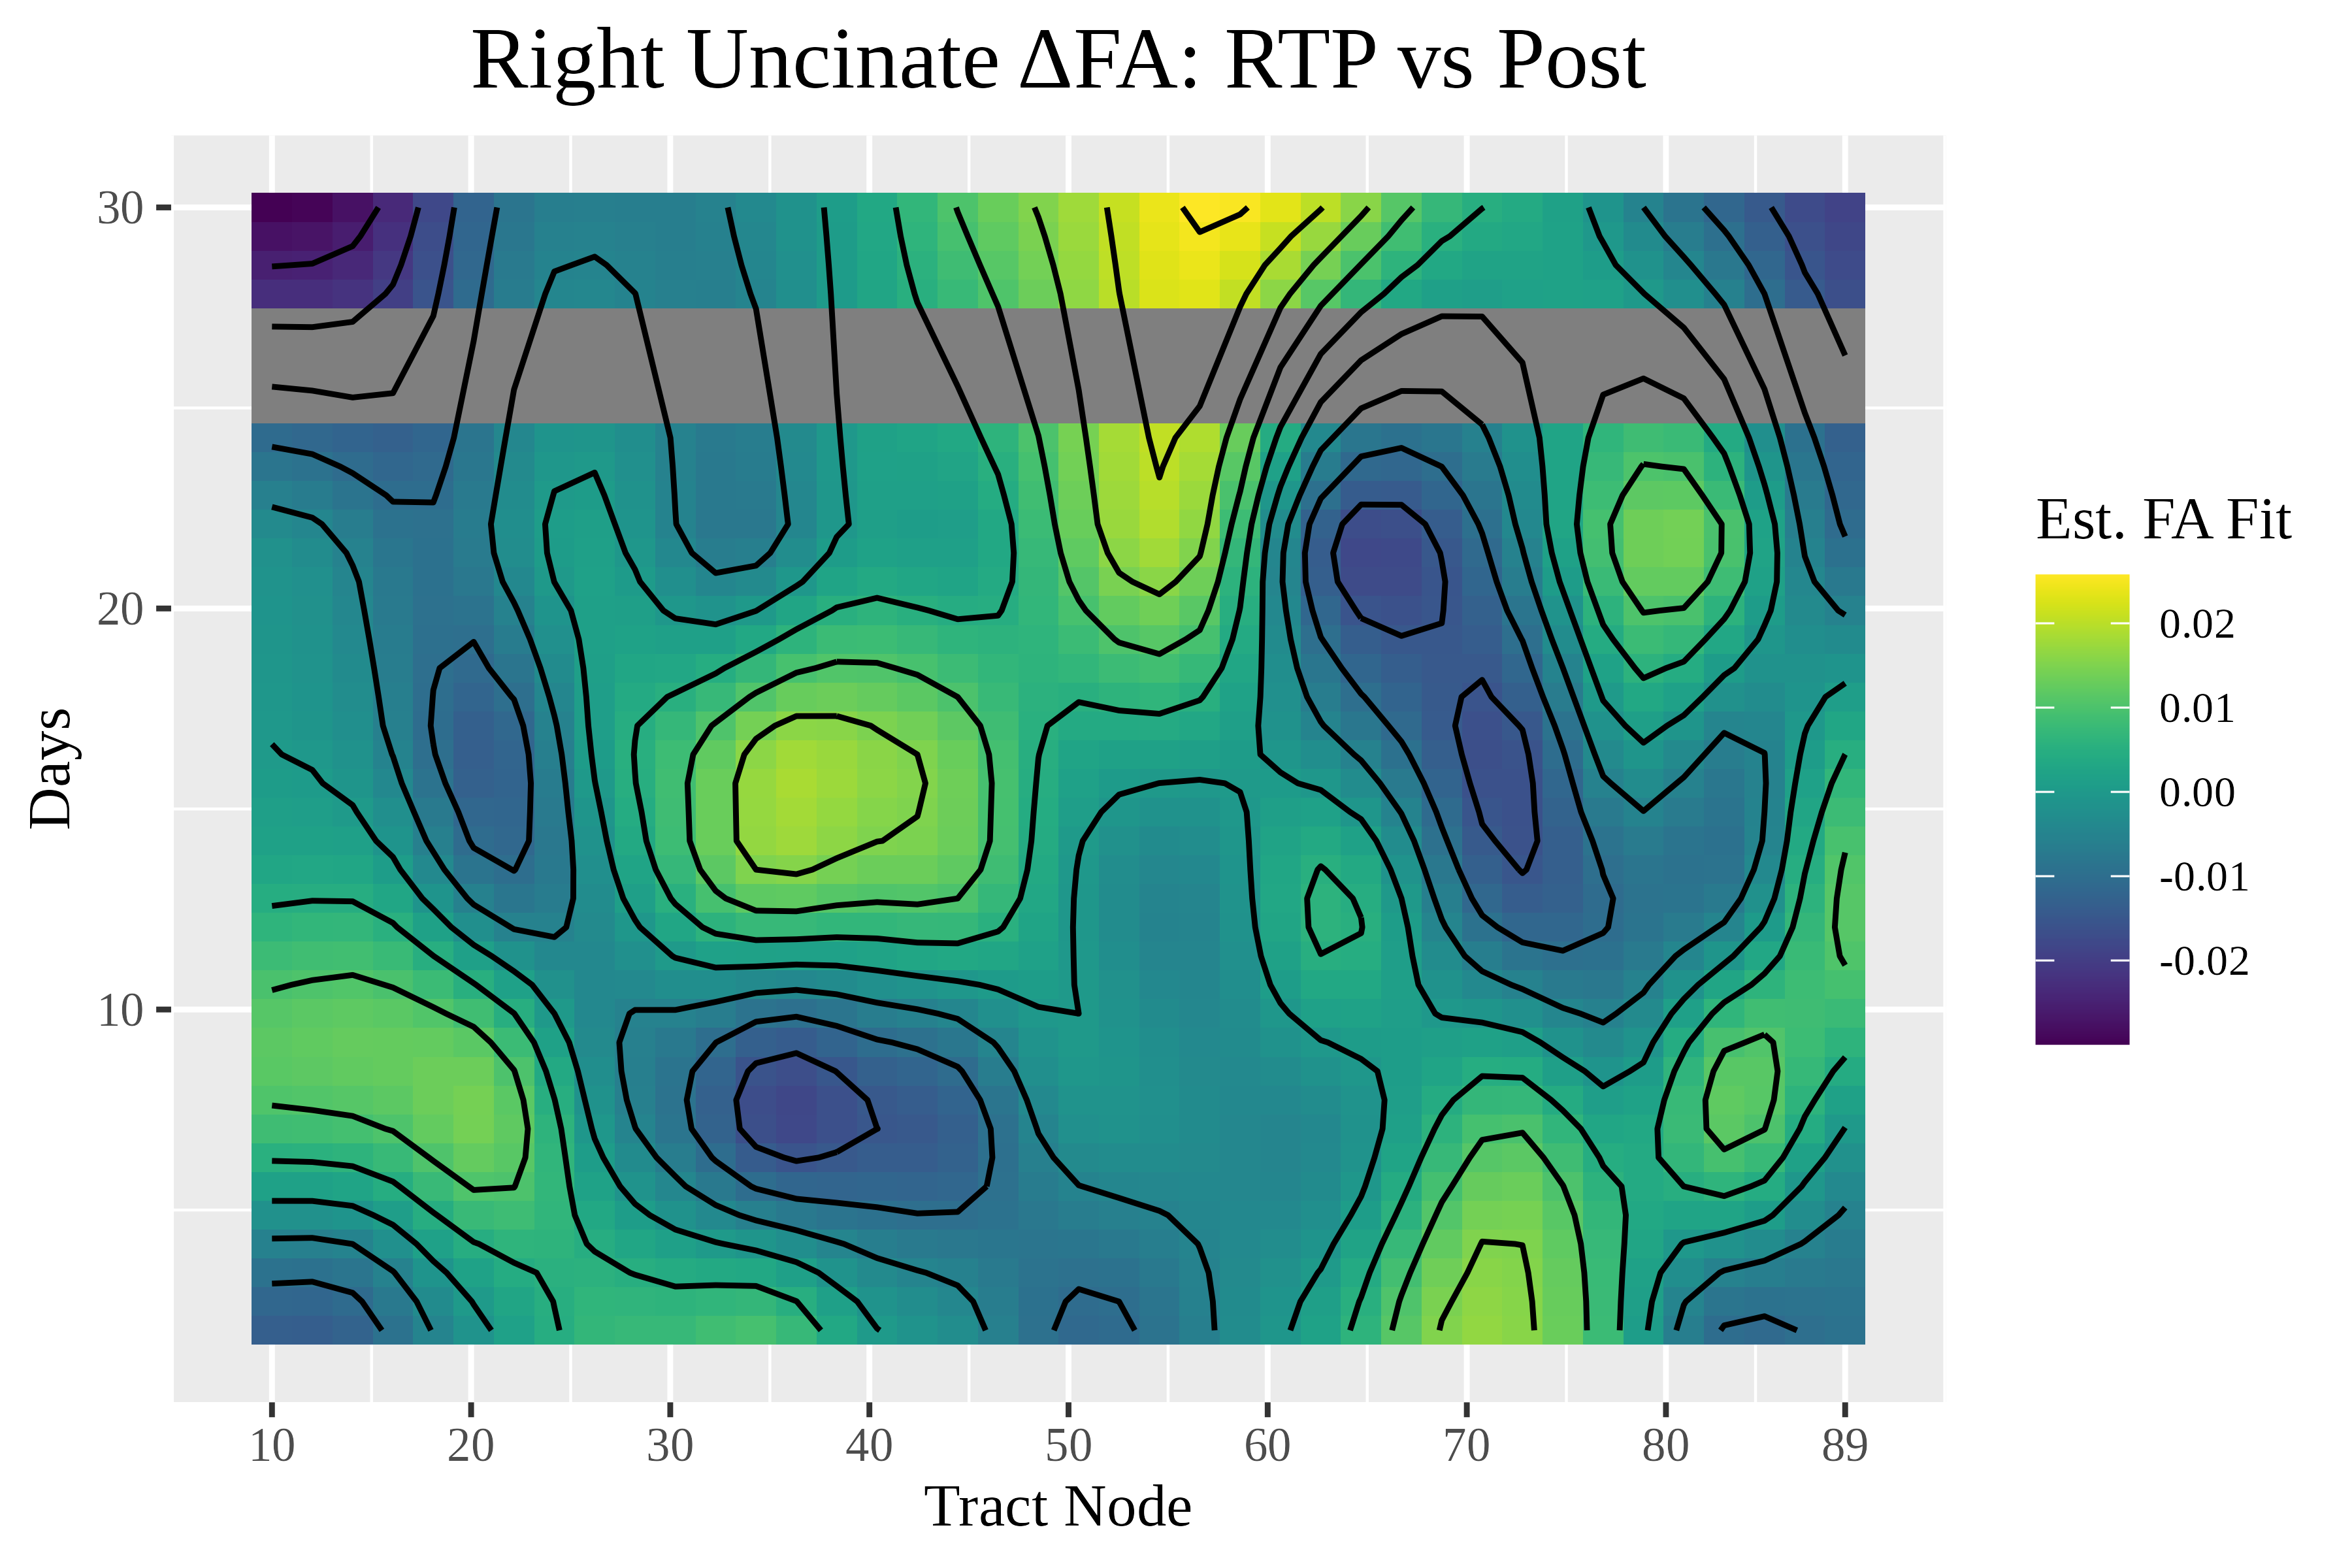
\includegraphics[width=3in]{fit_DI_time_rUnc_fa.png}}\\
	\subfloat[]{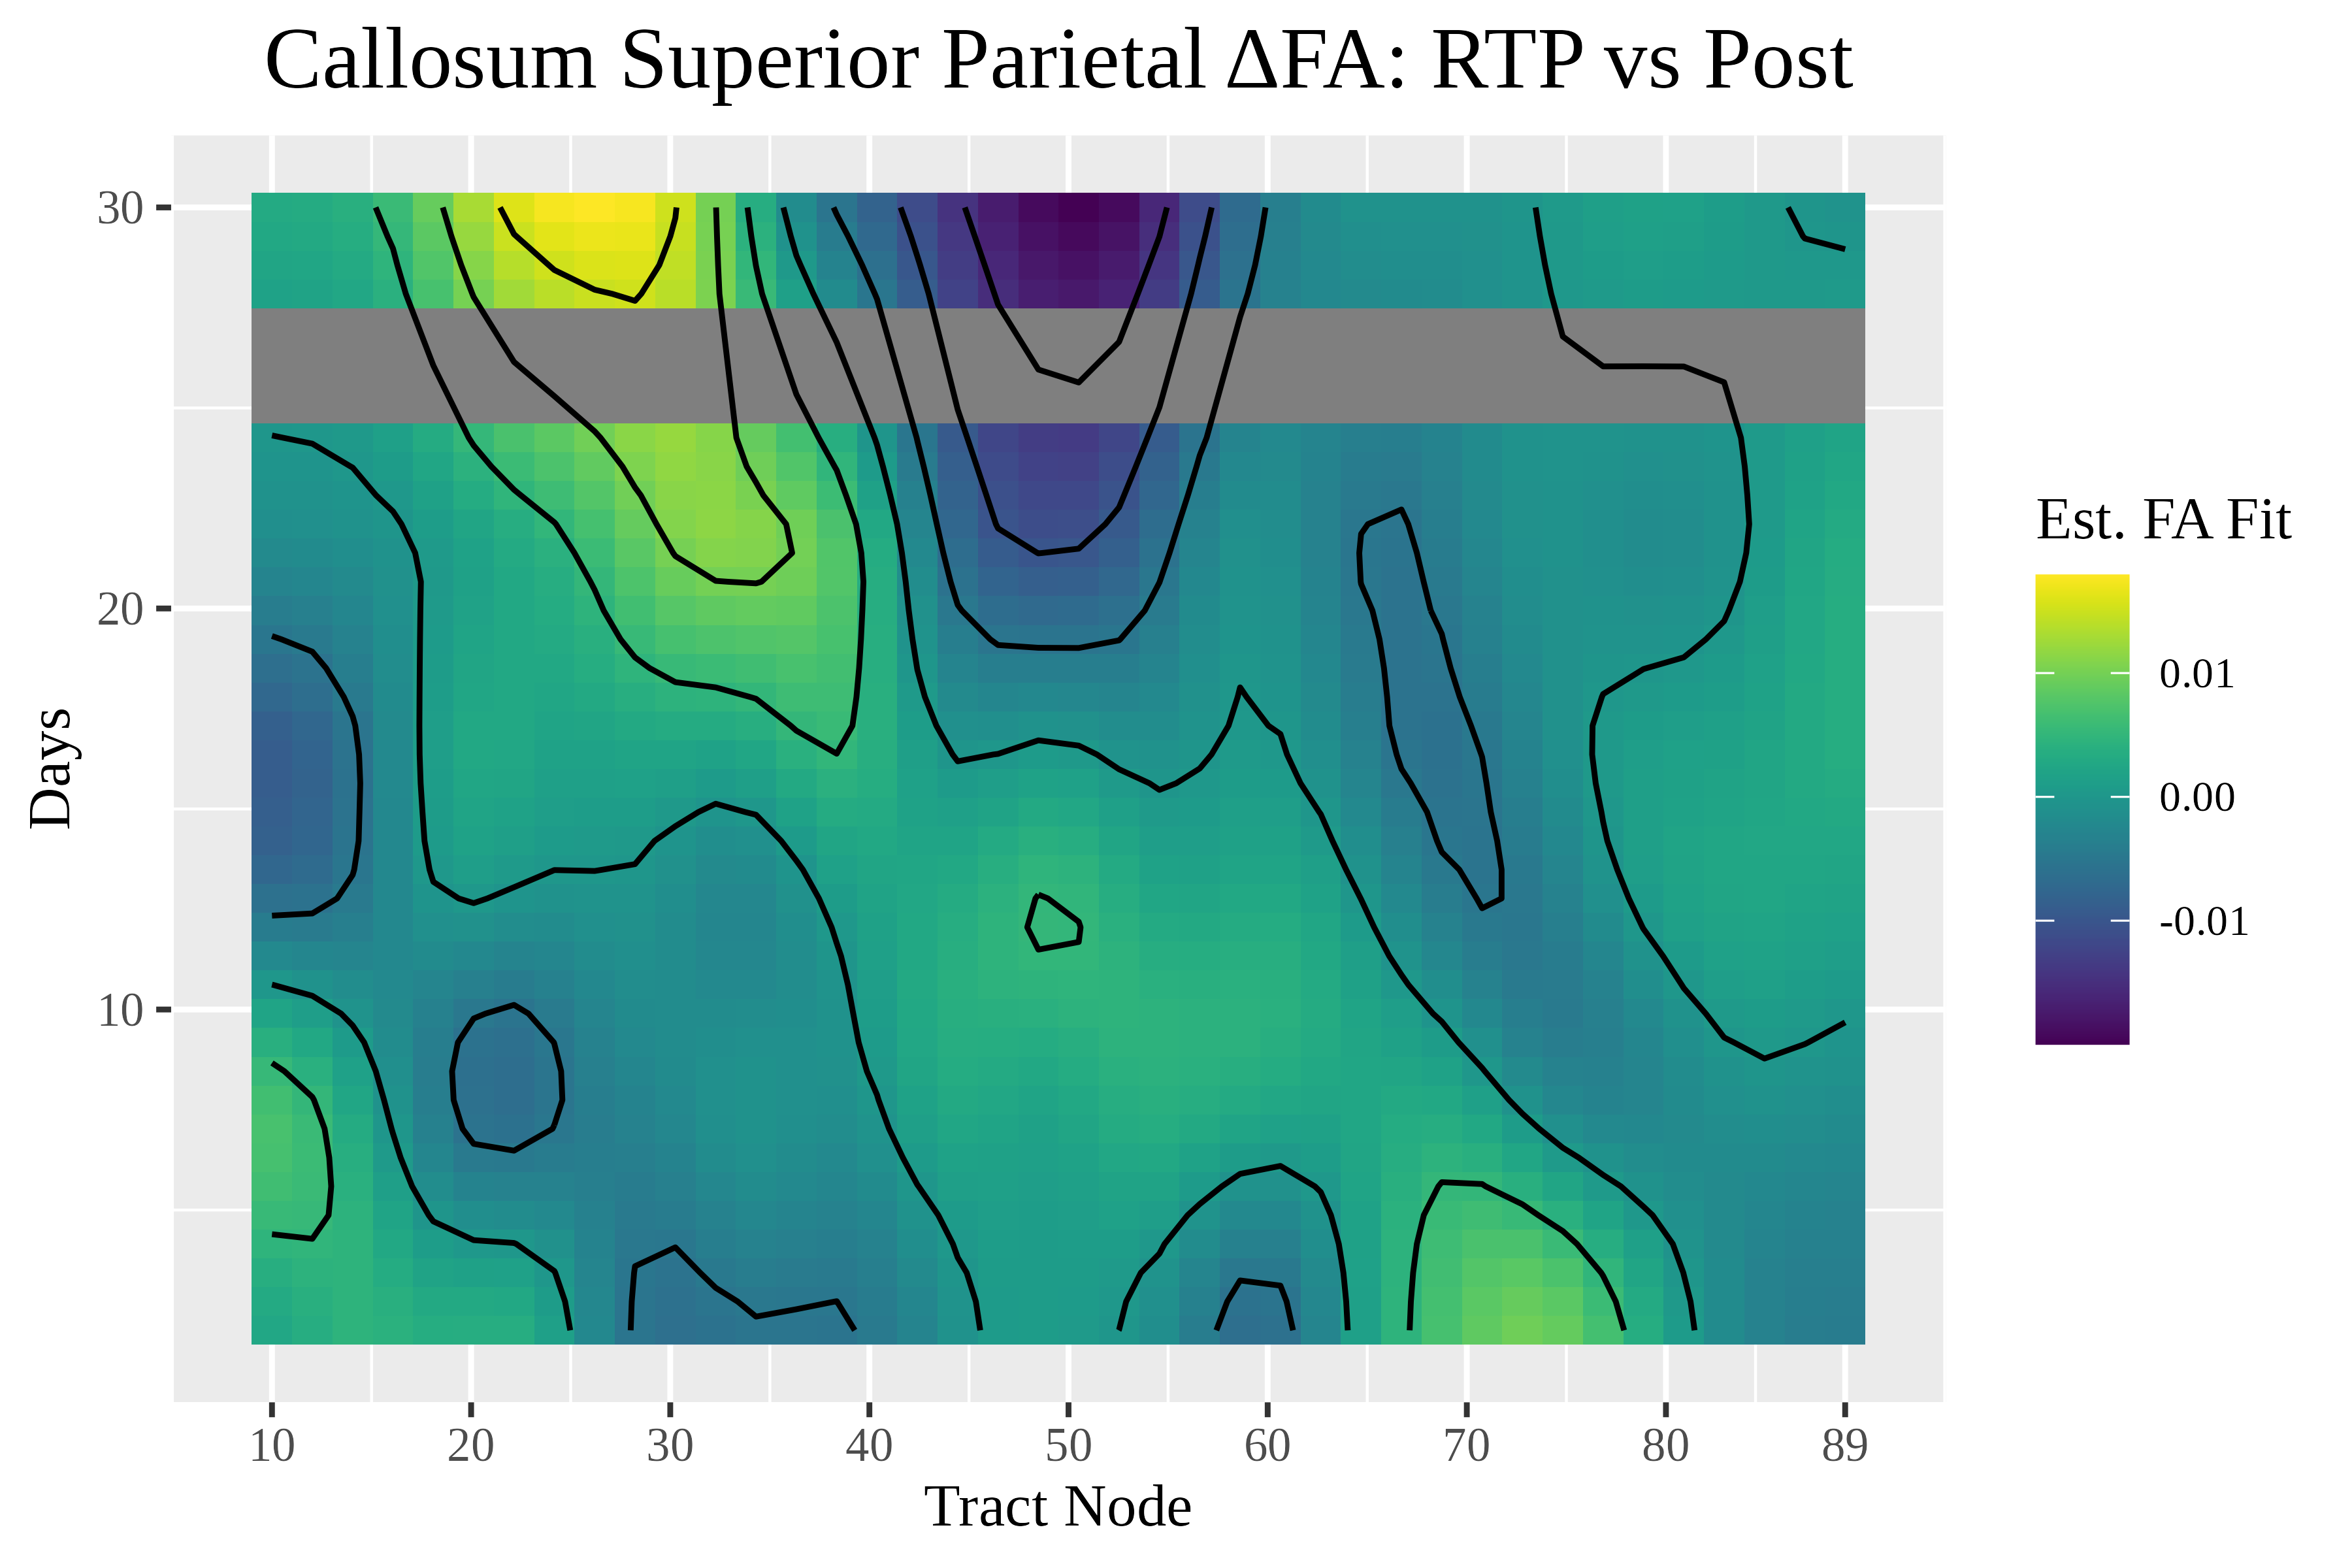
\includegraphics[width=3in]{fit_DI_time_CCsp_fa.png}}
	\subfloat[]{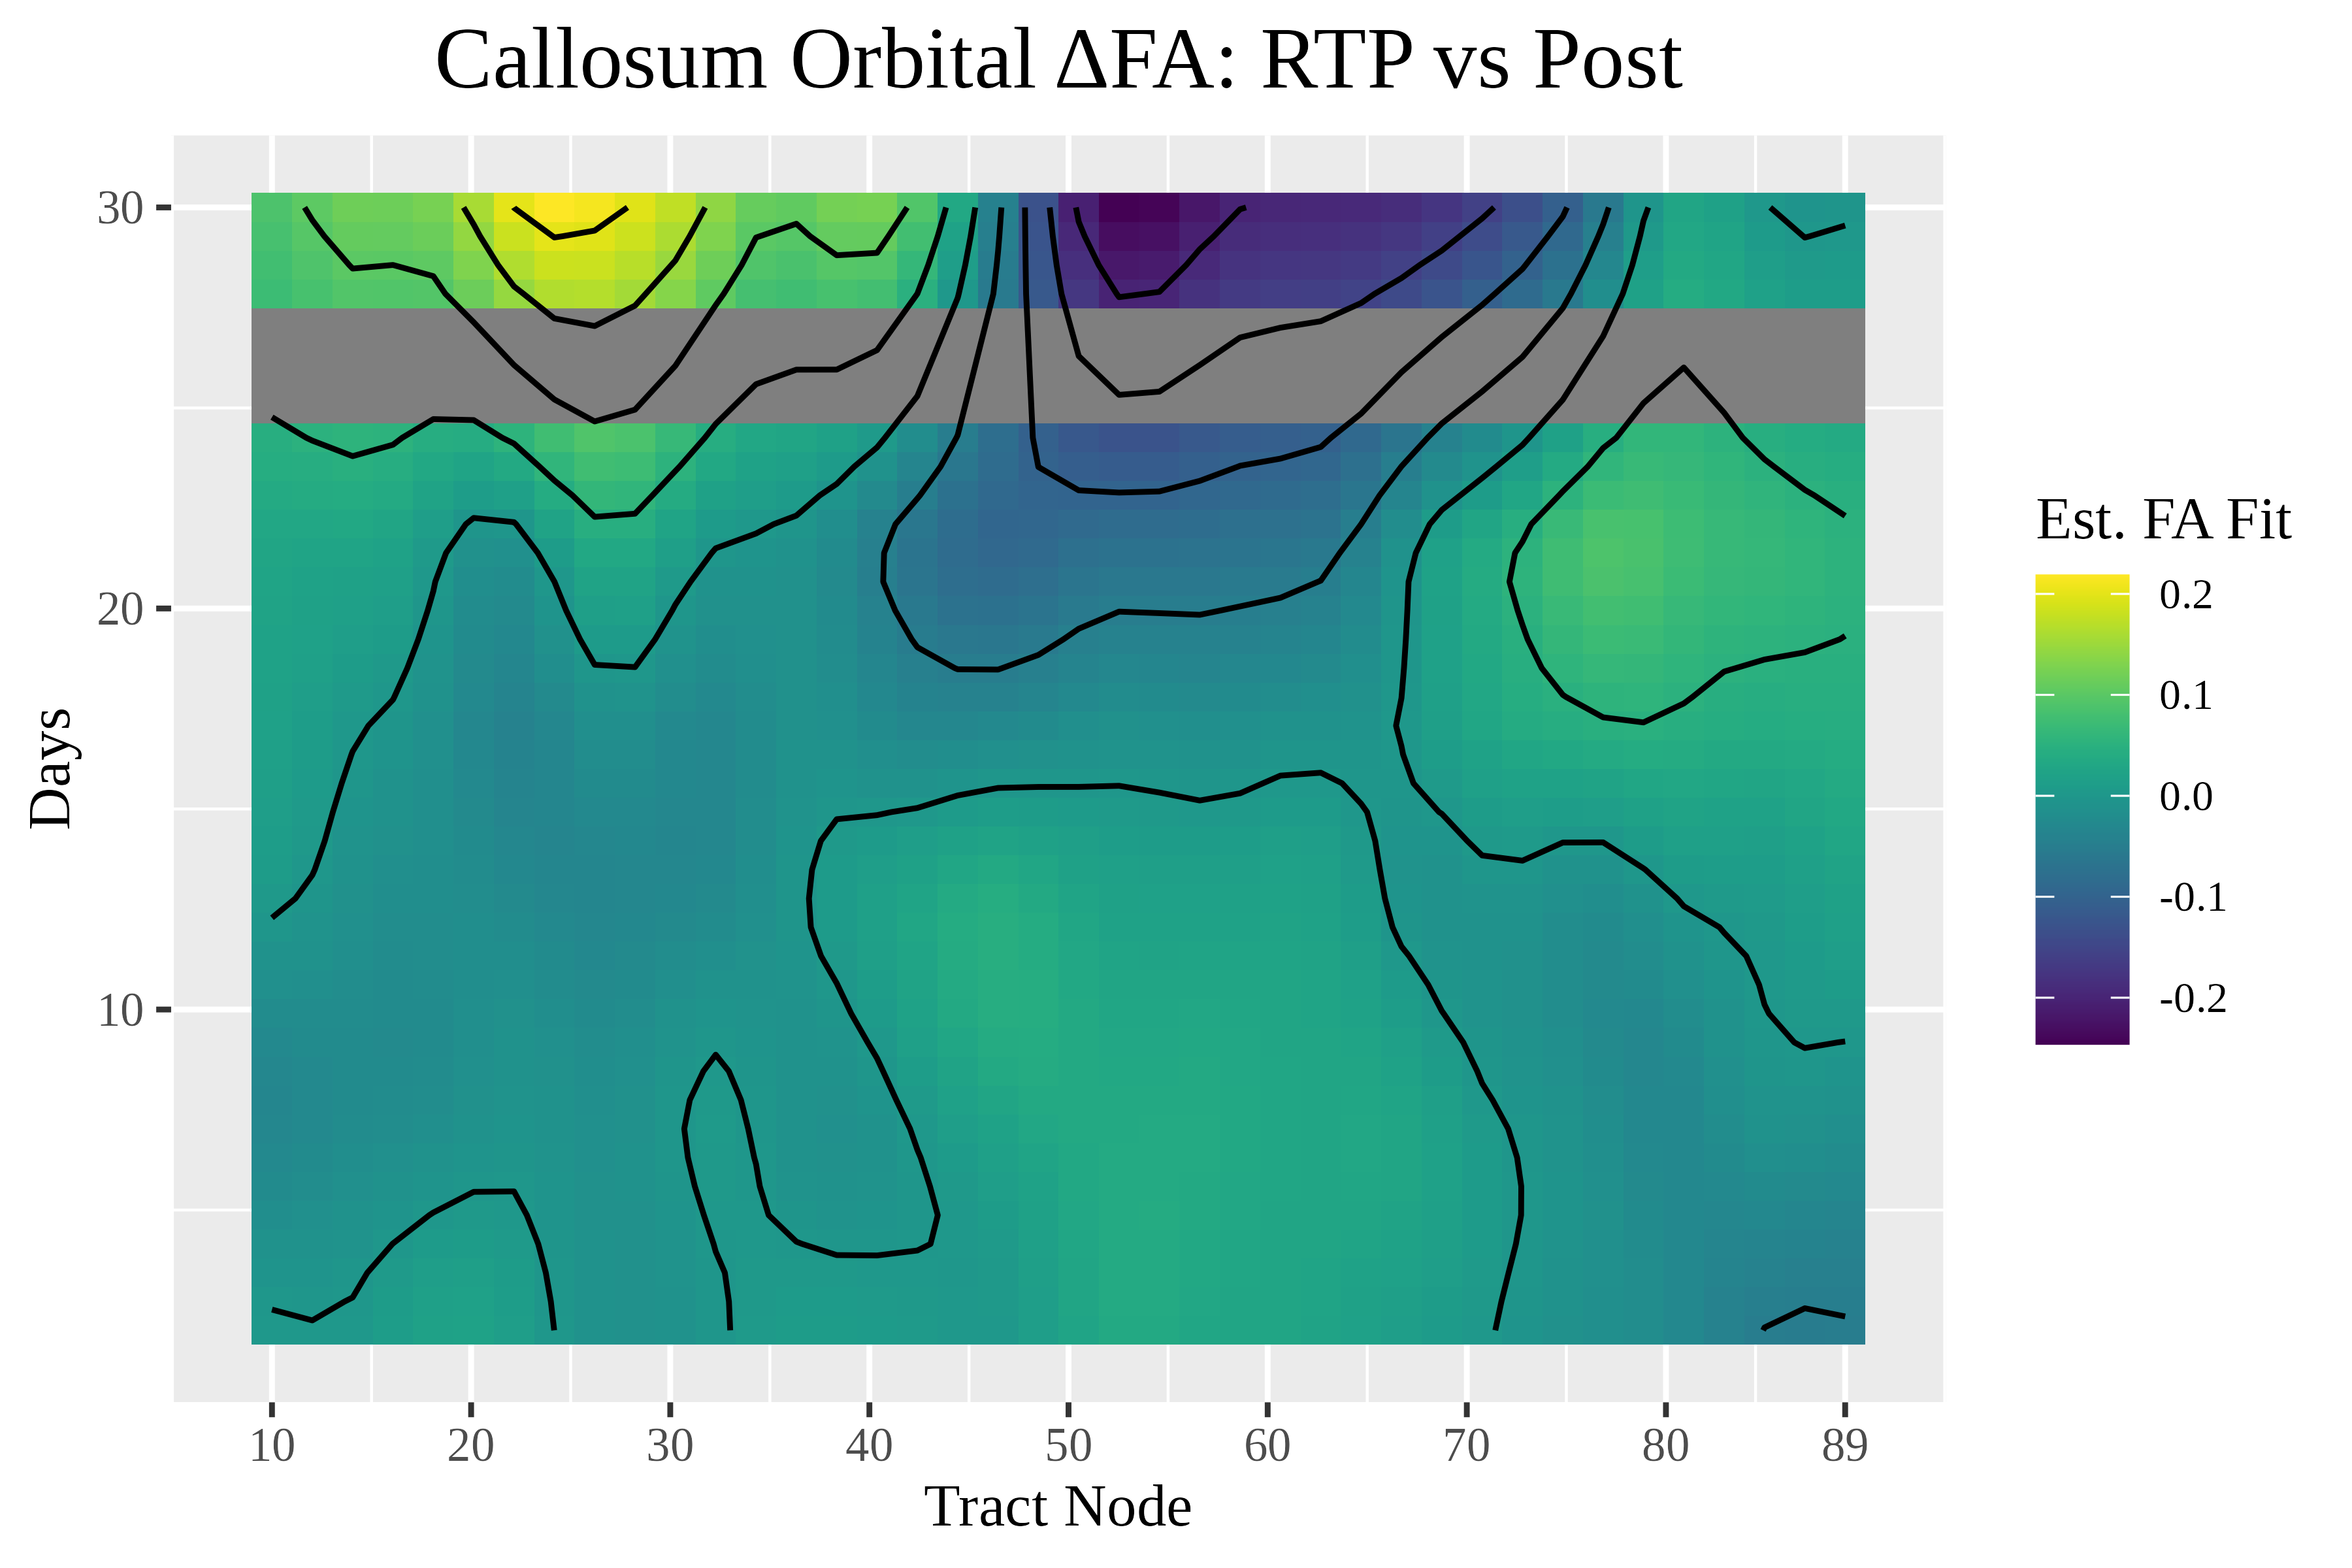
\includegraphics[width=3in]{fit_DI_time_CCorb_fa.png}}
	\captionsetup{} % reset caption specs
	\caption{HGAM tensor product interaction smooths of FA change by recovery time. Interactions are present between RTP-Post $\Delta$FA values (Z-axis), number of days between Post and RTP visits (Y-axis), and tract nodes (X-axis). Positive RTP-Post $\Delta$FA values are indicated as yellow, and negative as blue, with gray bars indicating regions of extrapolation (insufficient data). Top plots indicate positive $\Delta$FA values about node 50 are associated with a larger number of days between Post and RTP, and bottom plots the opposite.}
	\label{fig:di-time}
\end{figure}

First, positive $\Delta$FA values were associated with longer recovery periods in the left corticospinal (node 50) and right uncinate (node 55) tracts (Figure \ref{fig:di-time} a \& b), and negative $\Delta$FA values in the left corticospinal tracts related to a shorter recovery period. Second, negative RTP vs. Post $\Delta$FA values in the callosal superior parietal (node 55) and callosal orbital (node 60) tracts were related to longer recovery periods (Figure \ref{fig:di-time} c \& d). As noted above, injury-related FA changes in this sample have largely been driven by changes in RD, and accordingly the former set of findings may indicate that demyelination deflated FA by increasing RD at Post, resulting in a positive RTP vs. Post $\Delta$FA value, while cellular edema may explain the increased Post FA values of the latter findings due to a decrease of RD (see Discussion). Shorter recovery periods, however, did not have a clear relationship with $\Delta$FA values in these tracts as indicated by the flat (homogeneous green) regions of the tensor product interaction smooths.


\section{Discussion}
\label{sec:disc}
% Recap
Diffusion MRI and ImPACT assessment data were collected from 69 University of Nebraska-Lincoln's NCAA athletes in order to study the effects of concussion on white matter organization. Athletes contributed data at three visits: pre-season (Base), within approximately 48 hours after diagnosed concussion (Post), and after completing the return-to-play protocol (RTP). This prospective, longitudinal dataset is singular, to our knowledge, and facilitates an important step forward in understanding the nature of injury and recovery. Probabilistic tractography generated a set of white matter tracts for each subject and visit, and we employed hierarchical generalized additive models (HGAM) to (a) conduct a longitudinal, whole-brain analysis of injury and recovery, (b) determine the source of FA change, and (c) relate changes in FA values to ImPACT and recovery time. Importantly, this is the first time HGAMs have been used to study concussion injury- and recovery-related tract scalar changes, and we propose that such a technique is critical given their capability of modeling non-linear interactions.

% Findings - scalar changes
\subsection{Scalar Changes Relate to Mechanisms of Injury}
\label{ssec:disc-tract}
In terms of study findings, we first detected within-tract FA changes in hypothesized regions (posterior corpus callosum) which recovered after injury, confirming our first hypothesis. Importantly, we also detected a number of FA changes in other tracts and demonstrated that, in accordance with our second hypothesis, RD was the source of such FA change. Identifying the source of FA change is critical to understanding injury sequelae and recovery as concussion-related changes in AD and RD are associated with different axonal pathologies.

For brief review (see \textcite{krieg2023IdentifyingPhenotypesDiffuse}), the axon is a thin, tubular extension of the neuronal cell body which is composed of the axolemma that anchors to the actin-spectrin complex and, when myelinated, are sheathed by concentric loops of glial lamellar extensions that attach to the cytoskeleton via anchoring proteins. Within the axon, $\alpha$/$\beta$-tubulins form microtubules which are connected with microtubule-associate proteins such as tau. These microtubules form the backbone of the axonal transport system, where transport proteins move mitochondria, vesicles, and other organelles along the axon \parencite{shin2020AxonalTransportDysfunction}. Neurofilaments occupy the space between the central microtubules and the actin-spectrin complex, and their sidearms support the diameter of the axon via electrostatic repulsion and by cross-bridging with neighboring filaments.

%  non/terminal apoptotic caspases can also be activated via increased oxidative stress and [Ca$^{2+}$]i.
With respect to injury, the rapid application of shear, tensile, and/or compressive strains from sports-related de/acceleration injury can have differential effects on the various components of the axon. Initially, excitotoxic activity and physical deformation can result in increased intracellular calcium concentrations ([Ca$^{2+}$]i) through depolarization of the membrane potential, axolemmal mechanoporation, and alterations of ionic channels \parencite{baracaldo-santamaria2022RevisitingExcitotoxicityTraumatic,christman1994UltrastructuralStudiesDiffuse,povlishock1997ImpactAccelerationInjury,pettus1996CharacterizationDistinctSet}. The increased [Ca$^{2+}$]i (via mechanoporation, voltage-gated Ca$^{2+}$ and Na$^+$ channels, AMPA and NMDA receptors, and reversal of Na$^+$-Ca$^{2+}$ exchangers) then triggers secondary injury mechanisms by activating proteolytic calpains which degrade cytoskeletal structures, ionic channels, and receptors \parencite{krieg2023IdentifyingPhenotypesDiffuse}. For instance, activated calpains hydrolyze nodal microtubule-association proteins, degrading the axonal transport system which results in nodal accumulation of transport products, causing swelling \parencite[i.e. varicosities, when stained for $\beta$-amyloid precursor protein][]{ma2013RoleCalpainsInjuryinduced,johnson2013AxonalPathologyTraumatic,shin2020AxonalTransportDysfunction}. Swelling increases tortuosity for intracellular water. Relatedly, increased intracellular osmolarity via excessive glutamatergic activity and disrupted/degraded ionic channels and exchangers draws water into the cell, resulting in cytotoxic edema \parencite{rungta2015CellularMechanismsNeuronal}. Extracellular water, having low tortuosity and relatively unconstrained diffusion, is associated with higher $\lambda_\perp$ values in diffusion MRI metrics while intra-axonal diffusion is both more tortuous and constrained \parencite{mayer2010ProspectiveDiffusionTensor,rosenblum2007CytotoxicEdemaMonitoring}. Nodal swelling into the extracellular space due to cellular or cytotoxic edema accordingly results in lower RD values due to the decrease of extracellular waters.

Further, secondary Ca$^{2+}$-mediated cascades can result in neurofilament compaction. In an uninjured state, phosphorylation of heavy and medium neurofilaments results in their straightening and bundling, supporting the axonal diameter. Injury-related increased [Ca$^{2+}$]i activates both calcineurin and calpain, which dephosphorylate and degrade the filaments, respectively, promoting compaction \parencite{krieg2023IdentifyingPhenotypesDiffuse,pant1988DephosphorylationNeurofilamentProteins,chen1999EvolutionNeurofilamentSubtype}. This compaction increases tortuosity along the axon, decreasing $\lambda_\parallel$, as would axonal undulation and caspase-mediated axotomy \parencite{svandova2023MakingHeadCaspases}. Finally, myelin binding sites near nodes of Ranvier are vulnerable, as are nodal channels, with injury resulting in channel loss, demyelination, and the detection of disassociated key anchoring and structural proteins \parencite{song2022ConcussionLeadsWidespread,zhu2016NodalTotalAxonal,krieg2023IdentifyingPhenotypesDiffuse}. As demyelination occurs, encapsulated water within the sheathes is released into the extracellular space, increasing $\lambda_\perp$ \parencite{mayer2010ProspectiveDiffusionTensor}.

Together, then, $\lambda_\parallel$/AD can be understood to relate to key structural aspects of the axon, with a decrease indicative of severe damage from which the cell may not be able to recover. On the other hand, changes in $\lambda_\perp$/RD relate to intra/extracellular water ratios and their respective differences in tortuosity, which can be driven by cellular or cytotoxic edema and/or demyelination \parencite{borja2018DiffusionMRImaging,mayer2017SpectrumMildTraumatic,lindsey2023DiffusionWeightedImagingMild}. Understanding both is critical when investigating injury-related FA changes as FA is calculated from $\lambda_{1-3}$, where a decrease in FA can result from a lower AD \textit{or} higher RD value. Our first set of findings indicate that the concussion-related FA differences at Post were largely driven by changes to RD and not AD, which is consistent with both the severity of the injury (sport-related concussion or mTBI) and axonal damage from which the cell is able to recover; cellular repair is supported by RTP FA and RD values which returned to baseline. Further, the majority of detected patterns of scalar change (increased FA, decreased RD) are consistent with cellular edema. For tracts which worsened (callosum orbital, left arcuate), the relative pattern of changes were similar: both tracts demonstrated decreased FA and increased RD at RTP (relative to base), a pattern that is consistent with demyelination.


\subsection{FA Relates to ImPACT and Recovery Time}
\label{ssec:disc-impact}
% Findings - scalar and impact interactions
Second, we detected our hypothesized interaction between changes in ImPACT assessment and tract FA values in a number of tracts: the callosum superior frontal FA values related to both the Visual Memory composite and Total Symptom score, callosum occipital to Visual Memory composite, callosum superior parietal to Total Symptom score, and left corticospinal to Reaction Time composite. We note that our hypothesized interaction pattern was only detected in these five instances; while it is possible that a non-linear relationship between node FA values and ImPACT may better capture the nature of injury, or that changes in another scalar would share more variance with ImPACT measures, these were not originally hypothesized, and we found them difficult to understand and justify. We suspect that the lack of hypothesized interactions speak to the limited specificity of ImPACT metrics \parencite{schatz2013SensitivitySpecificityOnline} when studying concussion injury- and recovery-related diffusion changes.

Nevertheless, these multimodal tensor product interaction smooths directly relate clinical diagnostic metrics to within-tract diffusion MRI values, and also help to tease apart injury heterogeneity. Indeed, one difficulty in studying sport-related concussion is the variable nature and location of injury, which constitutes significant inter-individual differences at the group level \parencite{lindsey2023DiffusionWeightedImagingMild}. Accordingly, group-level statistics likely suffer from Type-II errors, where a real but idiosyncratic injury for one athlete is lost in the total variance of the group. The ability to incorporate clinical metrics by modeling data with 2D tensor product interaction smooths help interrogate such group data and may reveal subgroups. For instance, in Figure \ref{fig:lgio-intx-imp}D (top) only individuals with large decreases in FA about node 50 had higher Total Symptom scores, while the tract-FA-ImPACT relationship was rather flat for athletes without such an injury. Additionally, we note that such an interaction is only apparent at the Post visit, during acute injury and poor ImPACT performance (Figure \ref{fig:imp-gam}). By RTP, when ImPACT performance recovers and athletes are cleared for play, the tract-FA-ImPACT relationships do not differ from baseline (Figure \ref{fig:lgio-intx-imp}D, bottom). This pattern of findings, where the hypothesized interaction between tract node FA and ImPACT metric is present at Post and not RTP, extends to all those reported. Given that evidence of recovery from Section \ref{sssec:res-dwi-pat-recov}, we interpret such patterns as, first, evidence that microstructural disruption of axonal processes relate to a decline in ImPACT performance, and second that the lack of such tract-FA-ImPACT interaction at RTP is evidence of recovery.

% Findings - scalar change and recovery time
Third, and finally, we tested whether recovery time was related to the difference in Post and RTP FA values. We reasoned that given all athletes were eventually cleared for return-to-play and that tract scalars were demonstrated to return to Base values, a larger RTP-Post $\Delta$FA would be driven by more severe injury sequelae at Post and that such injuries would necessitate longer recovery periods. The tensor product interaction smooths of Figure \ref{fig:di-time} demonstrate a linear relationship between FA change and recovery time in the left corticospinal, right uncinate, callosum superior parietal, and callosum orbital tracts. Within these tracts, two patterns were detected: positive $\Delta$FA values related to longer recovery periods in the corticospinal and uncinate tracts (Figure \ref{fig:di-time}, top), presumably driven by RD increase due to demyelination at Post, and the reverse in callosal superior parietal and orbital tracts (Figure \ref{fig:di-time}, bottom) which may be caused by RD reduction due to cellular or cytotoxic edema. Such findings provide insight into variance in recovery trajectories, and we note that tensor product interaction smooths would be well employed to longitudinally study recovery if multiple scans were acquired during the recovery period. Additionally, it would be possible to include other factors which may relate to recovery (e.g. metrics of cardiovascular exercise or number of previous TBIs) to determine the amount of shared variance in recovery.


\subsection{Limitations}
\label{ssec:disc-limit}
While HGAMs provide a powerful statistical approach to model within-tract scalar values across groups or time, we note six limitations in our implementation. First, we elected to start with a longitudinal, whole-brain model which incorporated all tracts from each participant across all visits in order to capture any shared variance of injury which spanned multiple tracts. In specifying such a model, each tract was provided with the same maximum basis dimension, a parameter which controls the `wiggliness' of the smooth. As tractometric profiles differ in their curvature, such a specification may have resulted in underfitting certain tracts. While a review of each tract, and models specific for each tract, indicated that a basis dimension of 15 was sufficient, future models may require fine-tuning this parameter. Second, interpreting smooths for significance versus evidence about the intended hypothesis can be an involved process. Here, we used HGAMs to investigate concussion-related injury and recovery, and selected models around a central hypothesis that post-injury tractometric profiles and their corresponding smooths, but not those for return-to-play, would differ from baseline. GAMs test against the null hypothesis, however, that the best fit of the interaction is a flat smooth, or, that increasing the effective degrees of freedom (wiggliness) does not improve model fit. Accordingly, simply modeling a tract profile would result in significant models given the curvature of the node-scalar interaction. To account for this, we both employed HGAMs which enabled us to hold constant the tract curvature (global smooth) and ordinal factors (Base $<$ Post $<$ RTP) to derive test statistics that related to our hypotheses. Third, in addition to the `significance' of the statistic, it is critical to consider the magnitude of the effect, and an a priori idea of the shape of the smooth is warranted when investigating complex interactions. While smooths are penalized to reduce overfitting, small deflections from flatness can result in statistical, but not practical, significance. To guard against this, we interrogated the magnitude of the partial effects for the smooths of interest, often with respect to the global smooth, and started with defined hypotheses of the deformation pattern in tensor product interaction smooths. Nevertheless, we considered certain effects as not (practically) significant, such as the RTP vs. Base interaction smooths, while their corresponding p-values were less than the criterion $\alpha$ = .05, and note that in such cases both the effective degrees of freedom and F-statistics were reduced. Fourth, the statistic of tensor product interaction smooths can be driven by sparsity: when investigating the interaction of RTP vs. Post $\Delta$FA and recovery time, relatively few athletes had recovery times longer than 14 days and may have driven the deflections from flatness (particularly in Figure \ref{fig:di-time} C \& D). We nevertheless included these results as we considered such models to be instructive. Fifth, sport-related concussion is a category of injury that is defined by its heterogeneity and accordingly group-level statistics lack sensitivity. We initially sought to identify subgroups within our sample, which would allow for a double-dissociation approach to studying tractometric changes, but our sample was too uniform in their ImPACT composites to identify clusters. Larger datasets would likely have a number of subgroups which would allow for the better interrogation of the relationship between structural changes and clinical response. Finally, while we quantified the contribution of algorithmic (run-rerun) variance, it is relevant to consider scan-rescan variance when studying mTBI with diffusion weighted imaging. Modern, faster protocols that allow for multiple scan acquisitions during a single visit (e.g. \cite{li2020EvaluationMultishellDiffusion}) will account for some inherent thermal noise as multiple measures of each diffusion direction can be combined and averaged.


\subsection{Conclusions}
\label{ssec:disc-conc}
The present study demonstrates that HGAMs are well-suited to sensitively model within-tract diffusion changes that relate to concussion injury and recovery. Their ability to model non-linear interactions provides a better fit to complex data than traditional approaches, facilitating the detection of subtle group-related changes. Further, longitudinal or group-difference models are facilitated by incorporating a nested factor structure, and higher dimensional multimodal models allow for the interrogation of clinical import. Here, we employed HGAMs to demonstrate that concussion injury- and recovery-related scalar changes were present in a number of commissural and association tracts, that radial and not axial diffusivity was the source of fractional anisotropy change, and that such changes related to both clinical metrics and recovery duration.


% acknowledgment page
\section*{Acknowledgments}
\label{sec:ack}
The authors thank Ariana M. Hedges-Muncy for statistical consults, and the following people for their help with MRI data acquisition: Ruby Basyouni, Elliot Carlson, Mark Mayer, Joanne Murray, and Julie Tuttle.

This work was supported by a grant awarded to MN by the National Institute of Health (NIH) Great Plains IDeA-CTR Network, Pilot Grant Program (2018-2020) "Brain connectivity for prediction of lesion site in sports-related concussion".


% write bibliography
\pagebreak
\printbibliography
\pagebreak


% make supplemental
\section{Supplemental Materials}
\label{sec:supp-materials}
\beginsupplement

\subsection{R Code}
\label{ssec:supp-rcode}

\begin{equ}[H]
	\begin{lstlisting}
		fit_LGI <- mgcv::bam(
		  <scalar> ~ s(subj_id, scan_name, bs="re") +
		    s(node_id, bs="tp", k=15, m=2) +
		    s(node_id, by=scan_name, bs="tp", k=15, m=1),
		  data=df,
		  family=<family>,
		  method="fREML",
		  nthreads=4
		)
	\end{lstlisting}
	\caption{Tract scalars are modeled as a function of tract node with thin-plate regression splines using both global and group (\lstinline{scan_name}) smooths as well as individual group wiggliness. \lstinline{<scalar>} = relevant DWI metric (AD, RD, MD, or FA), \lstinline{scan_name} = visit identifier factor (Base, Post, RTP), \lstinline{<family>} = relevant family and link function for scalar distribution.}
	\label{supp-code:gam-lgi}
\end{equ}


\begin{equ}[H]
	\begin{lstlisting}
		fit_LGI_intx <- mgcv::bam(
		  <scalar> ~ s(subj_id, scan_name, bs="re") +
		    s(node_id, bs="tp", k=15, m=2) +
		    s(imp_meas, by=scan_name, bs="tp", k=5) +
		    ti(
		      node_id, imp_meas, by=scan_name,
		      bs=c("tp","tp"), k=c(20,5), m=1
		    ),
		  data=df,
		  family=<family>,
		  method="fREML",
		  nthreads=4
		)
	\end{lstlisting}
	\caption{Tract scalars are modeled as a function of separate 1D node and ImPACT smooths as well as a 2D tensor product interaction surface. \lstinline{imp_meas} = ImPACT composite or total symptom measure.}
	\label{supp-code:gam-lgi-intx}
\end{equ}


\begin{equ}[H]
	\begin{lstlisting}
		fit_G <- mgcv::bam(
		  imp_meas ~ s(subj_id, bs="re") +
		    s(num_assess, bs="tp", k=3),
		  data=df,
		  family=<family>,
		  method="fREML"
		)
	\end{lstlisting}
	\caption{ImPACT metrics modeled as a function of number of assessments using a single global smooth. \lstinline{imp_meas} = ImPACT composite or total symptom score, \lstinline{num_assess} = assessment number (1=Base, 2=Post, 3=RTP).}
	\label{supp-code:gam-impact}
\end{equ}


\begin{equ}[H]
	\begin{lstlisting}
		fit_DI <- mgcv::bam(
		  delta_fa ~ s(subj_id, by=tract_name, bs="re") +
		    s(node_id, by=tract_name, bs="tp", k=15) +
		    tract_name,
		  data=df,
		  family=gaussian(),
		  method="fREML",
		  nthreads=12
		)
	\end{lstlisting}
	\caption{Run-Rerun $\Delta$FA values were modeled with node smooths for each tract.}
	\label{supp-code:gam-di}
\end{equ}


\subsection{Tables}
\label{ssec:supp-tables}
\begin{table}[H]
	\scriptsize
	% Please add the following required packages to your document preamble:
% \usepackage[table,xcdraw]{xcolor}
% Beamer presentation requires \usepackage{colortbl} instead of \usepackage[table,xcdraw]{xcolor}

\begin{tabular}{lllllllll}
\multicolumn{1}{c}{ImPACT} & \multicolumn{1}{c}{Visit} & \multicolumn{1}{c}{Min} & \multicolumn{1}{c}{Q1} & \multicolumn{1}{c}{Med} & \multicolumn{1}{c}{Q2} & \multicolumn{1}{c}{Max} & \multicolumn{1}{c}{Skew} & \multicolumn{1}{c}{Kurt} \\ \hline
 & \multicolumn{1}{l|}{Base} & 41.00 & 79.00 & 88.00 & 94.00 & 100.00 & -1.46 & 5.11 \\
VerMem & \multicolumn{1}{l|}{\cellcolor[HTML]{C0C0C0}Post} & \cellcolor[HTML]{C0C0C0}48.00 & \cellcolor[HTML]{C0C0C0}74.75 & \cellcolor[HTML]{C0C0C0}84.50 & \cellcolor[HTML]{C0C0C0}96.00 & \cellcolor[HTML]{C0C0C0}100.00 & \cellcolor[HTML]{C0C0C0}-0.64 & \cellcolor[HTML]{C0C0C0}2.38 \\
 & \multicolumn{1}{l|}{RTP} & 37.00 & 83.25 & 92.00 & 96.00 & 100.00 & -2.01 & 6.65 \\
\rowcolor[HTML]{EFEFEF}
 & \multicolumn{1}{l|}{\cellcolor[HTML]{EFEFEF}Base} & 43.00 & 68.00 & 77.00 & 88.00 & 99.00 & -0.58 & 2.80 \\
\rowcolor[HTML]{C0C0C0}
\cellcolor[HTML]{EFEFEF}VisMem & \multicolumn{1}{l|}{\cellcolor[HTML]{C0C0C0}Post} & 29.00 & 59.00 & 72.00 & 81.50 & 97.00 & -0.59 & 2.85 \\
\rowcolor[HTML]{EFEFEF}
 & \multicolumn{1}{l|}{\cellcolor[HTML]{EFEFEF}RTP} & 43.00 & 71.25 & 78.00 & 83.25 & 97.00 & -0.75 & 3.14 \\
 & \multicolumn{1}{l|}{Base} & 20.82 & 33.30 & 39.65 & 43.25 & 51.50 & -0.22 & 2.59 \\
VisMot & \multicolumn{1}{l|}{\cellcolor[HTML]{C0C0C0}Post} & \cellcolor[HTML]{C0C0C0}18.40 & \cellcolor[HTML]{C0C0C0}34.34 & \cellcolor[HTML]{C0C0C0}37.88 & \cellcolor[HTML]{C0C0C0}45.31 & \cellcolor[HTML]{C0C0C0}51.33 & \cellcolor[HTML]{C0C0C0}-0.54 & \cellcolor[HTML]{C0C0C0}2.73 \\
 & \multicolumn{1}{l|}{RTP} & 19.82 & 36.70 & 40.28 & 47.86 & 51.90 & -0.65 & 3.40 \\
\rowcolor[HTML]{EFEFEF}
 & \multicolumn{1}{l|}{\cellcolor[HTML]{EFEFEF}Base} & 0.48 & 0.56 & 0.61 & 0.69 & 0.87 & 0.65 & 3.18 \\
\rowcolor[HTML]{C0C0C0}
\cellcolor[HTML]{EFEFEF}RxTime & \multicolumn{1}{l|}{\cellcolor[HTML]{C0C0C0}Post} & 0.46 & 0.58 & 0.63 & 0.73 & 1.17 & 1.27 & 4.57 \\
\rowcolor[HTML]{EFEFEF}
 & \multicolumn{1}{l|}{\cellcolor[HTML]{EFEFEF}RTP} & 0.43 & 0.53 & 0.57 & 0.65 & 1.17 & 2.06 & 7.57 \\
 & \multicolumn{1}{l|}{Base} & 1.00 & 3.00 & 6.00 & 9.00 & 30.00 & 1.81 & 7.14 \\
ImpCtl & \multicolumn{1}{l|}{\cellcolor[HTML]{C0C0C0}Post} & \cellcolor[HTML]{C0C0C0}0.00 & \cellcolor[HTML]{C0C0C0}3.00 & \cellcolor[HTML]{C0C0C0}5.50 & \cellcolor[HTML]{C0C0C0}11.25 & \cellcolor[HTML]{C0C0C0}23.00 & \cellcolor[HTML]{C0C0C0}0.84 & \cellcolor[HTML]{C0C0C0}3.13 \\
 & \multicolumn{1}{l|}{RTP} & 1.00 & 4.00 & 6.50 & 10.00 & 18.00 & 0.51 & 2.54 \\
\rowcolor[HTML]{EFEFEF}
 & \multicolumn{1}{l|}{\cellcolor[HTML]{EFEFEF}Base} & 0.00 & 1.00 & 5.00 & 12.00 & 45.00 & 1.62 & 5.94 \\
\rowcolor[HTML]{C0C0C0}
\cellcolor[HTML]{EFEFEF}TotSymp & \multicolumn{1}{l|}{\cellcolor[HTML]{C0C0C0}Post} & 0.00 & 0.00 & 10.50 & 27.50 & 69.00 & 1.05 & 3.06 \\
\rowcolor[HTML]{EFEFEF}
 & \multicolumn{1}{l|}{\cellcolor[HTML]{EFEFEF}RTP} & 0.00 & 0.00 & 0.00 & 3.25 & 35.00 & 2.00 & 5.64
\end{tabular}

	\caption{Descriptive statistics for ImPACT composite and total symptom metrics, by visit. Min = minimum value, Q1 = first quartile, Med = median, Q3 = third quartile, max = maximum value, Skew = skewness, Kurt = Kurtosis. VerMem = verbal memory, VisMem = visual memory, VisMot = visual motor, RxTime = reaction time, ImpCtl = impulse control, TotSymp = Total Symptom.}
	\label{supp-tbl:imp-desc}
\end{table}


\subsection{Figures}
\label{ssec:supp-figures}

\begin{figure}[H]
	\centering
	\subfloat{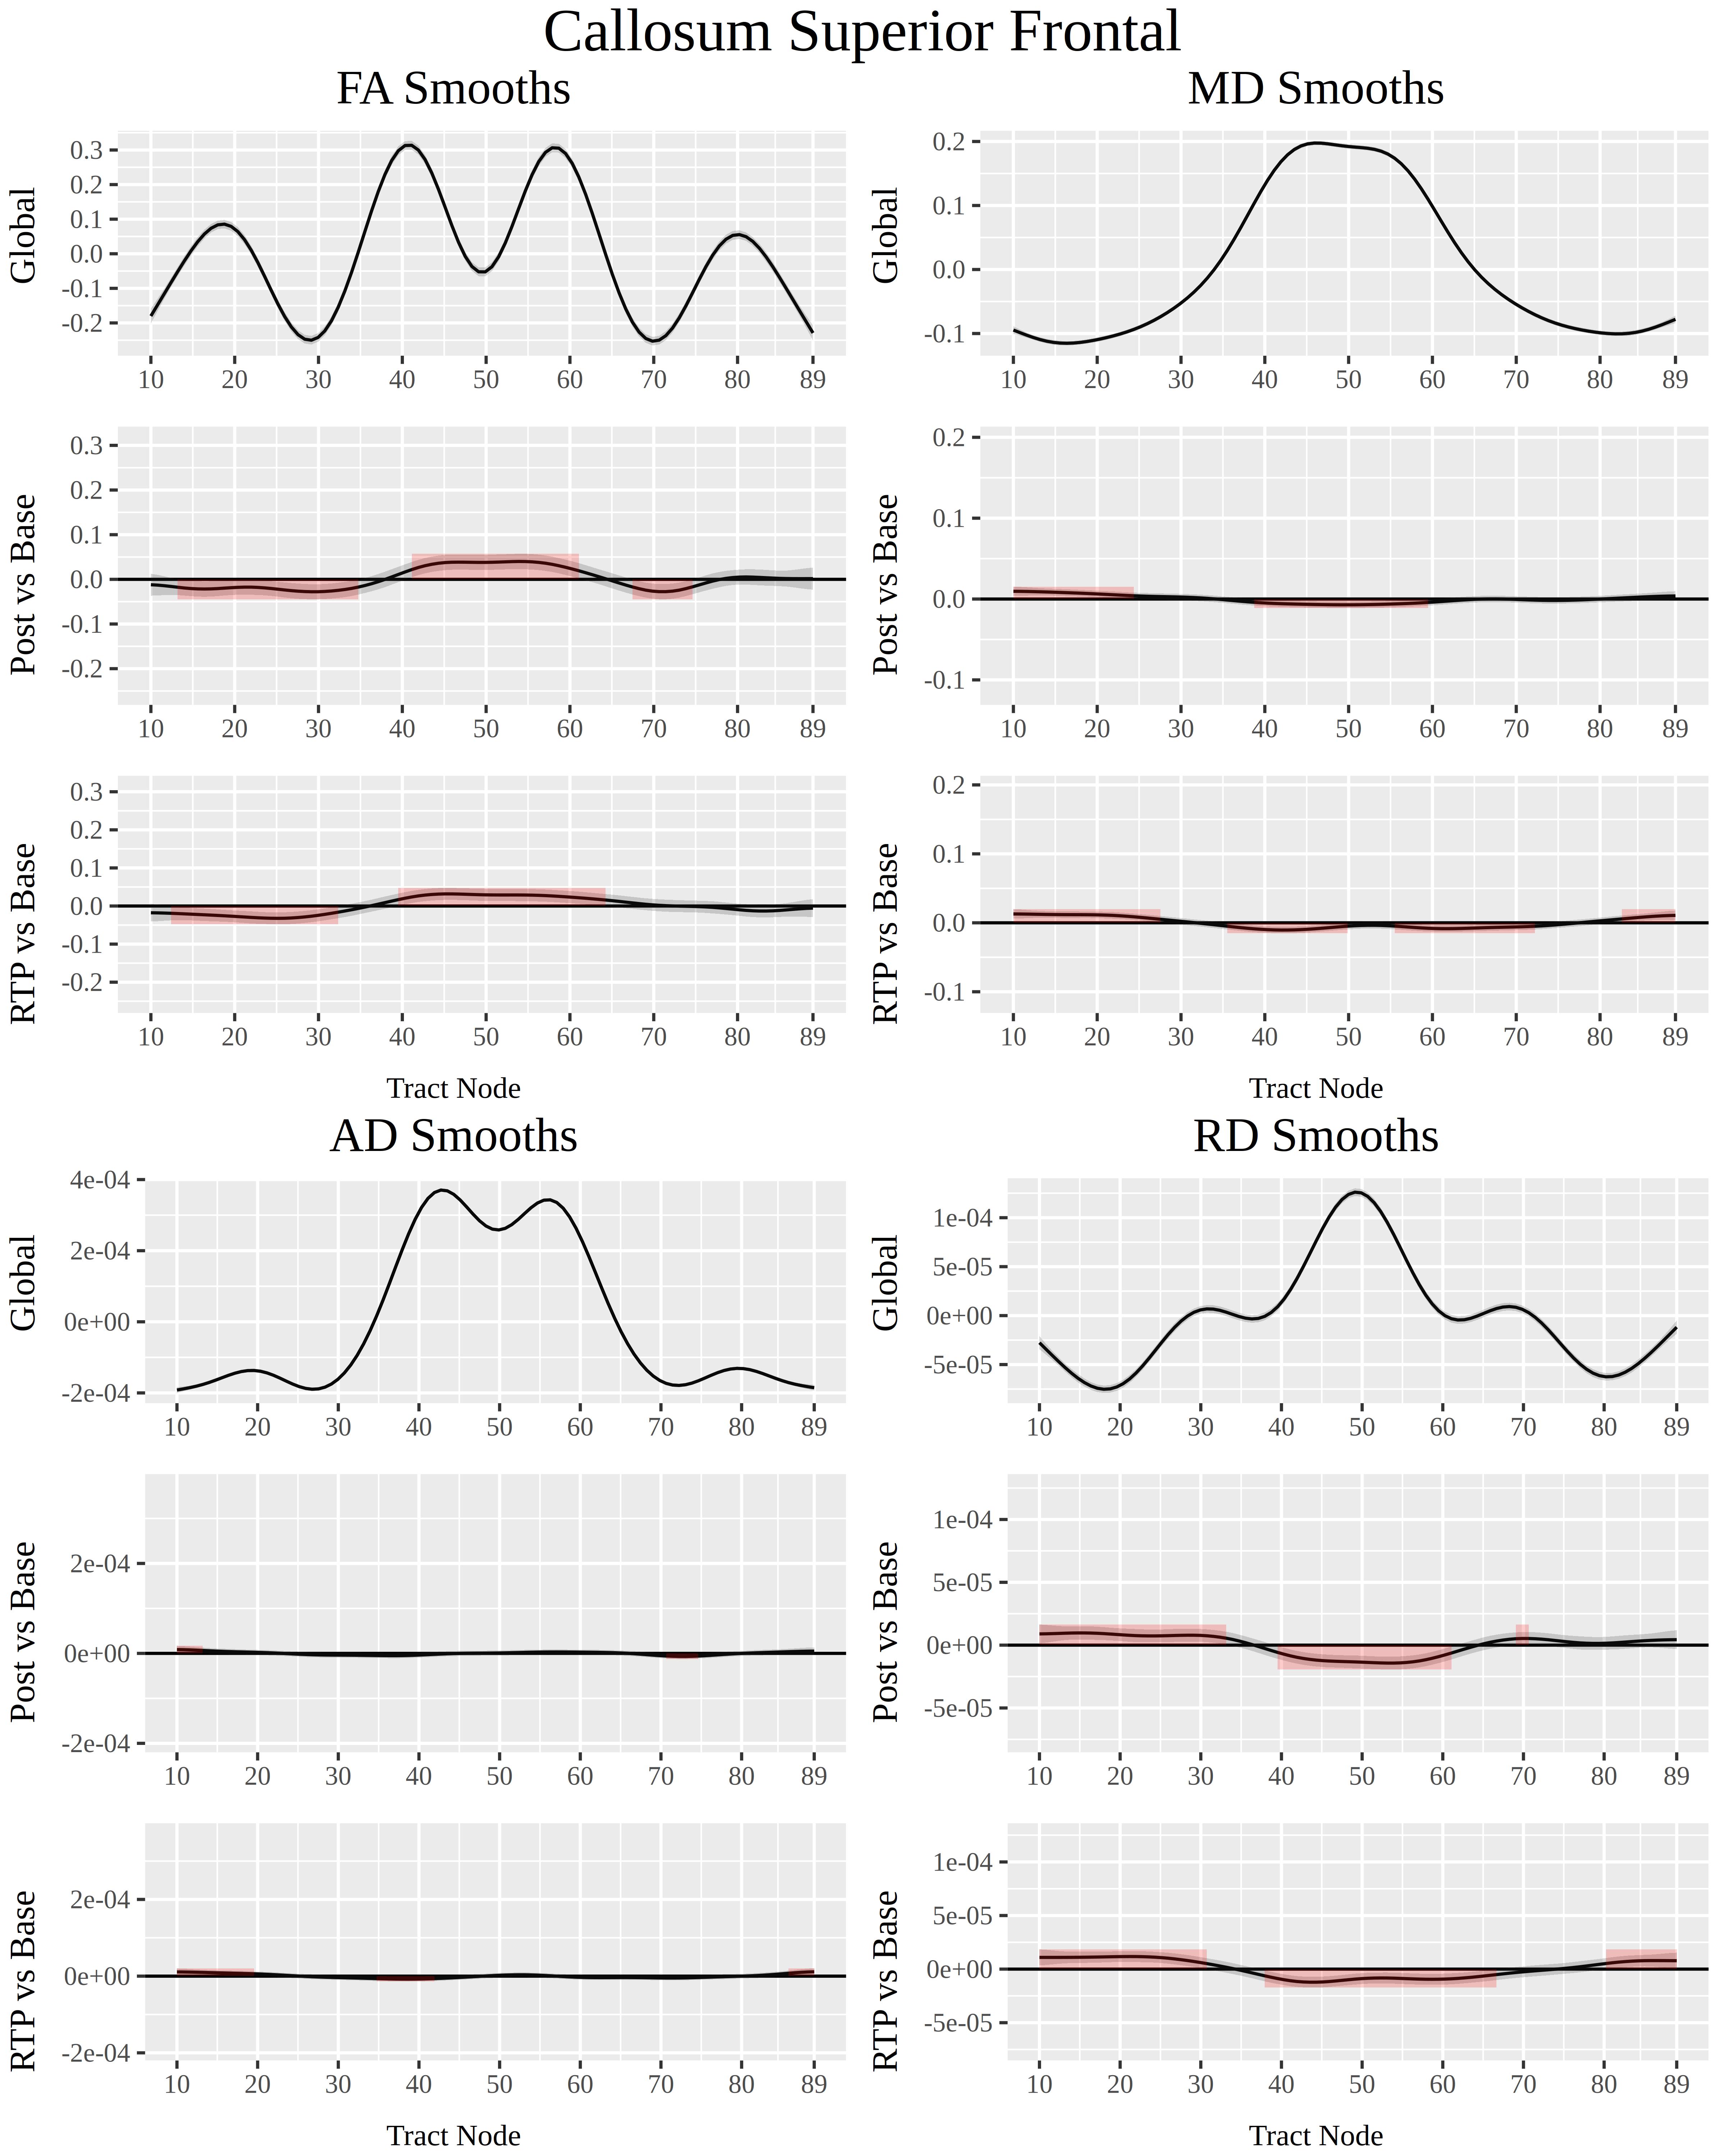
\includegraphics[width=.5\linewidth]{fit_LGIO_CCsf.png}}
	\caption{FA smooths show evidence of Post injury and RTP recovery about node 50. Such changes in FA are driven by RD in the same node region. Some evidence of injury in the right hemisphere (nodes 10-50) is also present.}
	\label{supp-fig:lgio-gam-recov}
\end{figure}

\begin{figure}[H]
	% \captionsetup{labelformat=empty,oneside,margin={-70mm,0cm},captionskip=-98mm} % Use for splitting caption
	\captionsetup{margin={-70mm,0cm},captionskip=-98mm} % Align a-d with top left corner
	\subfloat[]{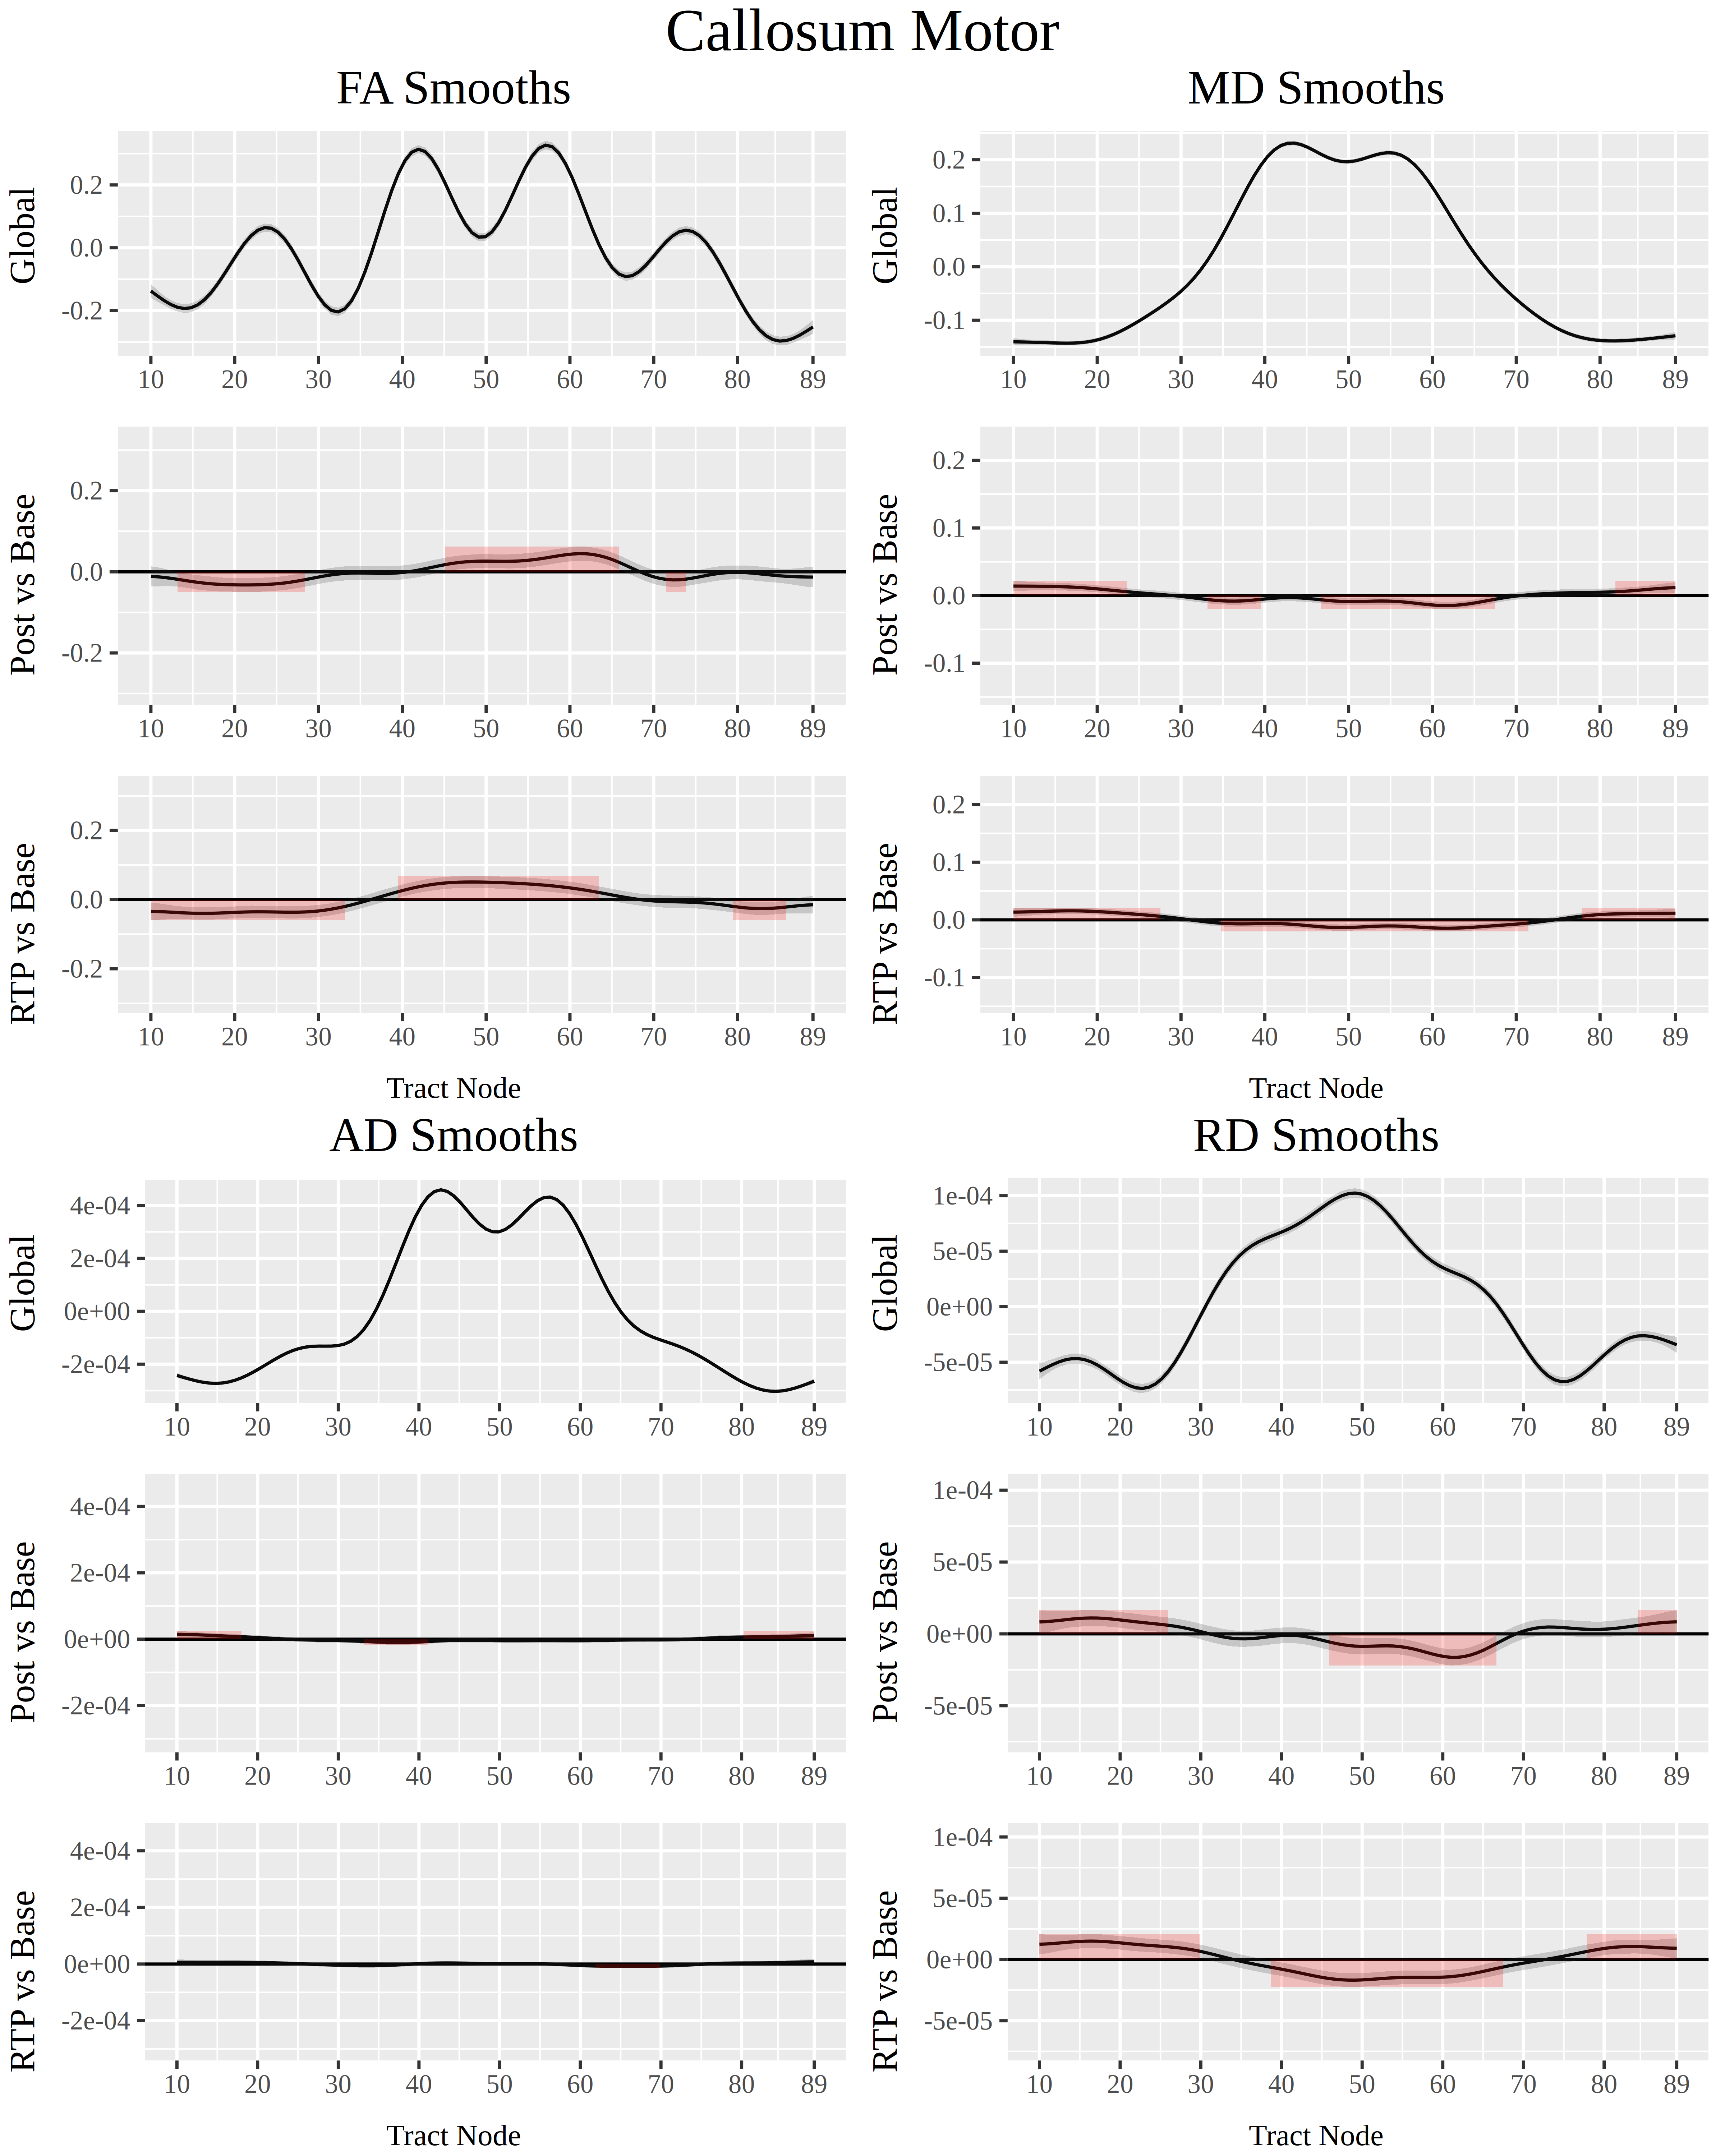
\includegraphics[width=3in]{fit_LGIO_CCmot.png}}
	\subfloat[]{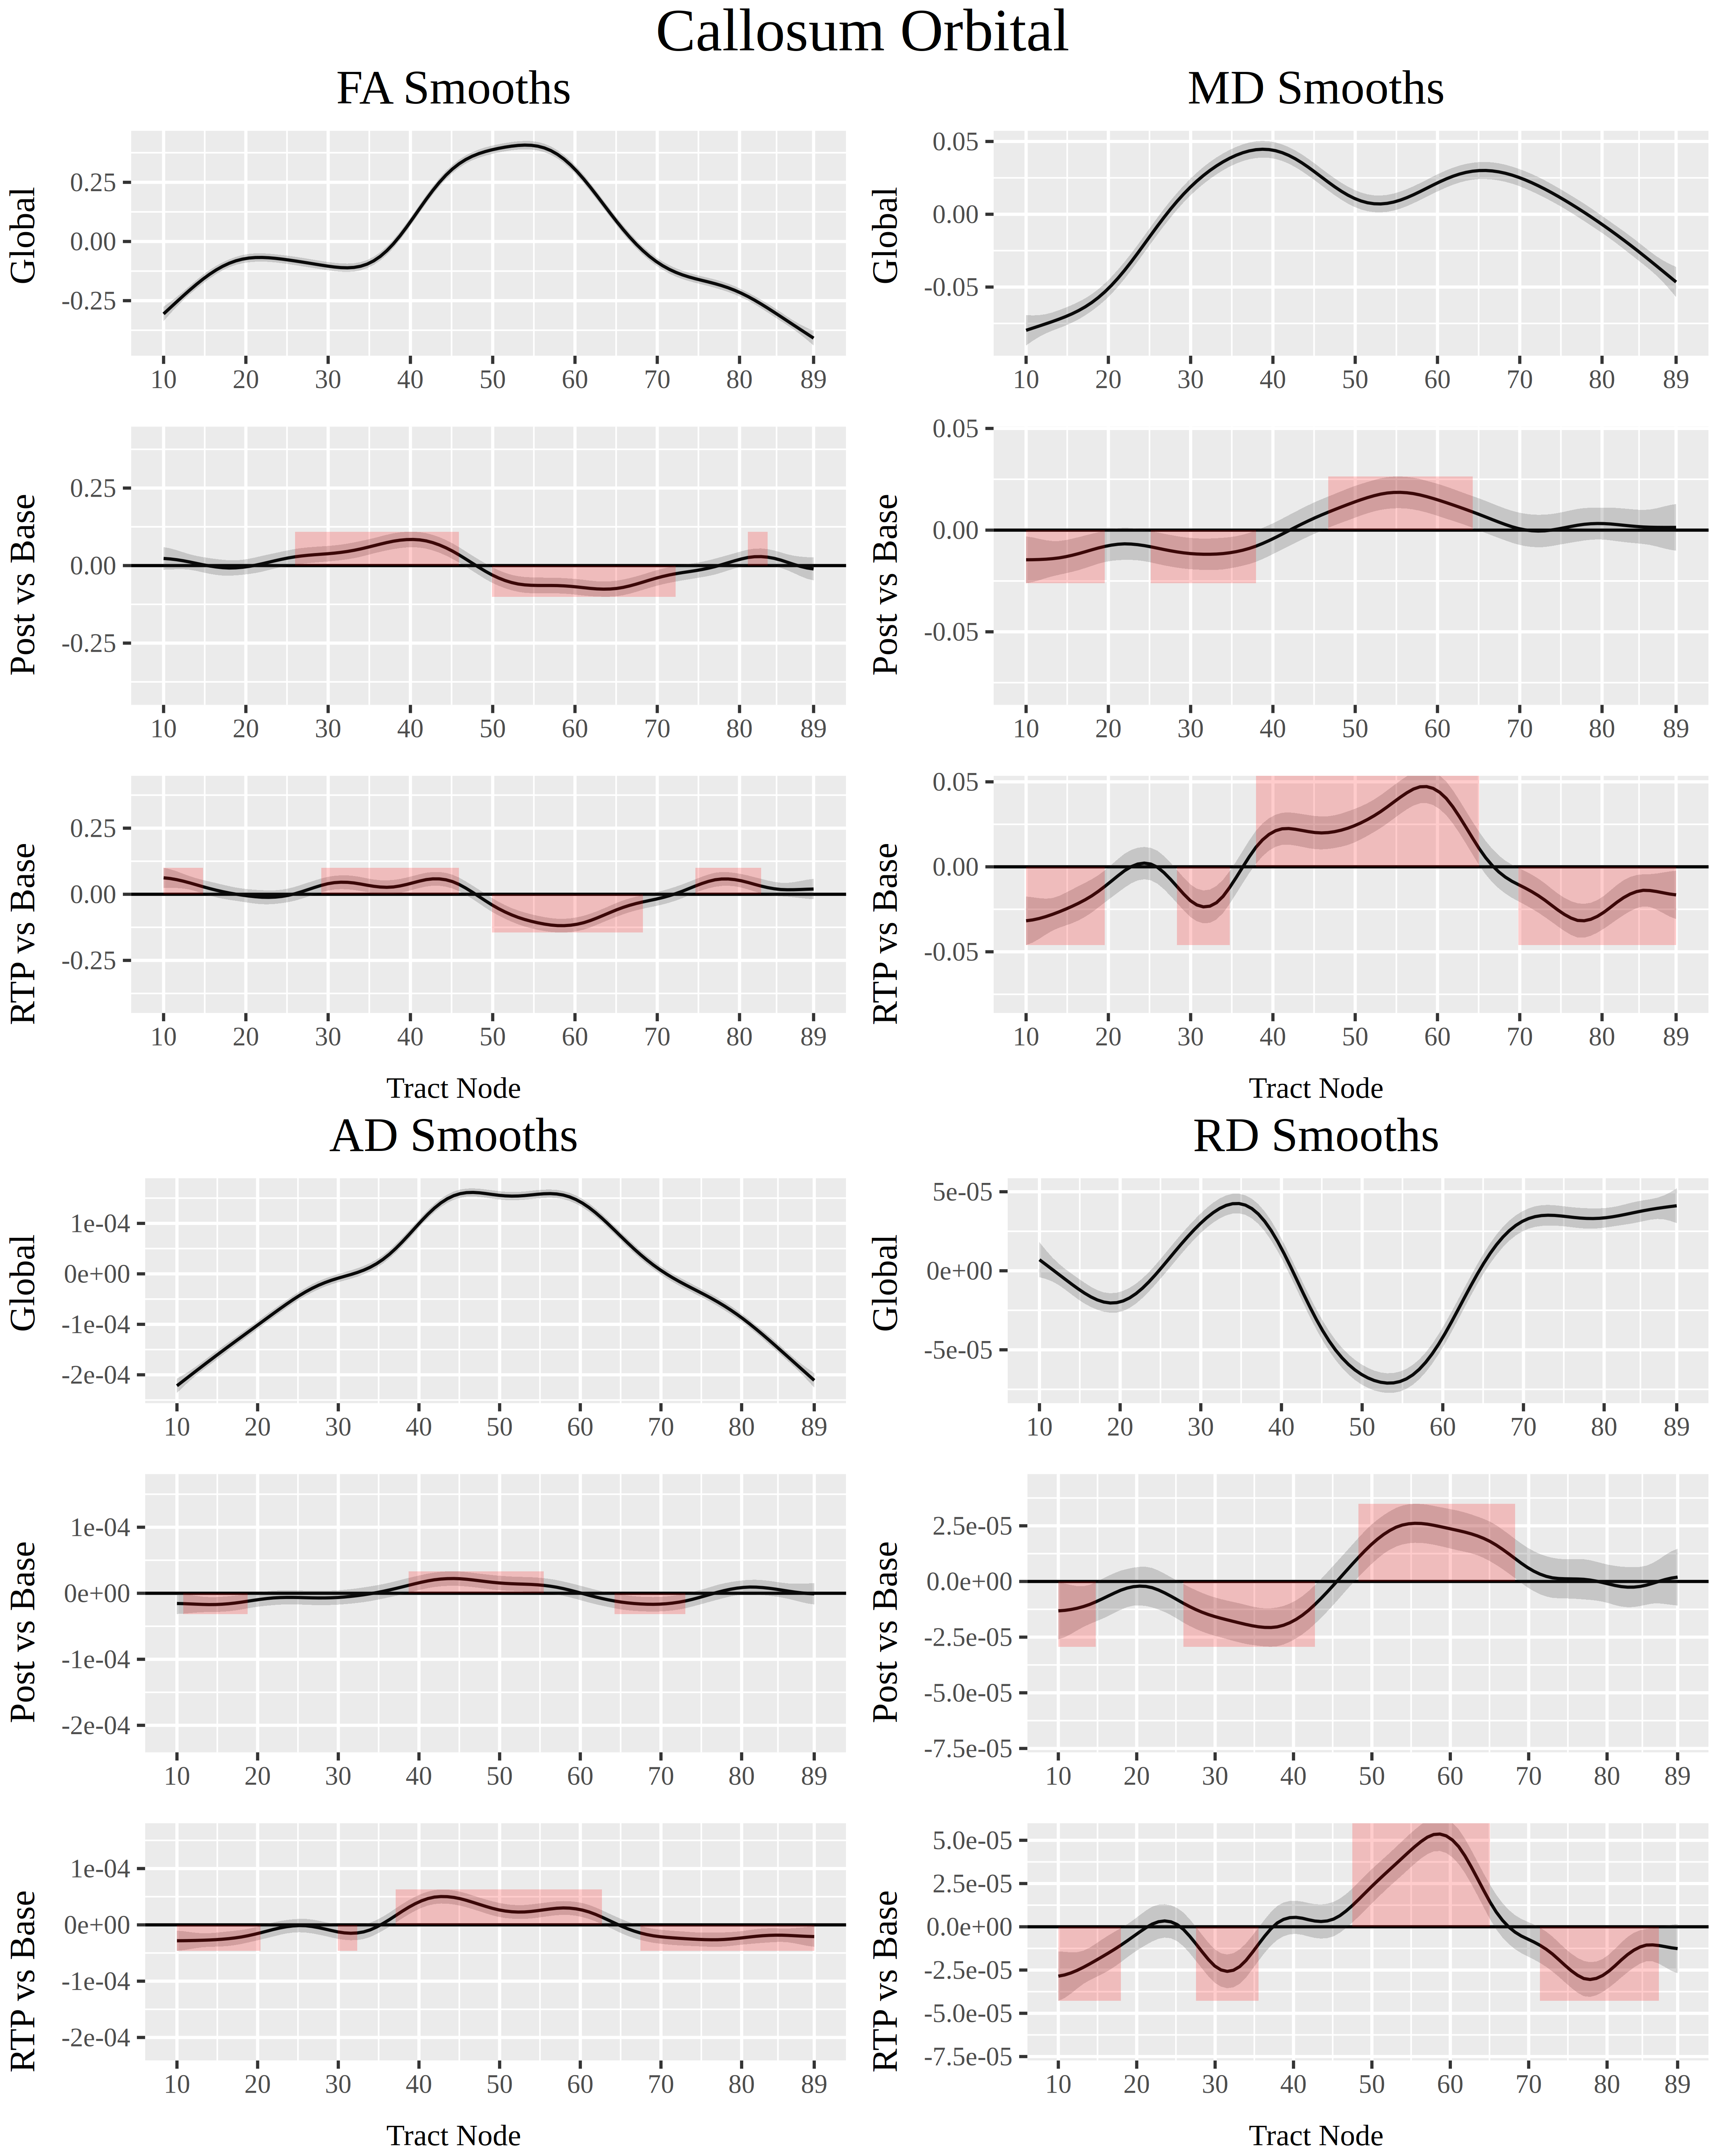
\includegraphics[width=3in]{fit_LGIO_CCorb.png}}\\
	\subfloat[]{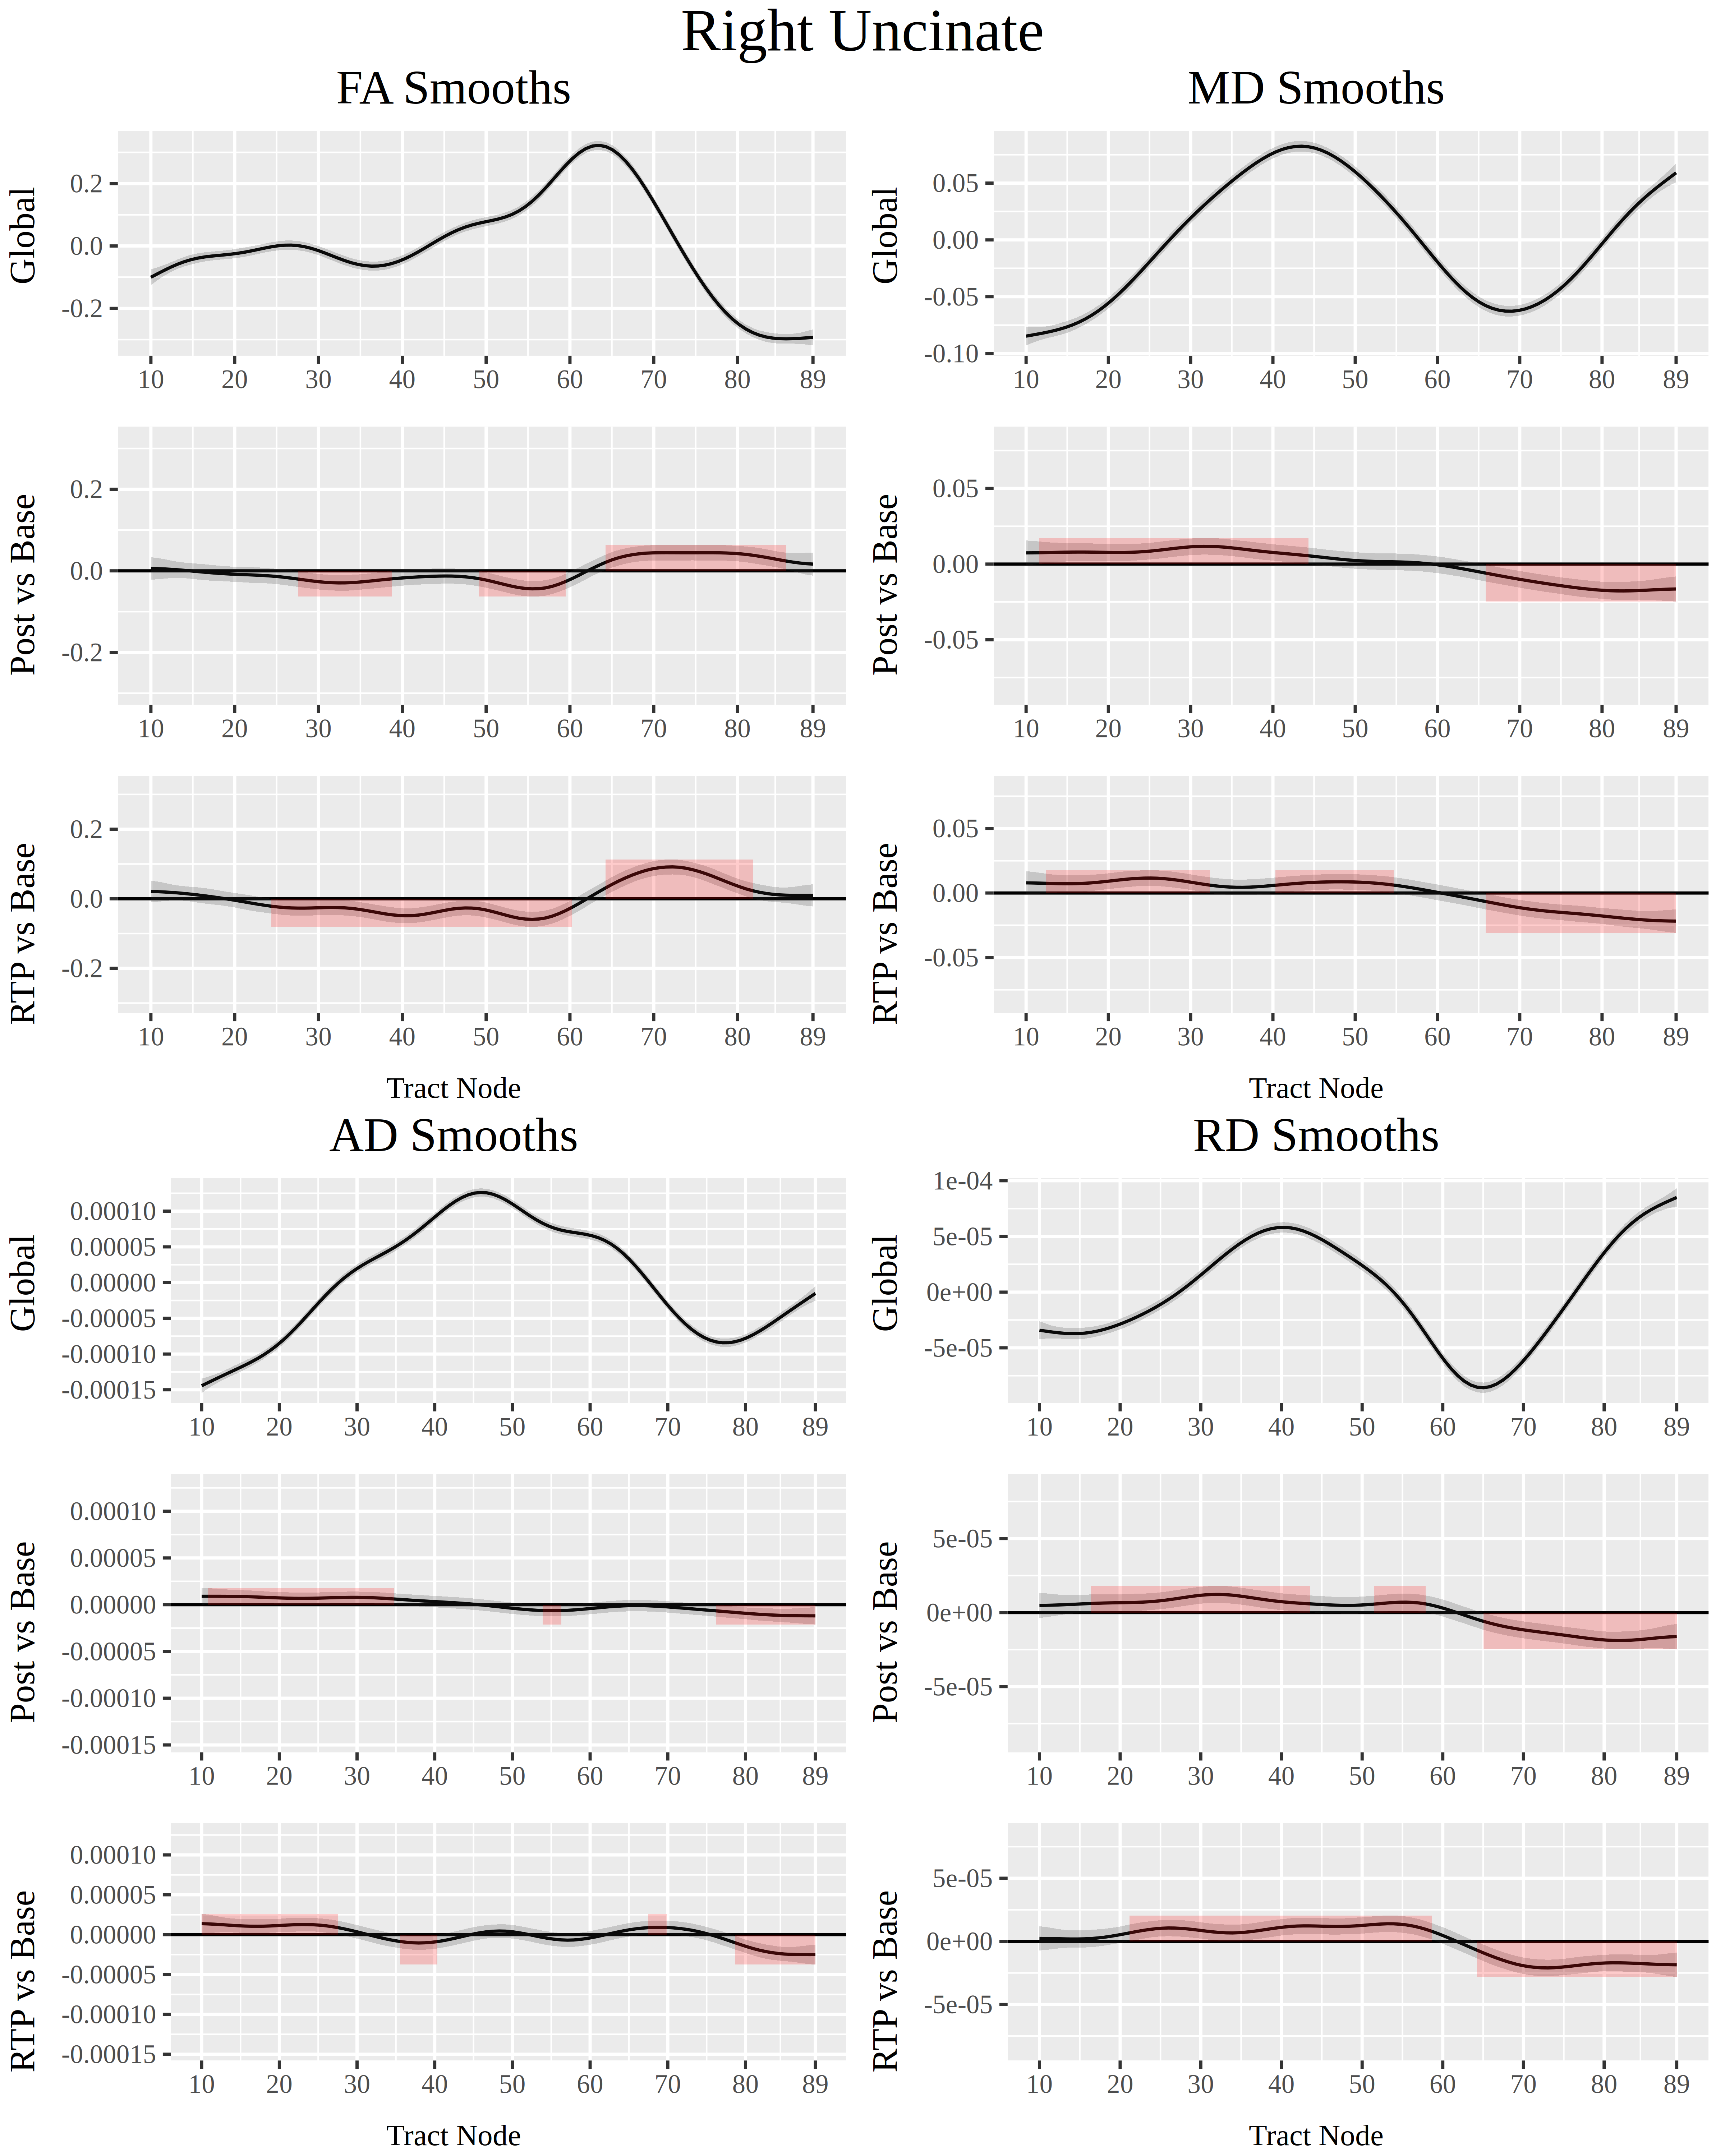
\includegraphics[width=3in]{fit_LGIO_rUnc.png}}
	\captionsetup{margin={0mm,0cm}}
	\caption{(a) Callosum motor shows injury progression about node 60, with increased FA and decreased RD. (b) Callosum orbital has a complex injury profile, with FA decreases (and RD increases) about node 60, and the reverse around node 40. RTP vs. Base AD values are also increased in the parasagittal region (node 50). (c) Right uncinate shows a similar injury profile as callosum motor, with increased FA values about node 70, driven by decreased RD, and the reverse around node 40.}
	\label{supp-fig:lgio-gam-prog}
\end{figure}
% \clearpage
% \begin{figure}
% 	\captionsetup{labelformat=adja-page}
% 	\ContinuedFloat
% 	\caption{(a) Callosum motor shows injury progression about node 60, with increased FA and decreased RD. (b) Callosum orbital has a complex injury profile, with FA decreases (and RD increases) about node 60, and the reverse around node 40. RTP vs. Base AD values are also increased in the parasagittal region (node 50). (c) Right uncinate shows a similar injury profile as callosum motor, with increased FA values about node 70, driven by decreased RD, and the reverse around node 40.}
% 	\label{supp-fig:lgio-gam-prog}
% \end{figure}

\begin{figure}[H]
	\captionsetup{margin={-70mm,0cm},captionskip=-98mm} % Align a-d with top left corner
	\subfloat[]{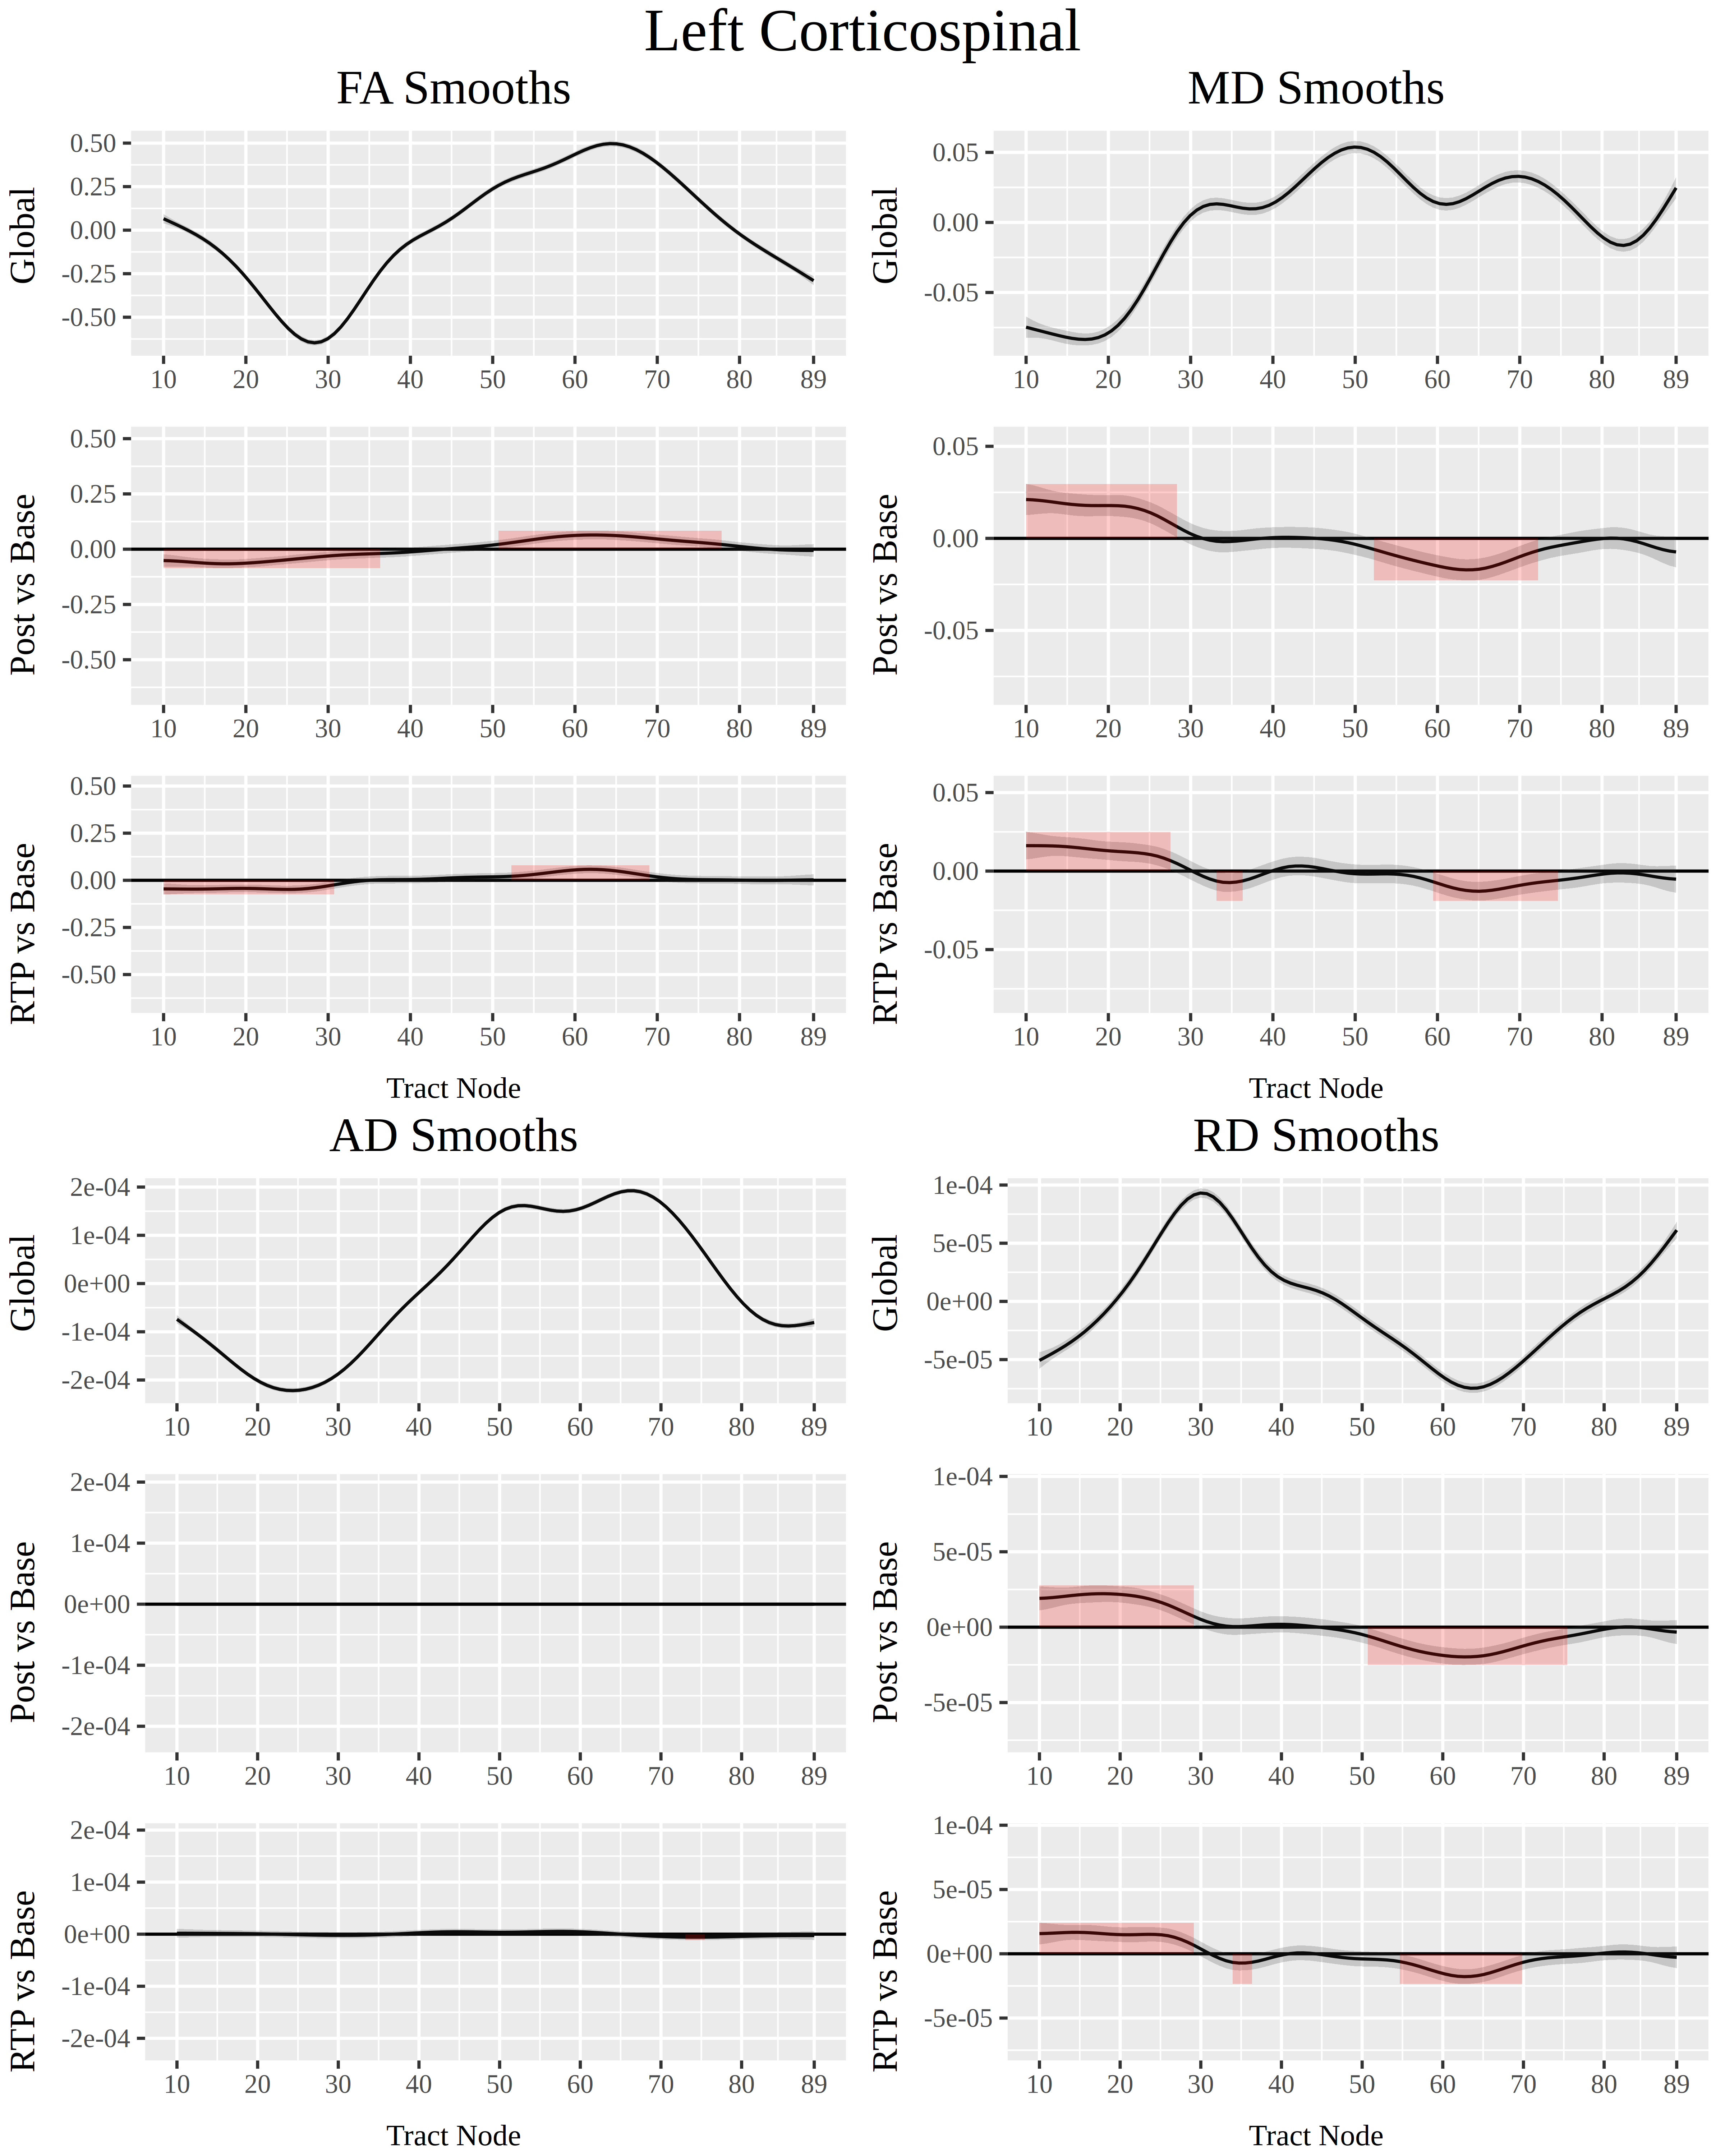
\includegraphics[width=3in]{fit_LGIO_lCS.png}}
	\subfloat[]{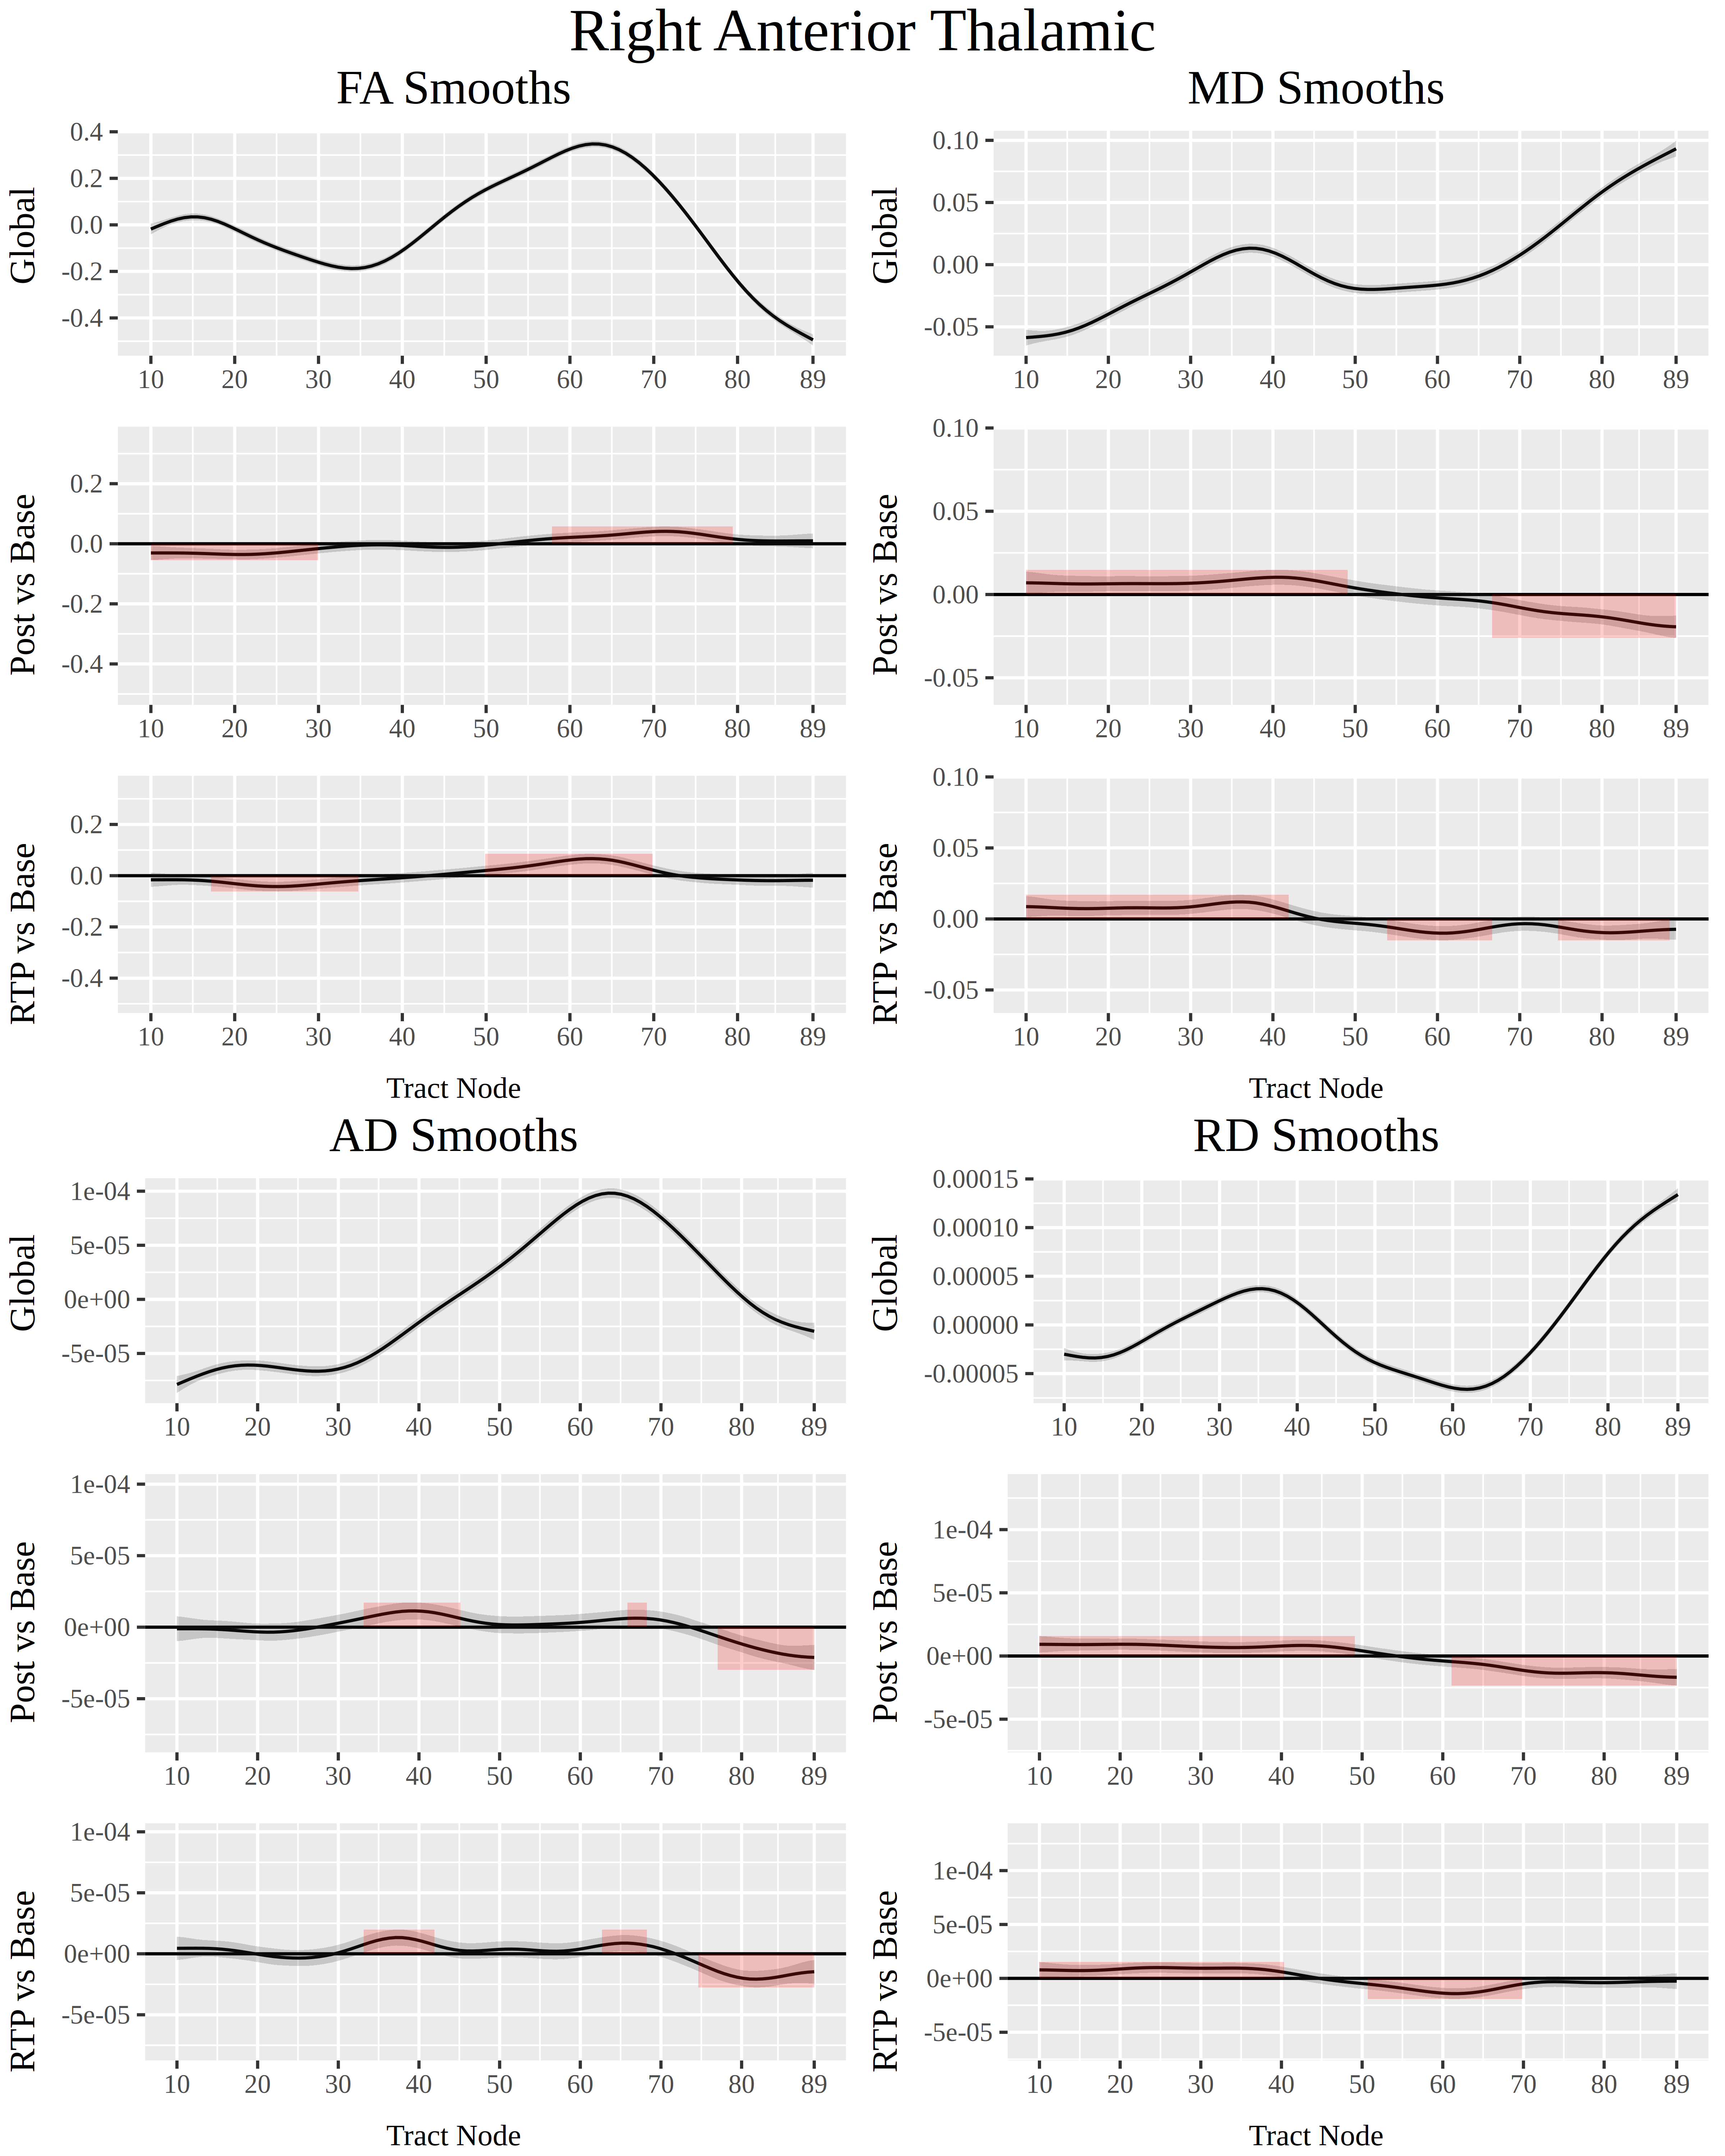
\includegraphics[width=3in]{fit_LGIO_raThal.png}}\\
	\subfloat[]{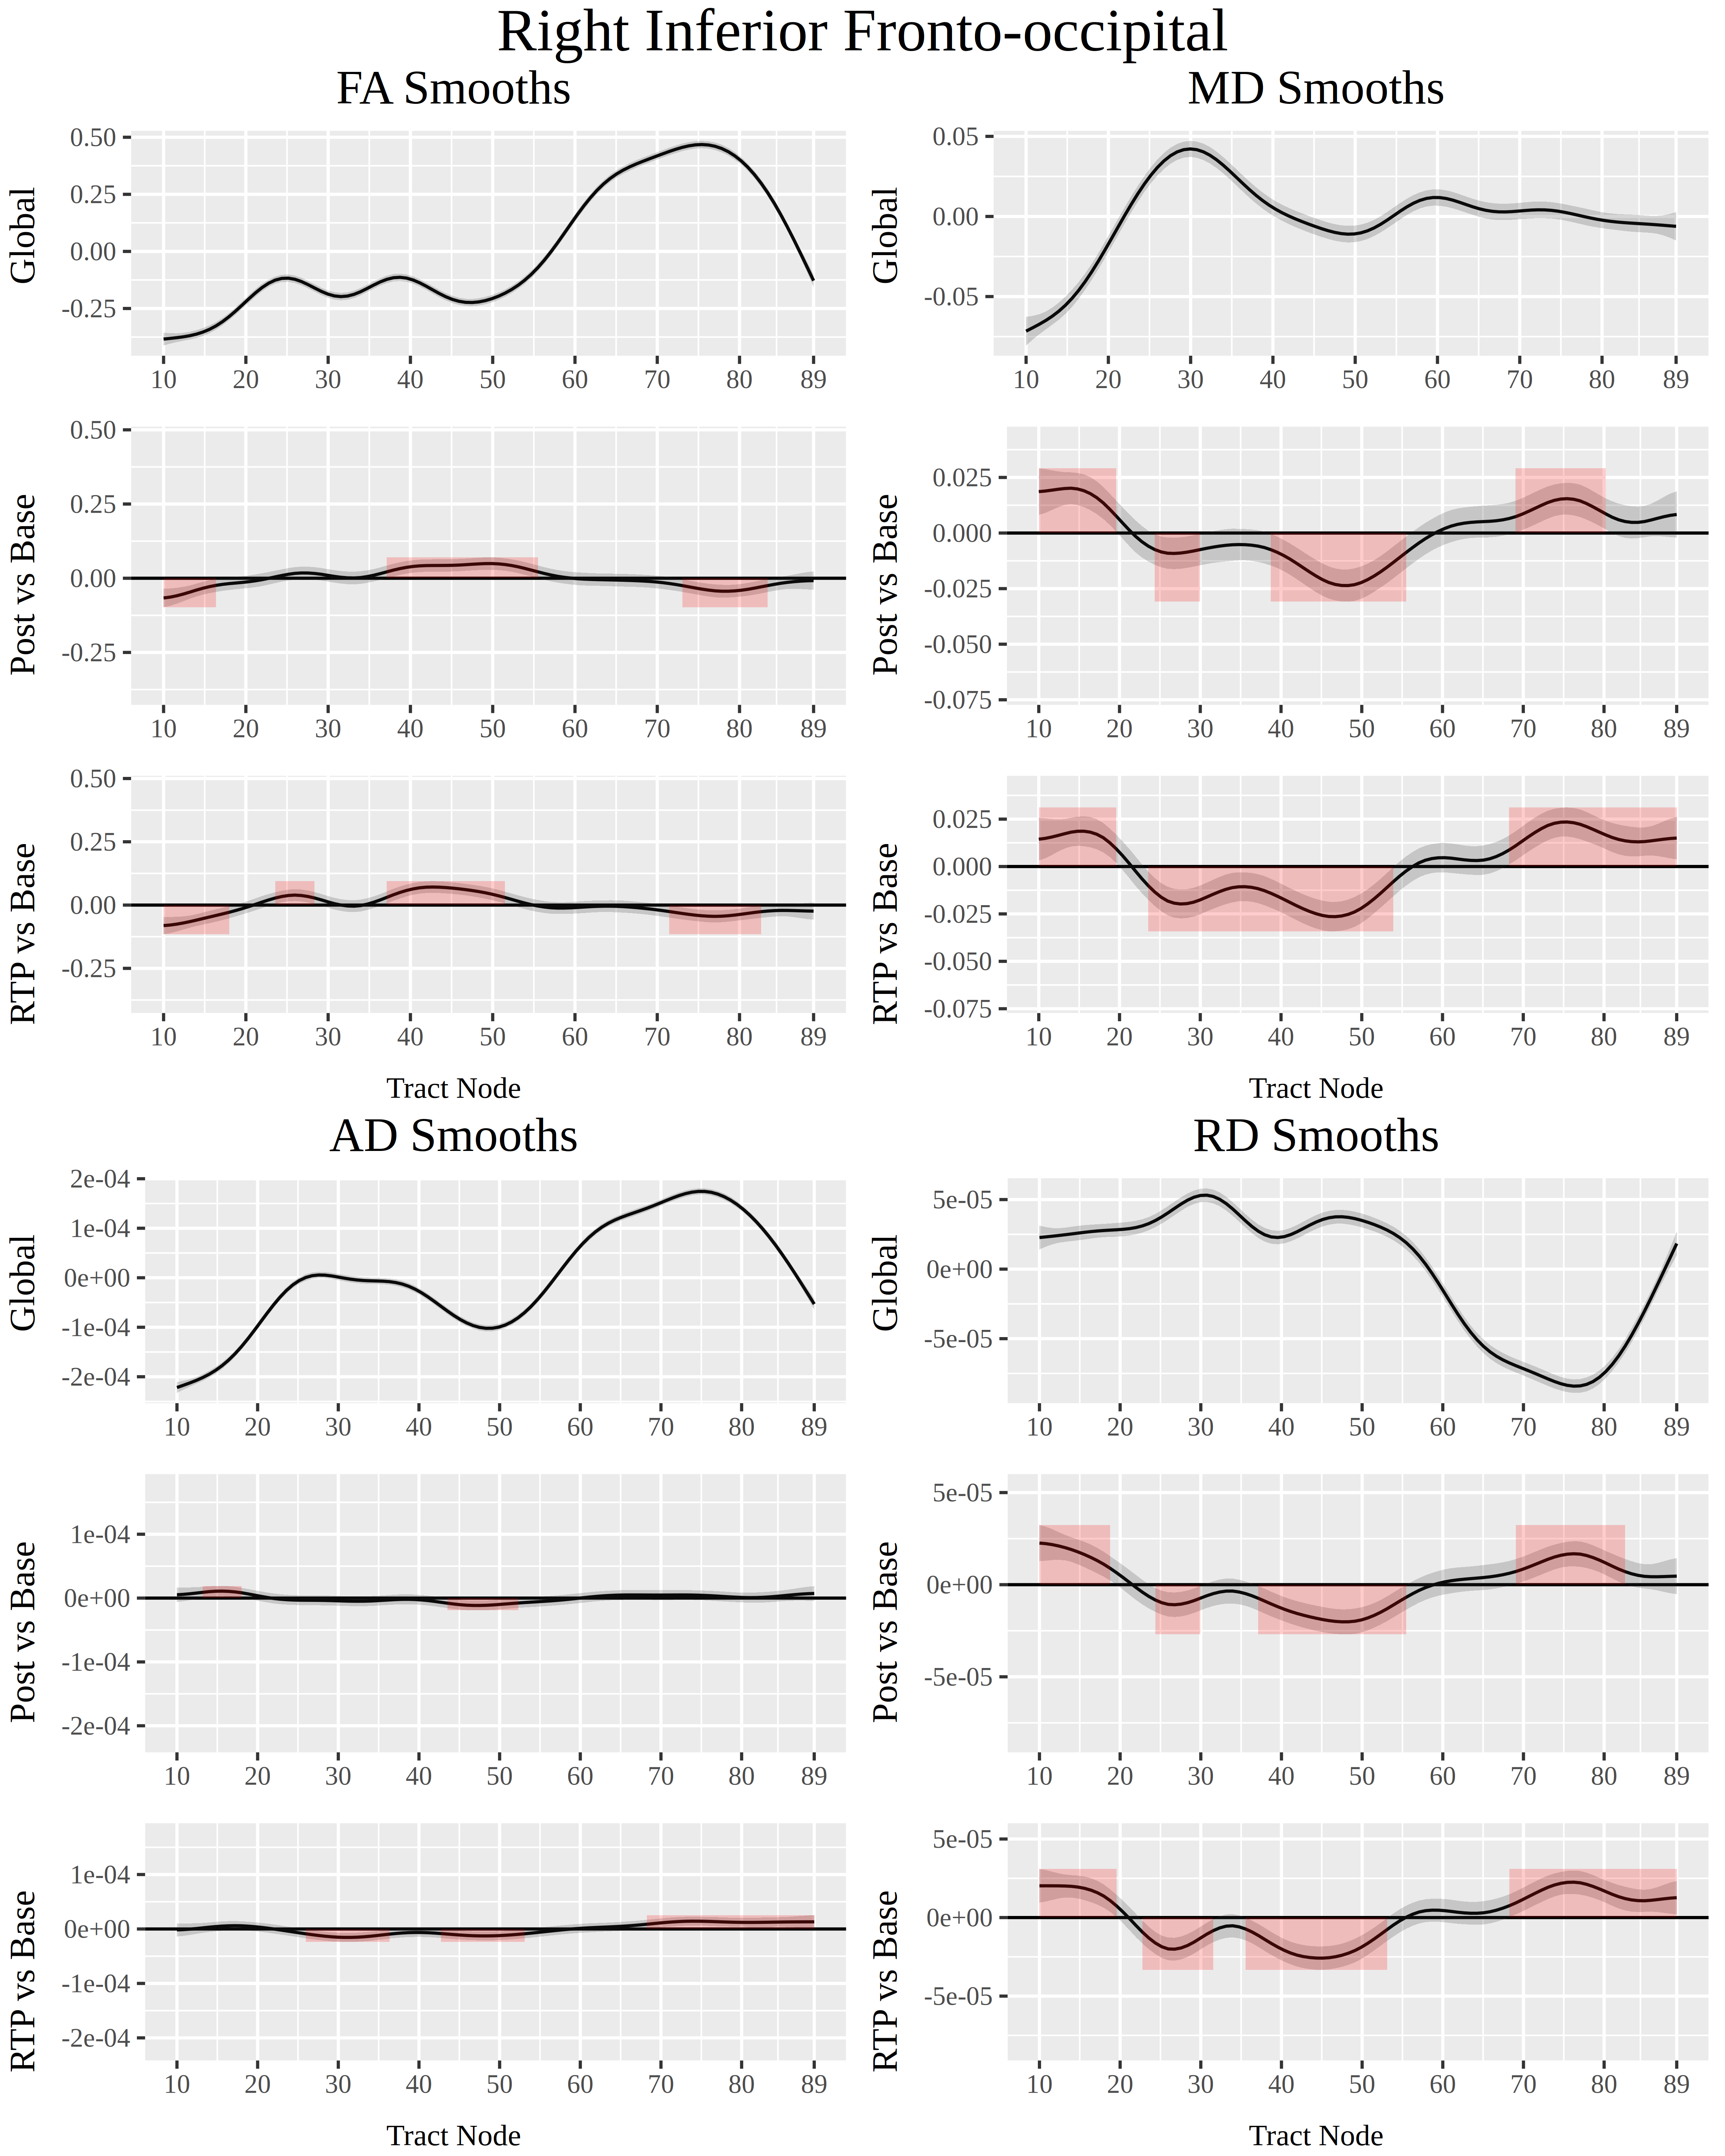
\includegraphics[width=3in]{fit_LGIO_rIFO.png}}
	\captionsetup{margin={0mm,0cm}}
	\caption{(a) Left corticospinal smooths indicate Post vs. Base increased FA at node 60, driven by RD decrease, which remains unchanged by RTP. (b) Right anterior thalamic and (c) right inferior fronto-occipital smooths reveal the same pattern about nodes 65 and 45, respectively.}
	\label{supp-fig:lgio-gam-norecov}
\end{figure}

\end{document}